\chapter{Resultado Numéricos}\label{resul_numericos}


\section*{Aplicação em imagem simulada}
A metodologia (MLE) para a detecção será aplicada para uma imagem simulada baseada em~\cite{nhfc,gamf}. A imagem tem $400\times400$ pixels e foi gerada por duas amostras obedecendo a distribuíção Wishart. Para cada par de matrizes de covariância $\Sigma_{k_1}$, $\Sigma_{k_2}$ a imagem $I_{k_1,k_2}$ é simulada de acordo com, amostras de $W_G(\Sigma_{k_1}, 4)$ para a metade esquerda da imagem, e  amostras $W_G(\Sigma_{k_2}, 4)$ para a metade direita da imagem.


A imagem $400 \times 400$ pixels foi gerada
\begin{figure}[hbt]
	\centering
	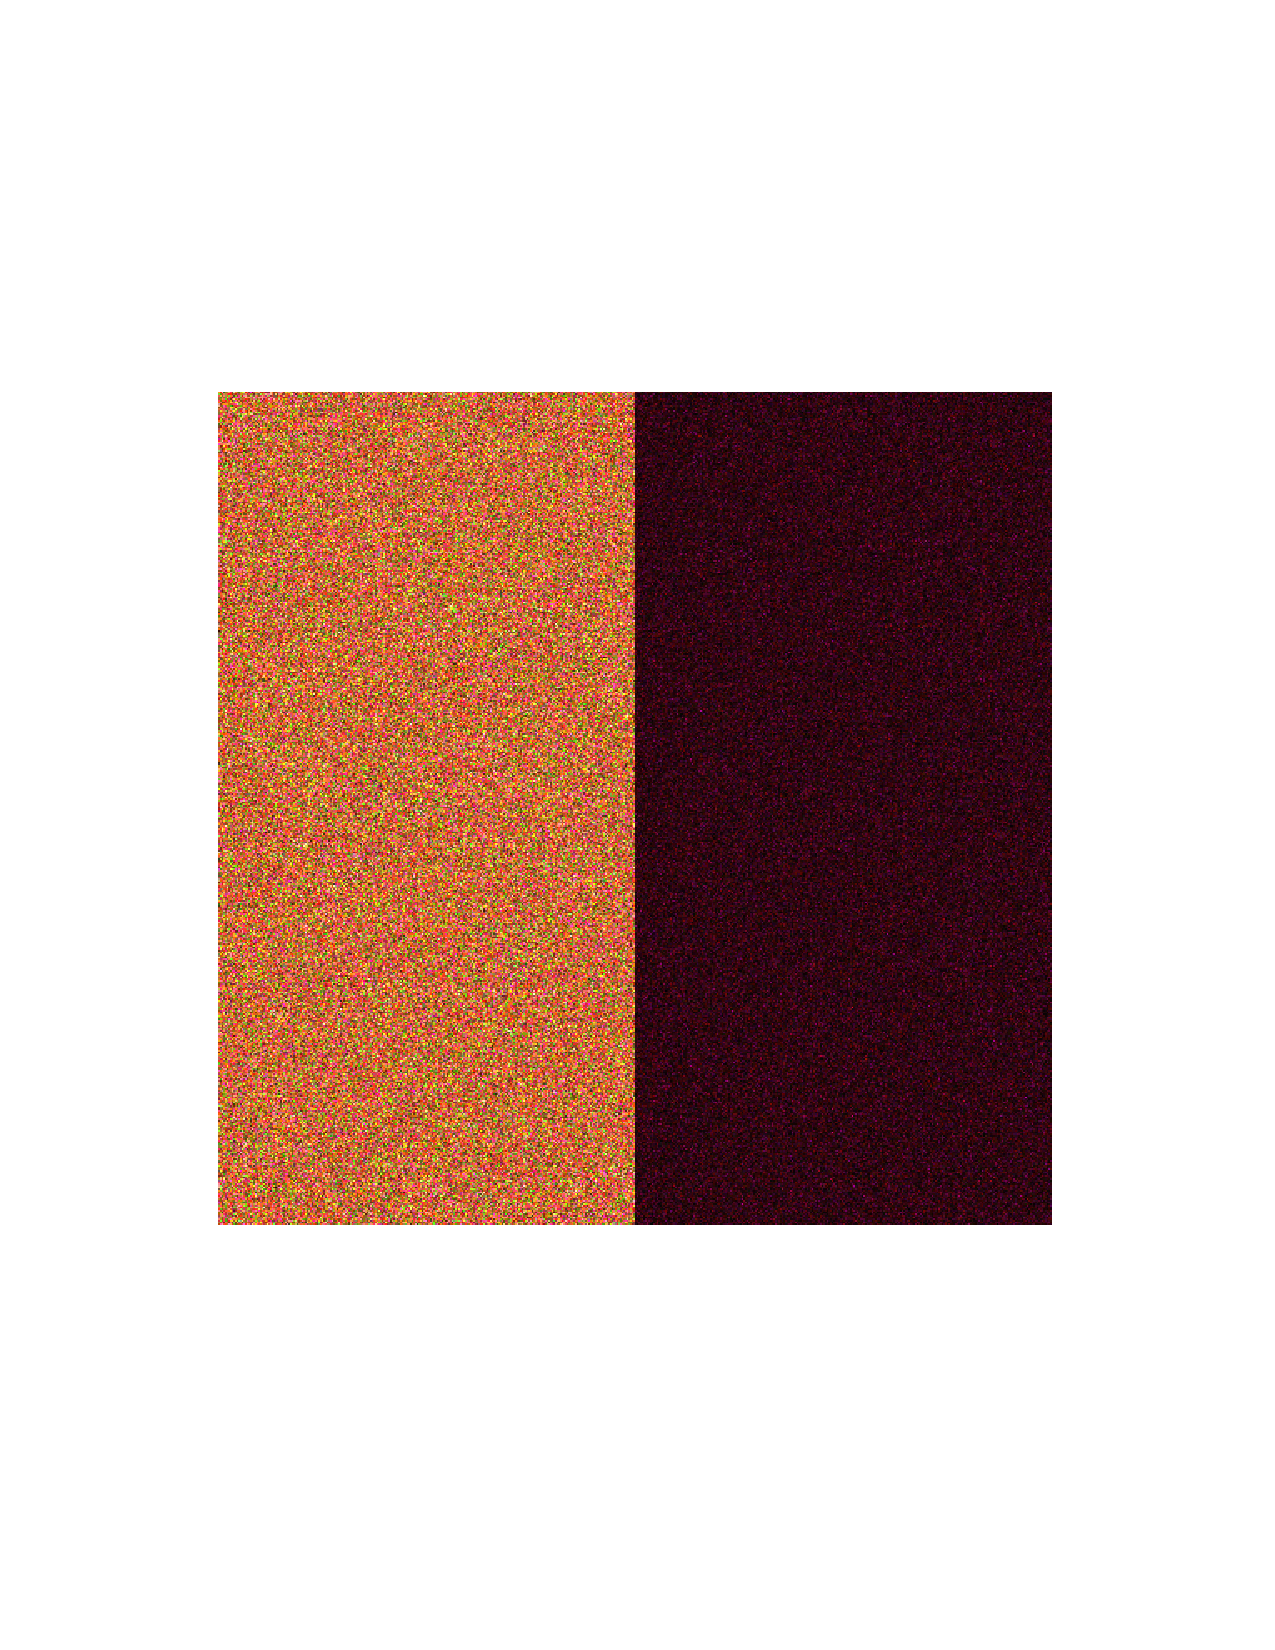
\includegraphics[width=.7\linewidth]{phanton_gamf_dec_pauli}%
	\caption{Decomposição de Pauli}
\label{fig:simulada_gamf_dec_pauli}
\end{figure}

A decomposição de Pauli é baseada na combinação linear dos canais de intensidades, 
$$(\mathbf{I_\text{hh}+I_{\text{vv}}}, \mathbf{I_\text{hh}-I_{\text{vv}}}, \mathbf{I_\text{hv}}).$$ 
Esta decomposição mostra a evidência de bordas em uma linha média da imagem, como apresentado na figura~\ref{fig:simulada_gamf_dec_pauli}. 
\subsubsection*{Distribuição univariada $\Gamma$ com L fixo}

A imagem simulada  usa as intensidades da matriz de covariancia $\Sigma_{k_1}$ e $\Sigma_{k_2}$ definidas por
\begin{equation}\label{matriz_sigma_gamf_1}
	\hspace{2.75cm} \Sigma_{u}= \left[
\begin{array}{lll}
0.042811            & 0.000072-0.003180i & 0.010435+0.005022i\\
0.000072+0.003180i  & 0.035977           & 0.000784+0.004886i\\
0.010435-0.005022i  & 0.000784-0.004886i & 0.066498
\end{array}
\right],
\end{equation}
\begin{equation}\label{matriz_sigma_gamf_2}
 \Sigma_{f}= \left[
\begin{array}{lll}
0.014380            & 0.001333-0.000076i & -0.000755+0.001570i\\
0.001333+0.000076i  & 0.002789           & -0.001044+0.001101i\\
-0.000755-0.001570i &-0.001044-0.001101i & 0.015387
\end{array}
\right],
\end{equation}
as intensidades são as entradas da diagonal principal.  
    
\begin{figure}[hbt]
	\centering
     \subfloat[Canal $\text{hh}$ \label{fig:evid_bordas_l:1a}]{%
       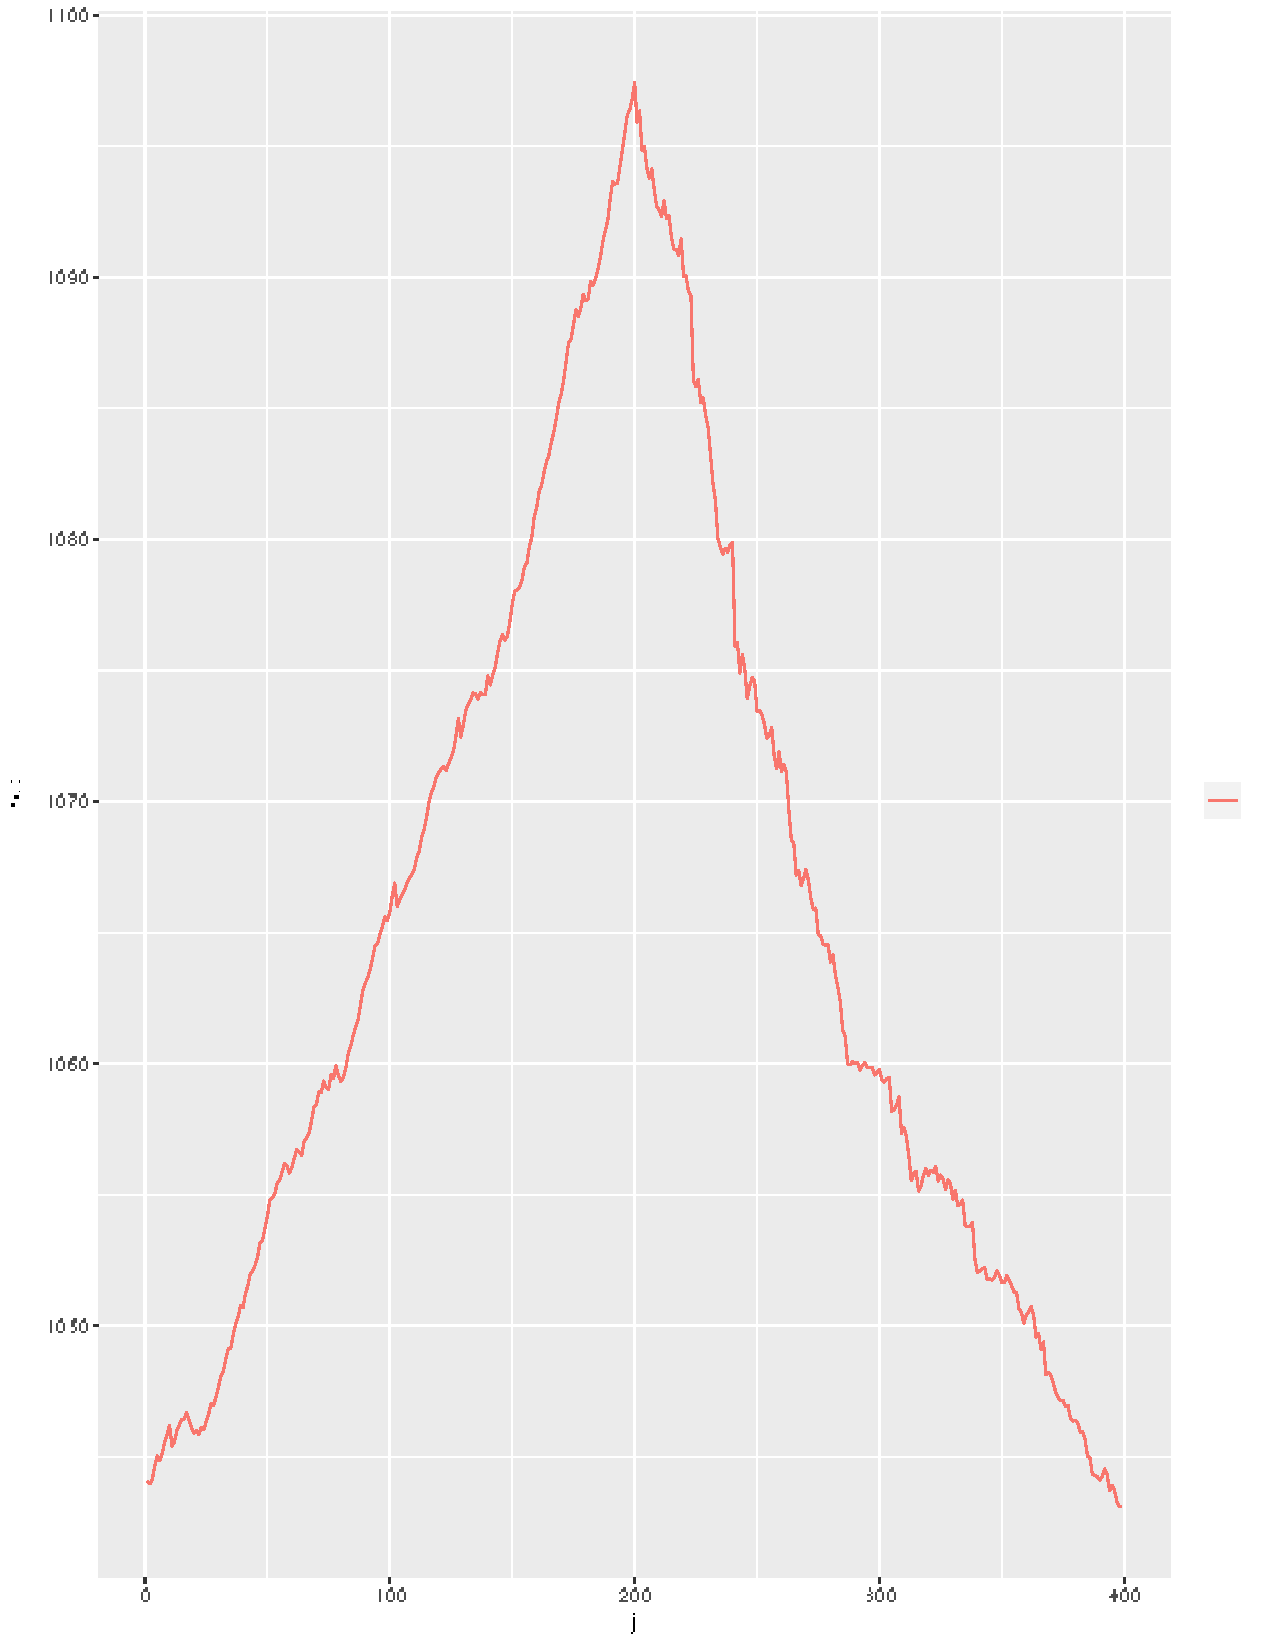
\includegraphics[width=0.32\linewidth]{grafico_l_gamf_2017_sigmahh_param_mu}}
     \subfloat[Canal $\text{hv}$ \label{fig:evid_bordas_l:1b}]{%
       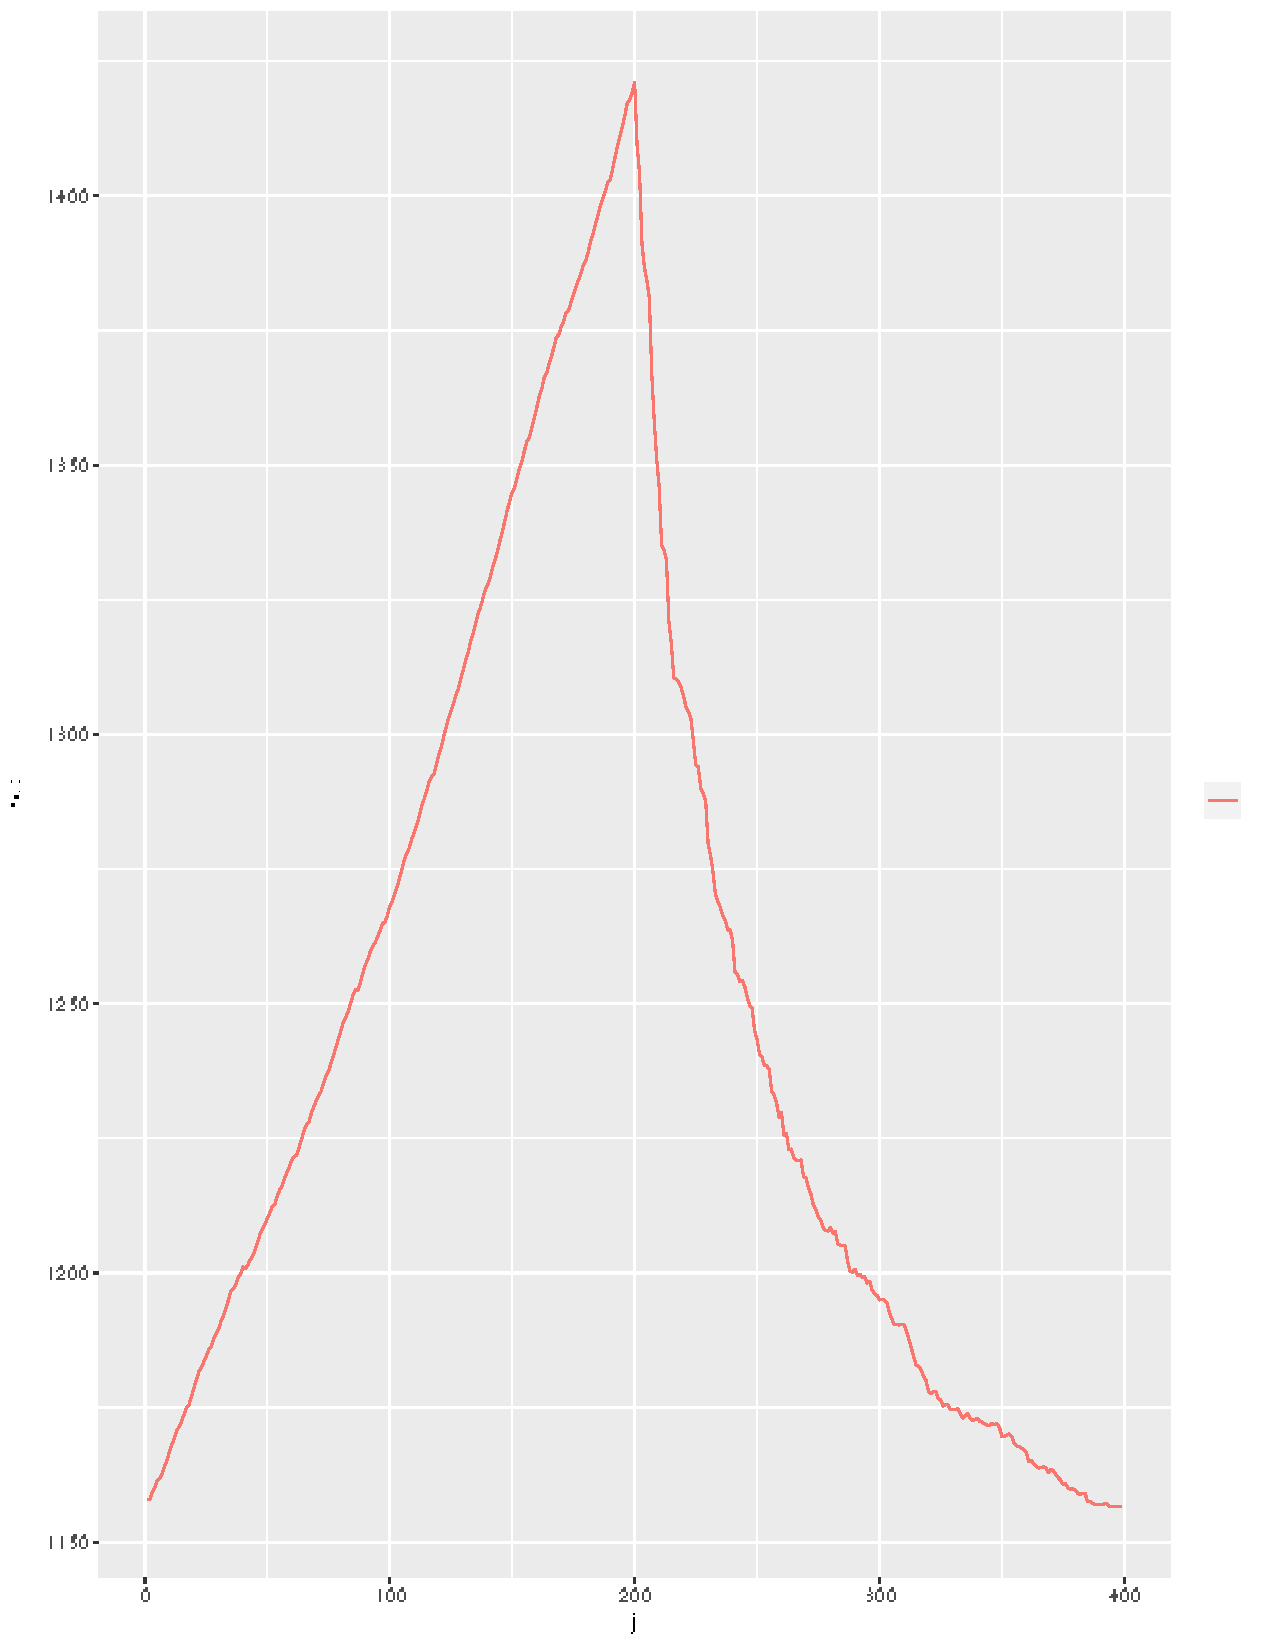
\includegraphics[width=0.32\linewidth]{grafico_l_gamf_2017_sigmahv_param_mu}}
     \subfloat[Canal $\text{vv}$ \label{fig:evid_bordas_l:1c}]{%
       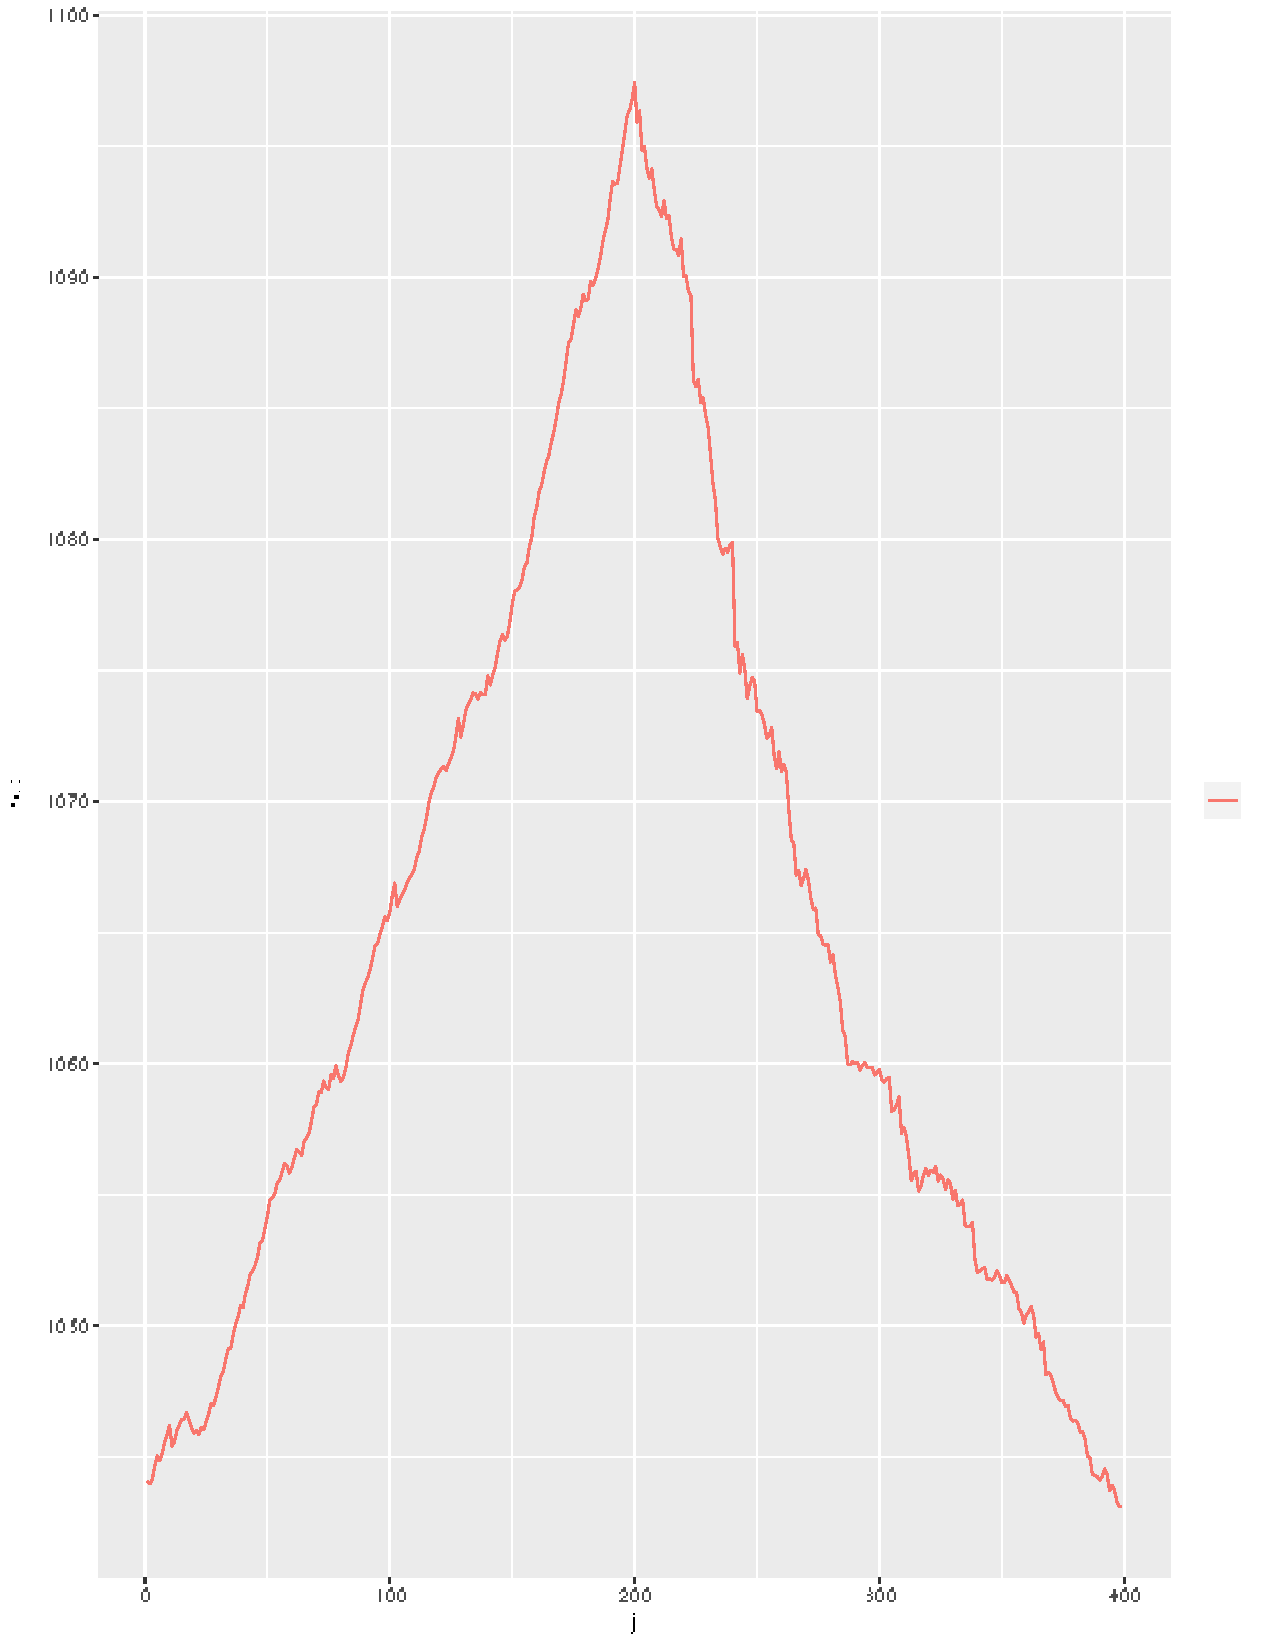
\includegraphics[width=0.32\linewidth]{grafico_l_gamf_2017_sigmahh_param_mu}}
     \caption{Funções log-verossimilhanças para a radial 150}
     \label{fig:evid_bordas_l}
   \end{figure}	

As funções da figura \eqref{fig:evid_bordas_l} mostram picos indicando evidência de bordas a ser encontrada, porém as funções não são suaves dificultando o uso de métodos de otimização que calculam a derivada da função. O problema foi resolvido usando o método \textit{Simulated Annealing} generalizado (GenSA)~~\cite{xgsh}, adequado para funções não diferenciáveis.


O método da máxima verossimilhança \eqref{eq:TotalLogLikelihood} foi aplicado na imagem simulada com duas amostras, e as evidências de bordas estão mostradas na figura \eqref{evidencias_hh_hv_vv_gamf}.

 \begin{figure*}[hbt]
	\centering
     \subfloat[Evidências no canal $\text{hh}$  \label{evidencias_hh_hv_vv_gamf_mu_estimado:a}]{%
       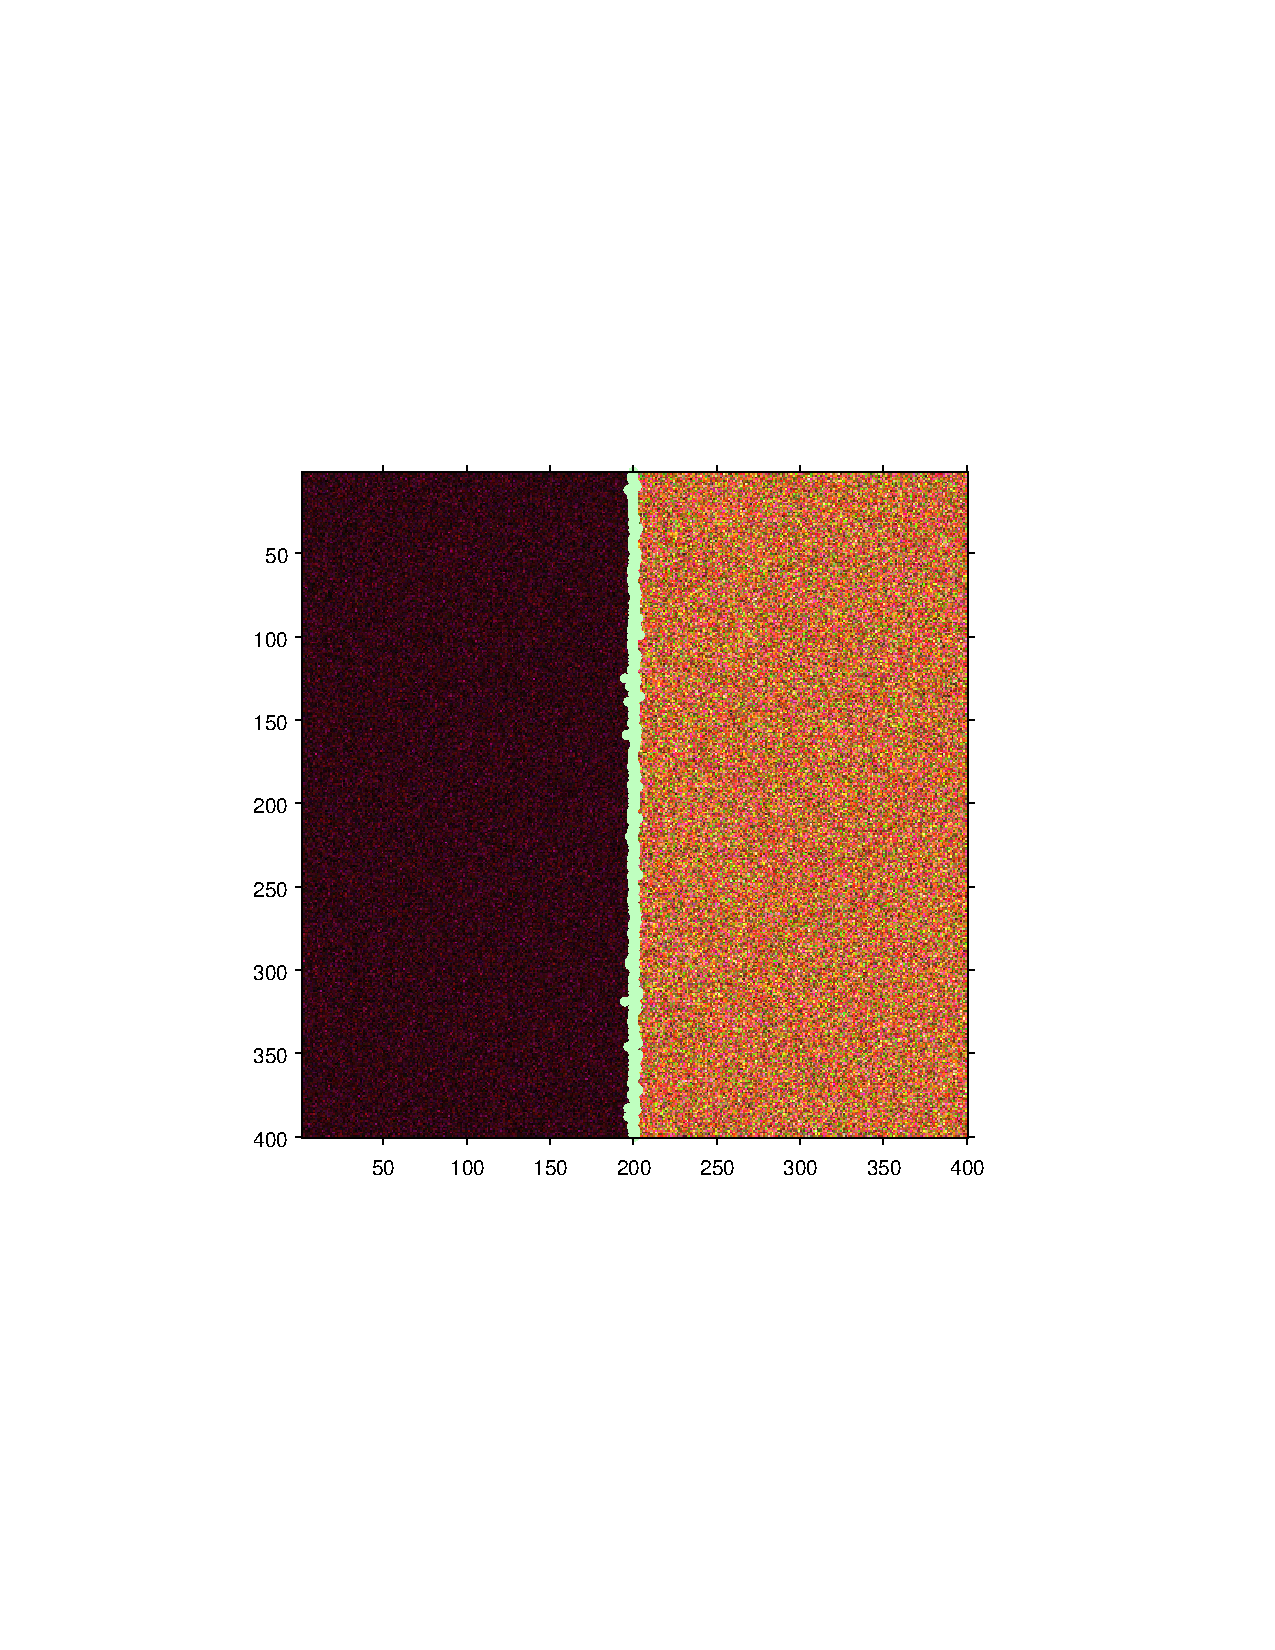
\includegraphics[width=0.35\linewidth]{im_sim_gamf_hh_evid_param_mu_14_pixel}
     }
     \subfloat[Evidências no canal $\text{hv}$ \label{evidencias_hh_hv_vv_gamf_mu_estimado:b}]{%
       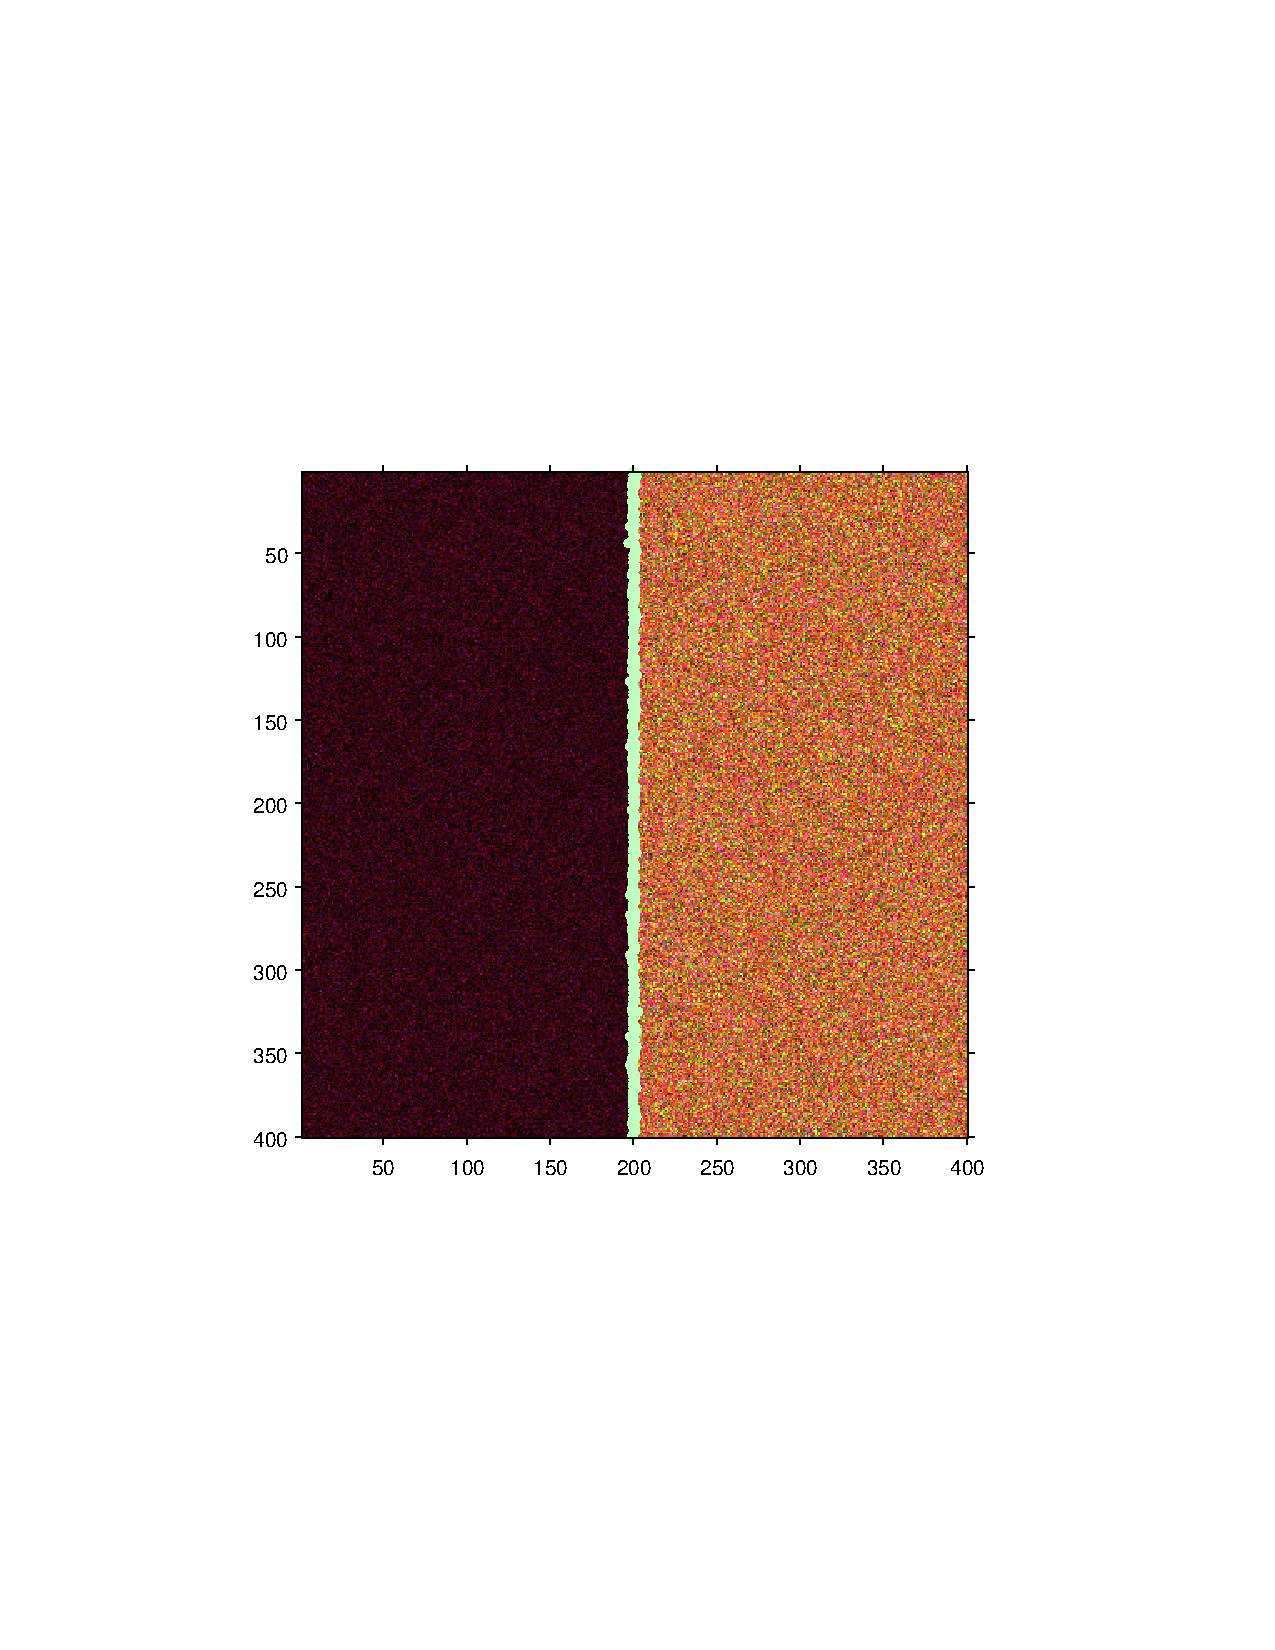
\includegraphics[width=0.35\linewidth]{im_sim_gamf_hv_evid_param_mu_14_pixel}
     }      
     \subfloat[Evidências no canal $\text{vv}$ \label{evidencias_hh_hv_vv_gamf_mu_estimado:c}]{%
       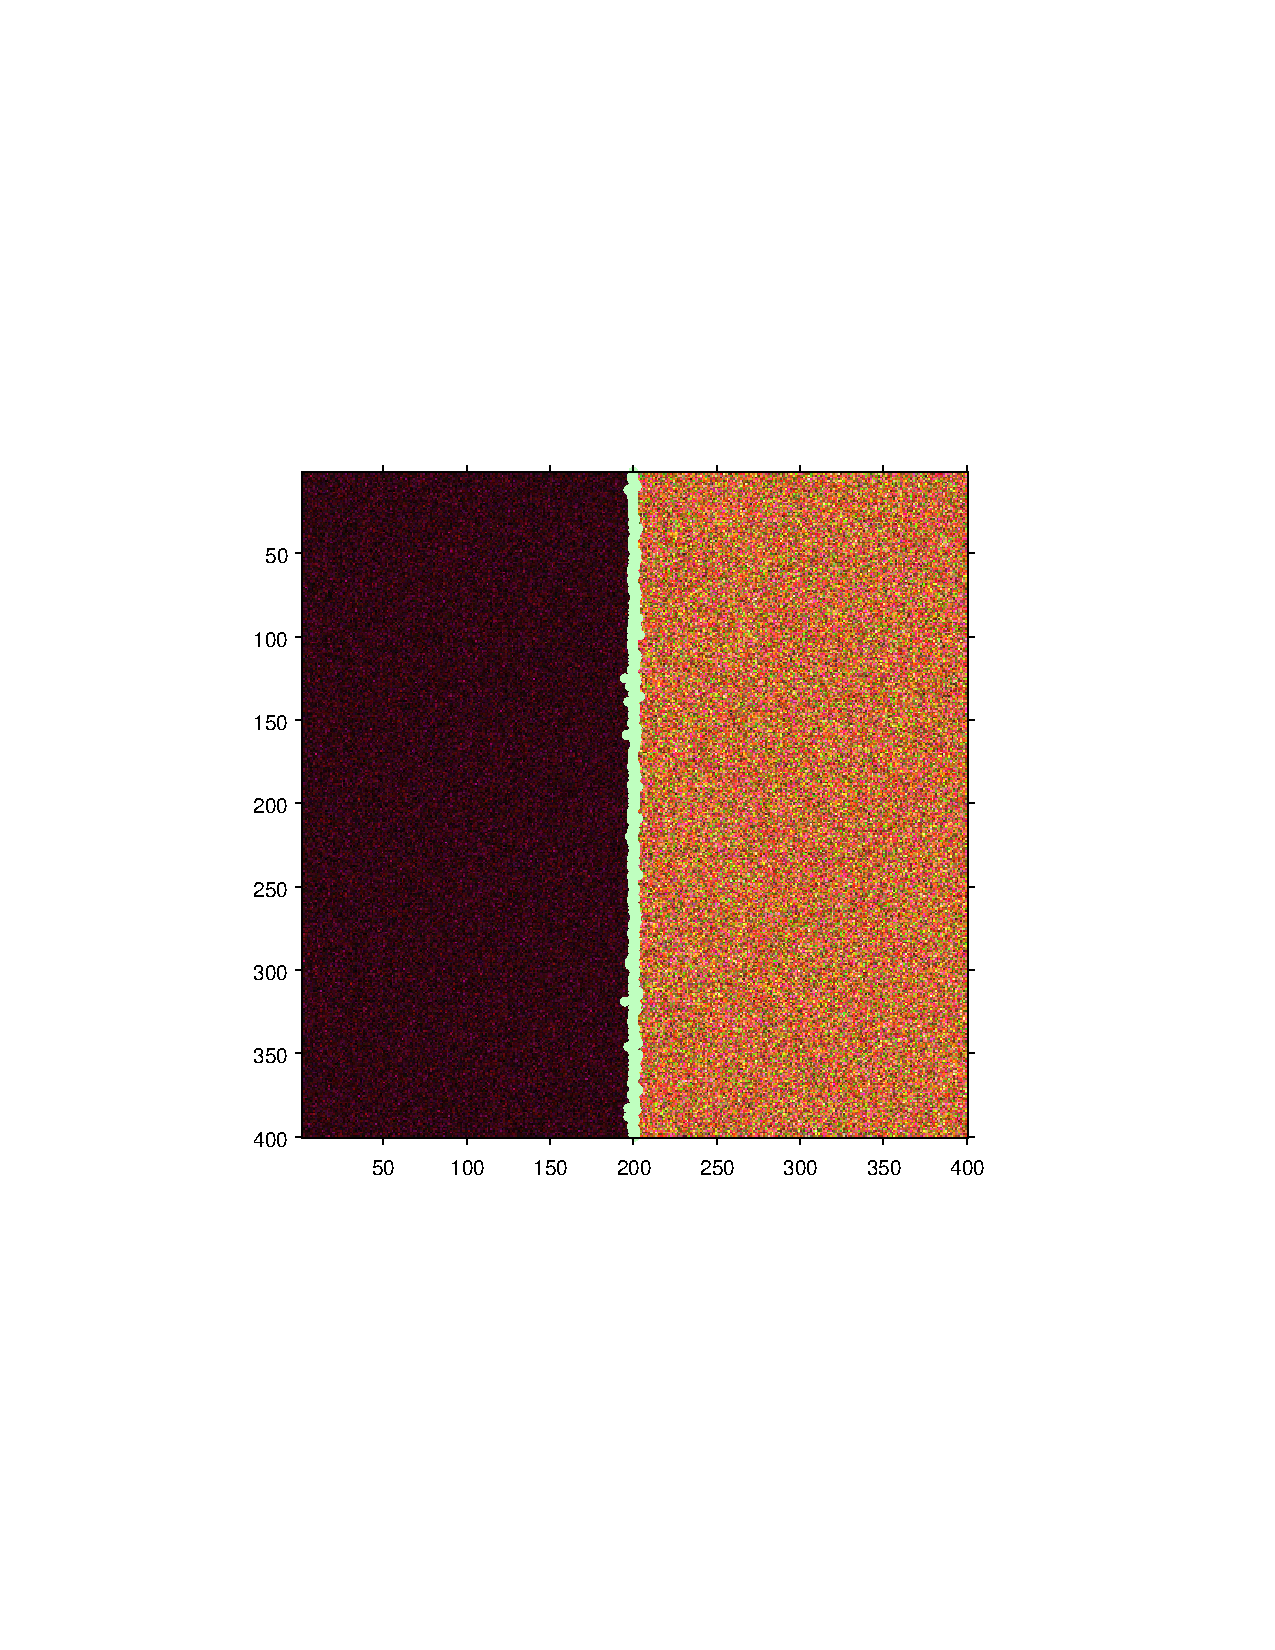
\includegraphics[width=0.35\linewidth]{im_sim_gamf_vv_evid_param_mu_14_pixel}
     }
    \caption{Evidências de bordas para os três canais de intensidade com $\mu$ estimado.}
     \label{evidencias_hh_hv_vv_gamf} 
   \end{figure*}
   
   
   
   
\begin{figure*}[hbt]
	\centering
     \subfloat[Evidências no canal $\text{hh}$  \label{evidencias_hh_hv_vv_gamf_mu_estimado:a}]{%
       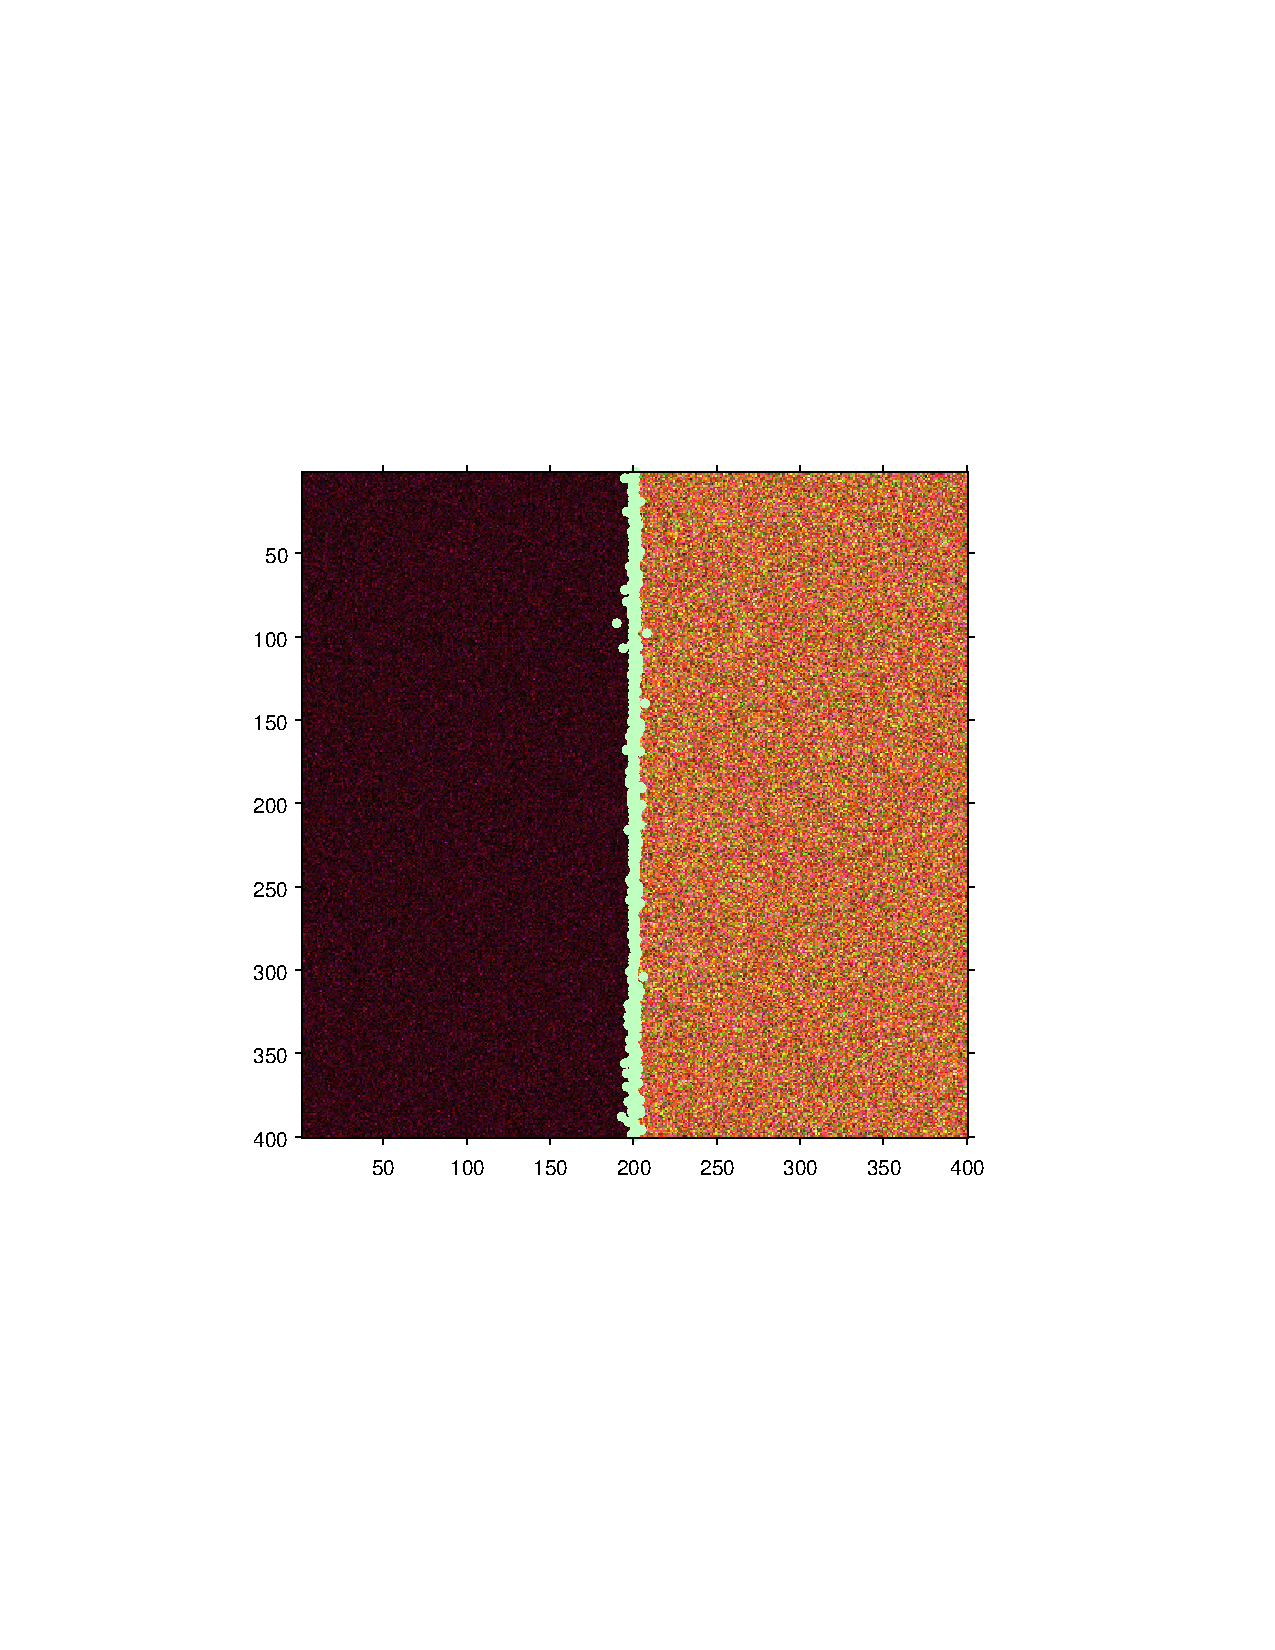
\includegraphics[width=0.35\linewidth]{im_sim_gamf_hh_evid_media_mu_14_pixel}
     }
     \subfloat[Evidências no canal $\text{hv}$ \label{evidencias_hh_hv_vv_gamf_mu_estimado:b}]{%
       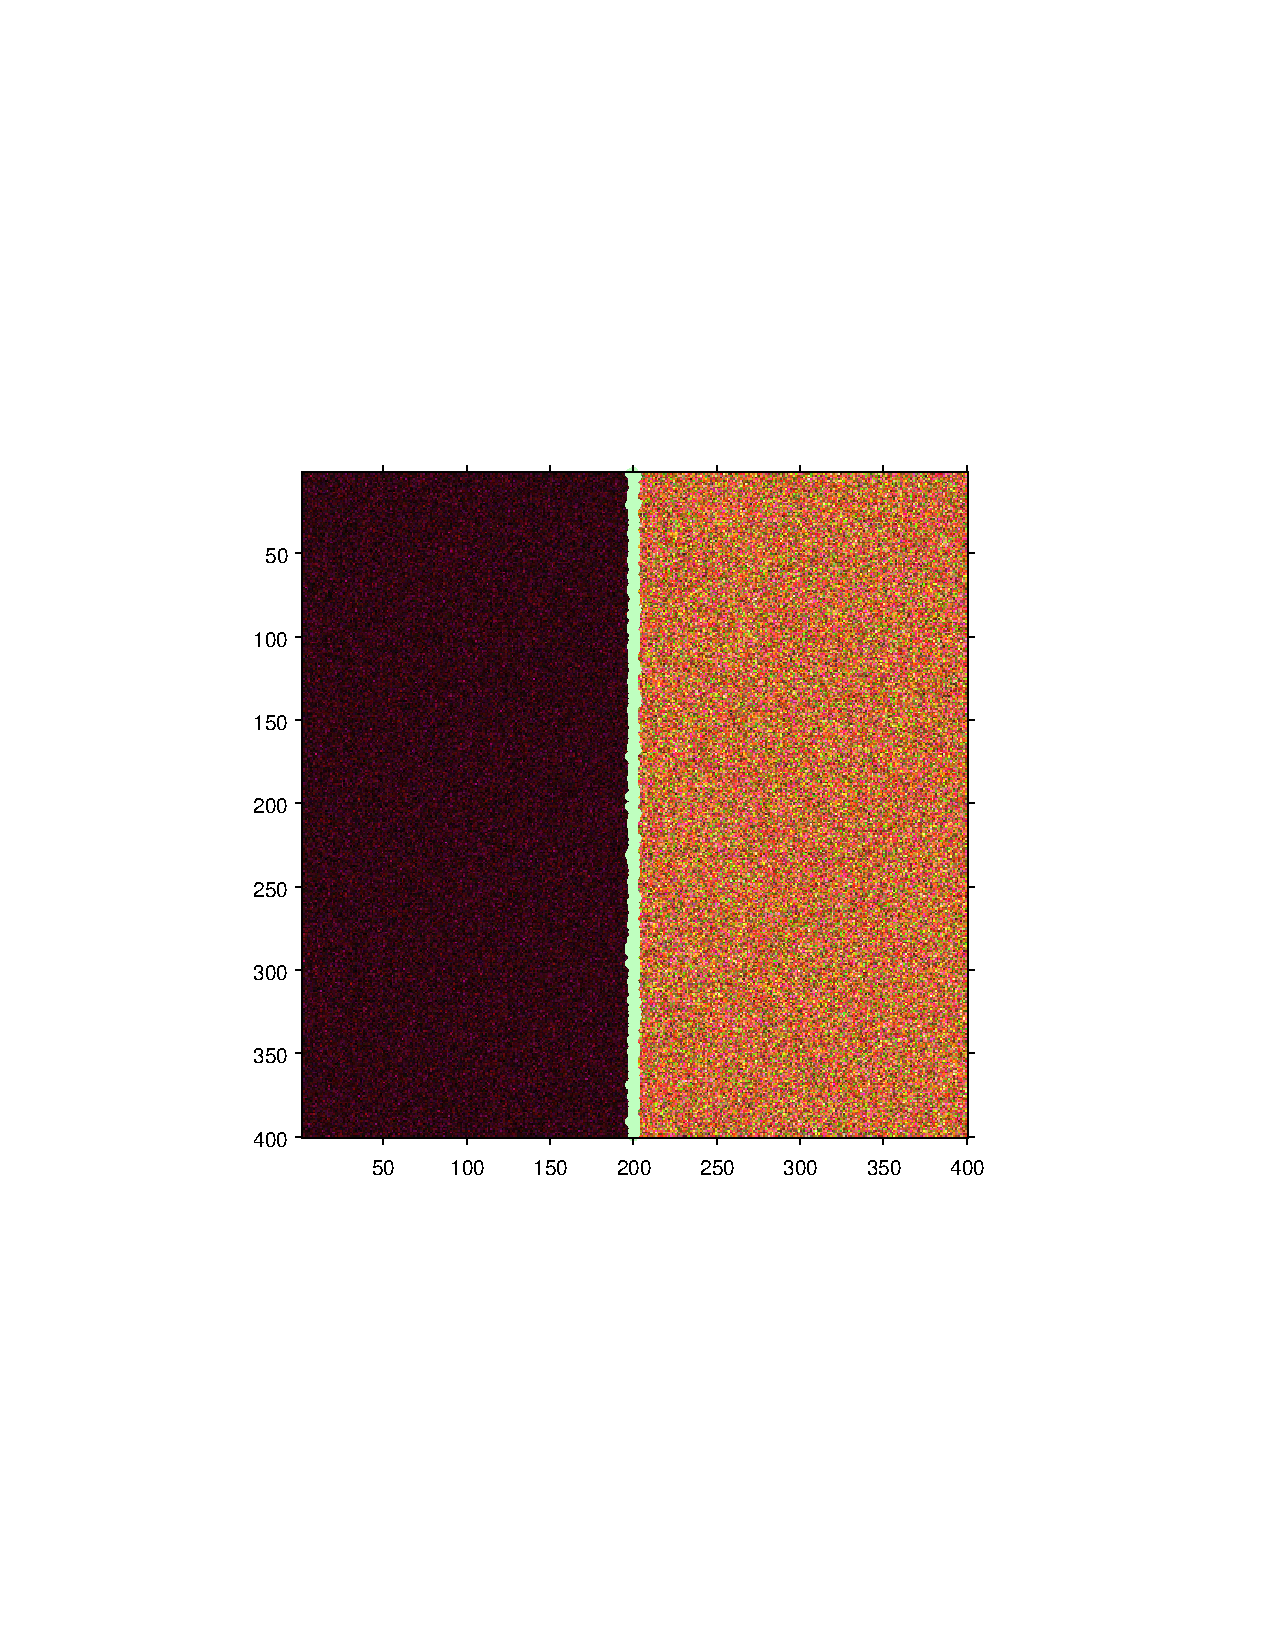
\includegraphics[width=0.35\linewidth]{im_sim_gamf_hv_evid_media_mu_14_pixel}
     }      
     \subfloat[Evidências no canal $\text{vv}$ \label{evidencias_hh_hv_vv_gamf_mu_estimado:c}]{%
       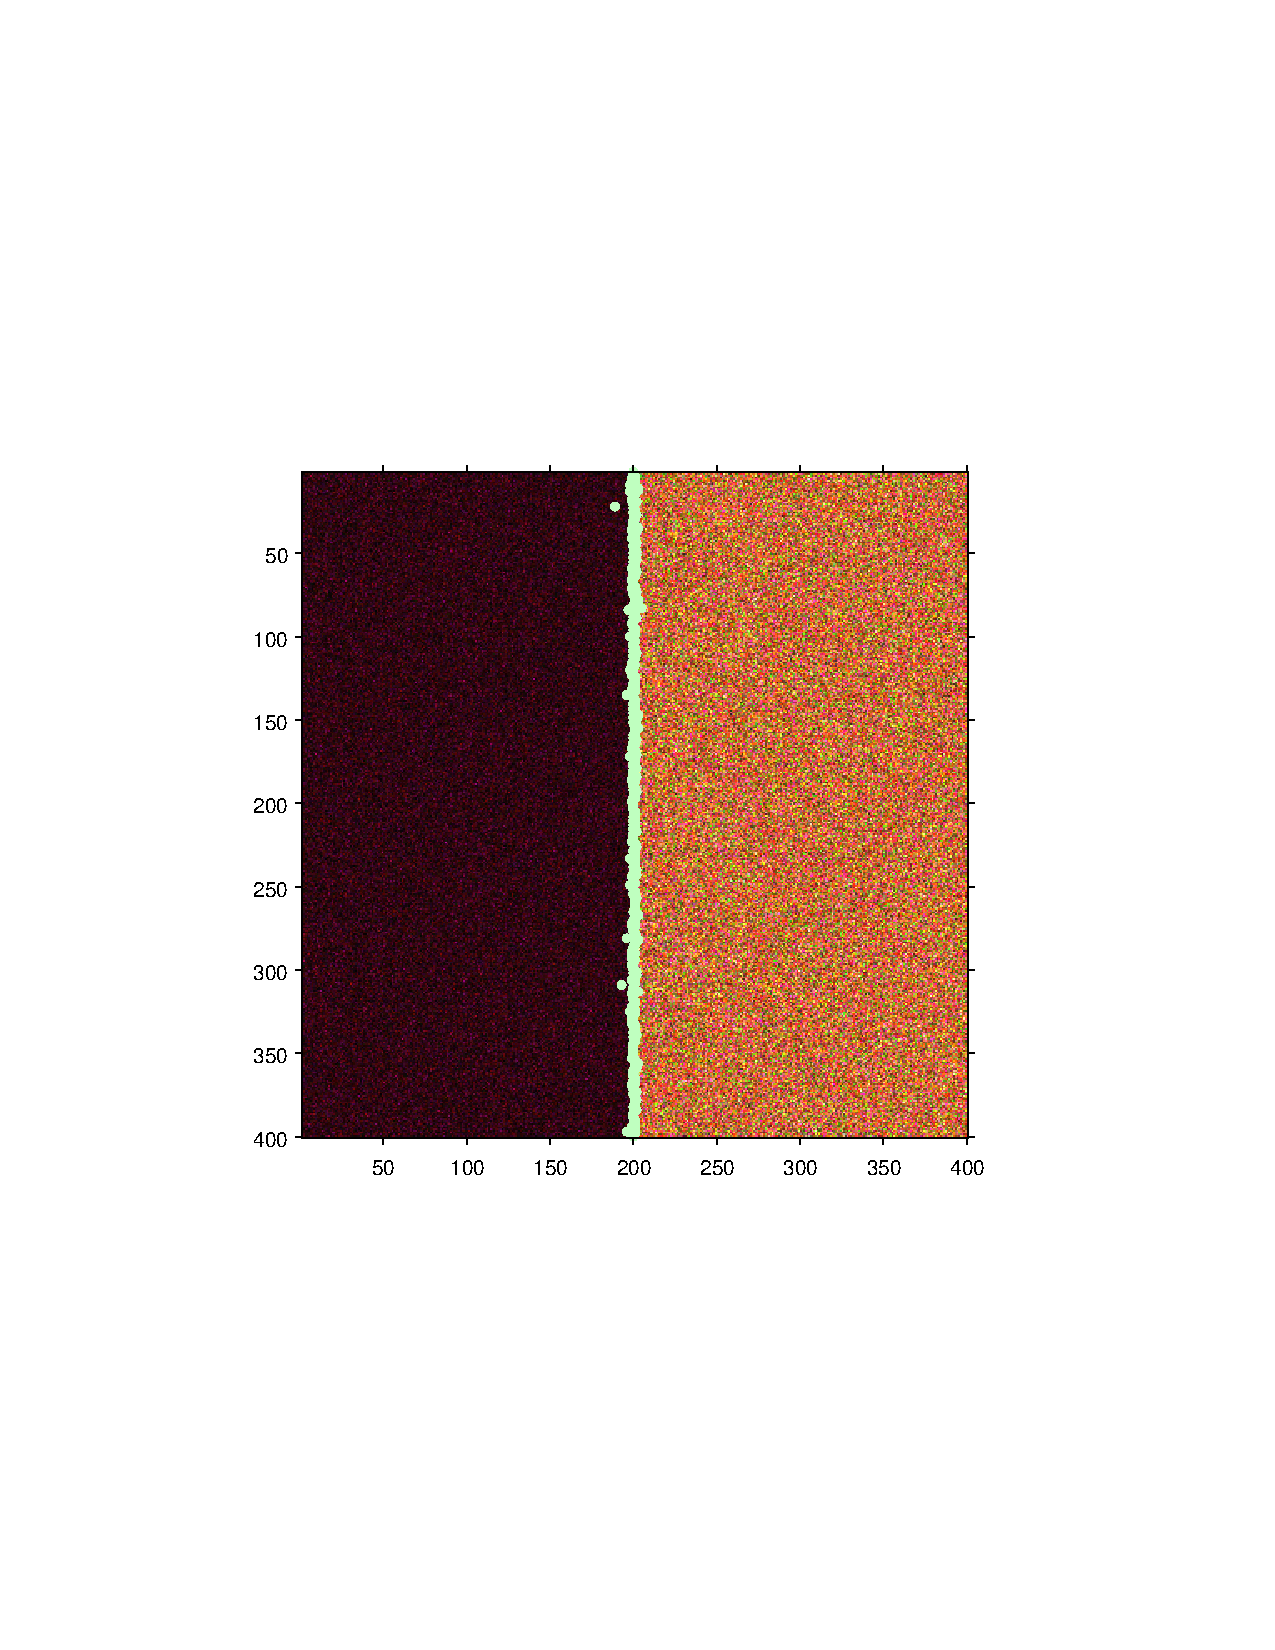
\includegraphics[width=0.35\linewidth]{im_sim_gamf_vv_evid_media_mu_14_pixel}
     }
    \caption{Evidências de bordas para os três canais de intensidade com $\mu$ estimado (media).}
     \label{evidencias_hh_hv_vv_gamf} 
   \end{figure*}



\subsubsection{Distribuição univariada produto de intensidades com L fixo}

A figura \eqref{fig:pdf_prod_mag_flat} mostra a distribuição univariada produto de magnitudes para radial(linha) 35 fixada e nessa radial escolhemos arbitrariamente o pixel igual a 150 para construir as funçoes de maxima verossimilhança. Notamos nas figuras o quanto a funçao é plana evidenciando a dificuldade para encontrar o $\rho$ máximo. A difuldade de encontrar o máximo teve consequência na construção da função de log-verossimilhança usando as estimativas de $\rho$, as funções apresentaram forte oscilação não sendo possível encontrar evidência de borda para a distribuição produto de intensidades. 

\begin{figure}[hbt]
	\centering
     \subfloat[Função $\ell$ para pixels de 1 até 150 \label{fig:pdf_prod_mag_flat:1a}]{%
       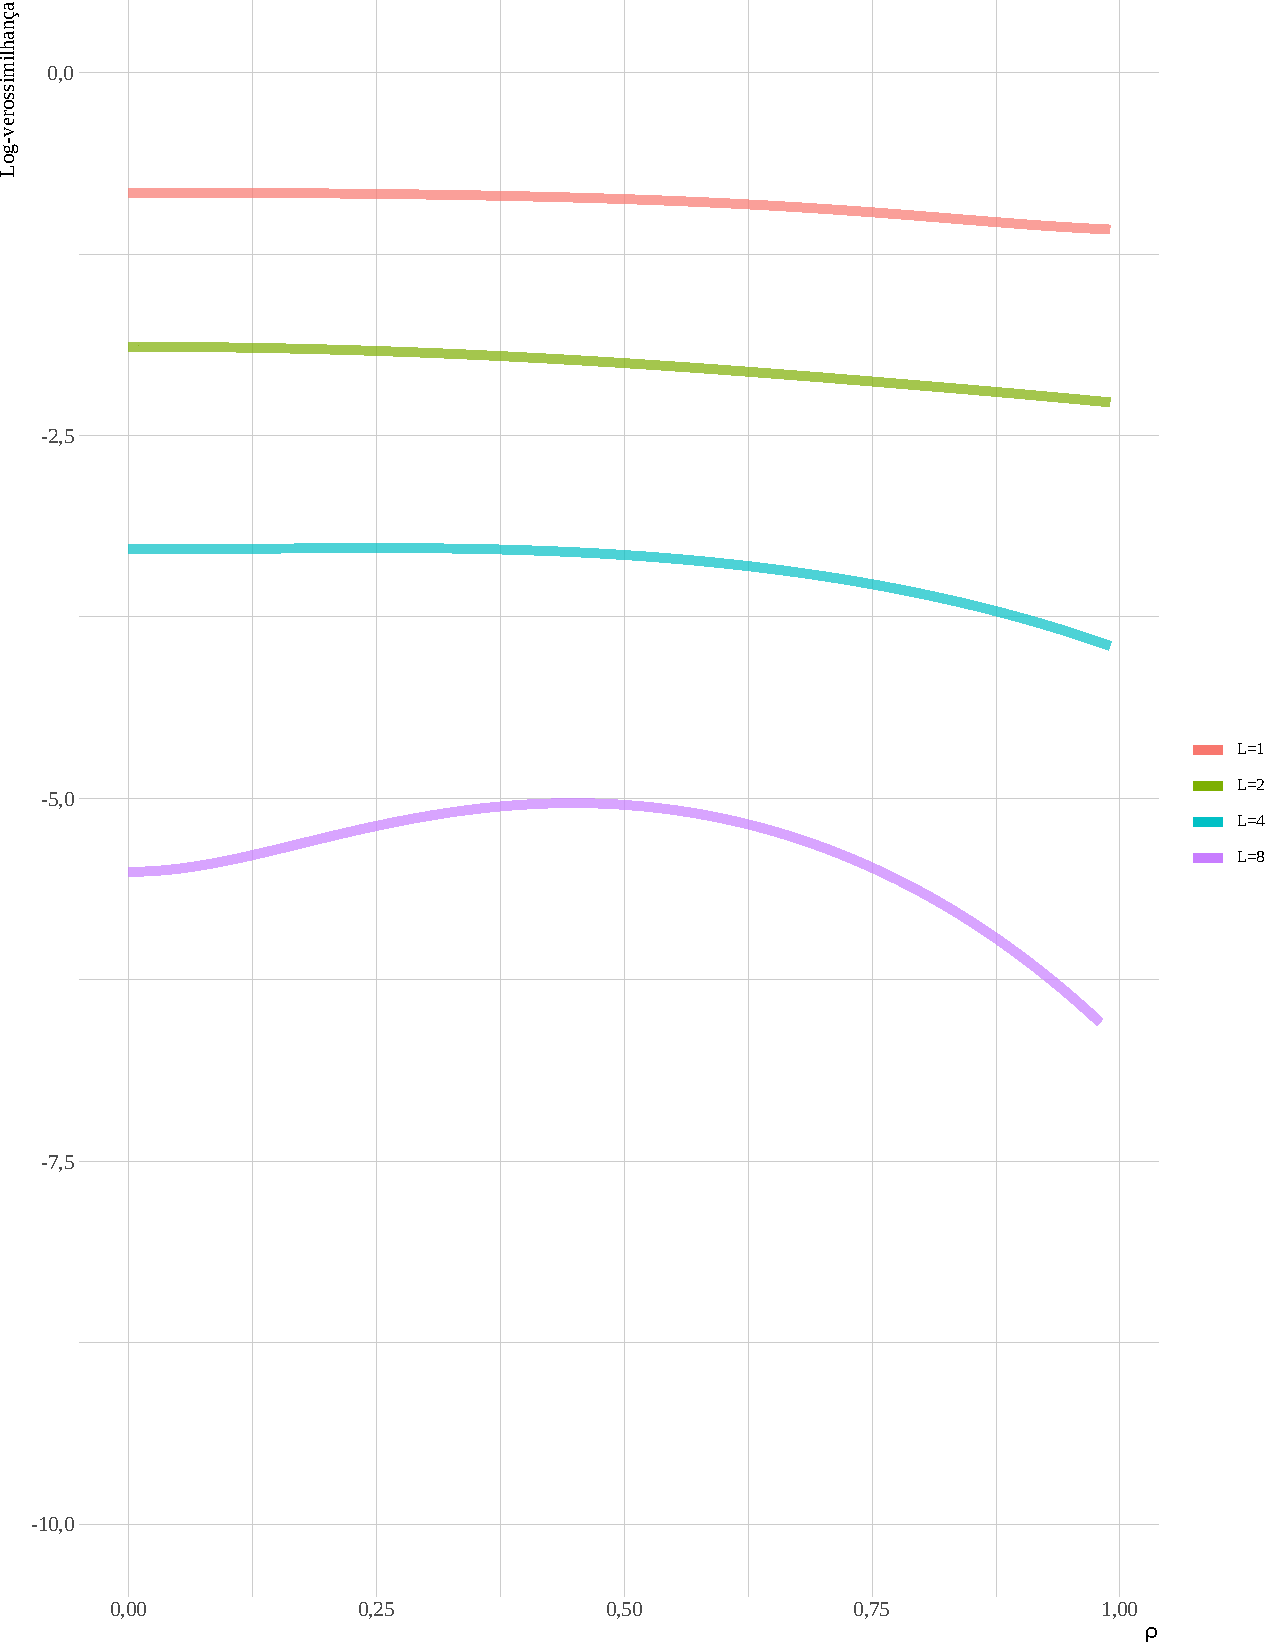
\includegraphics[width=0.32\linewidth]{log_like_prod_mag_L_fixo_por}}
     \subfloat[Função $\ell$ para pixels de 150 até 400 \label{fig:pdf_prod_mag_flat:1b}]{%
       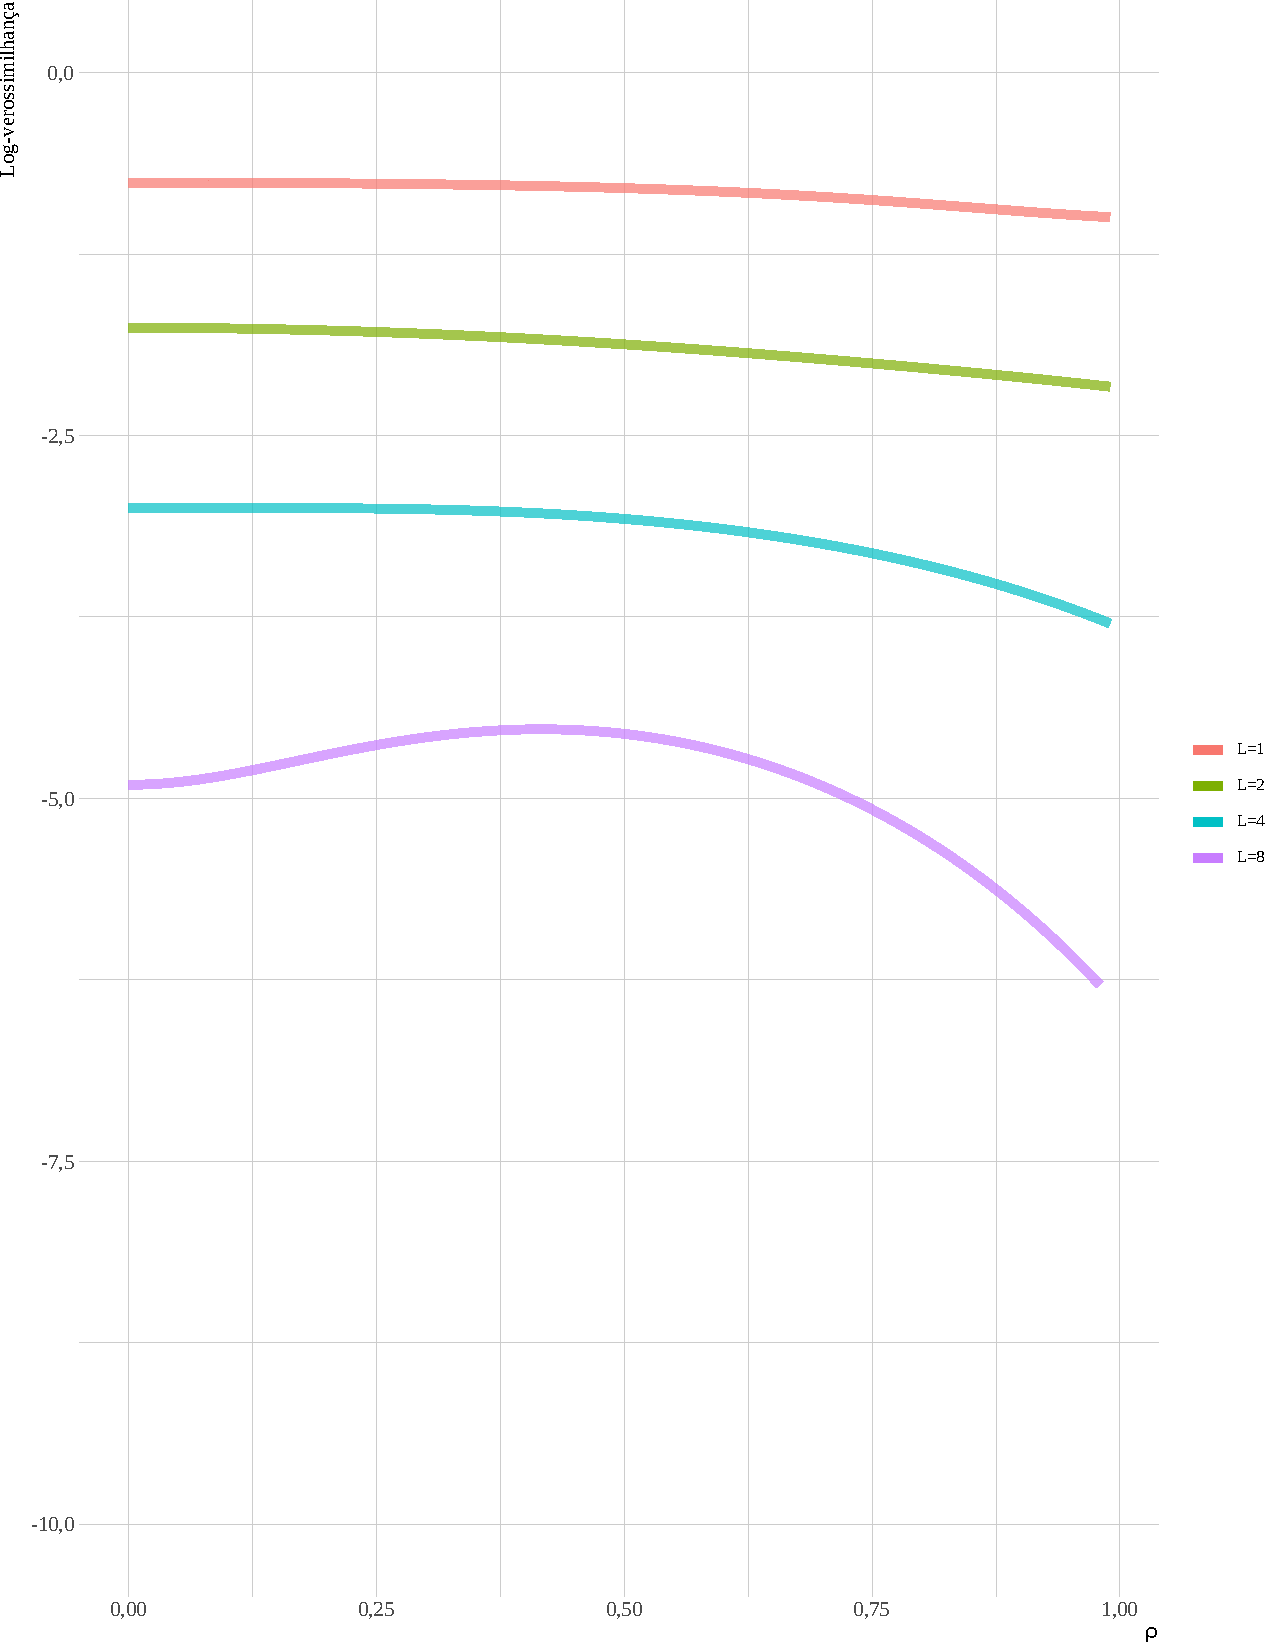
\includegraphics[width=0.32\linewidth]{log_like_prod_mag_L_fixo_por_150_to_400}}
     %\subfloat[Canal $\text{vv}$ \label{fig:evid_bordas_l:1c}]{%
     %  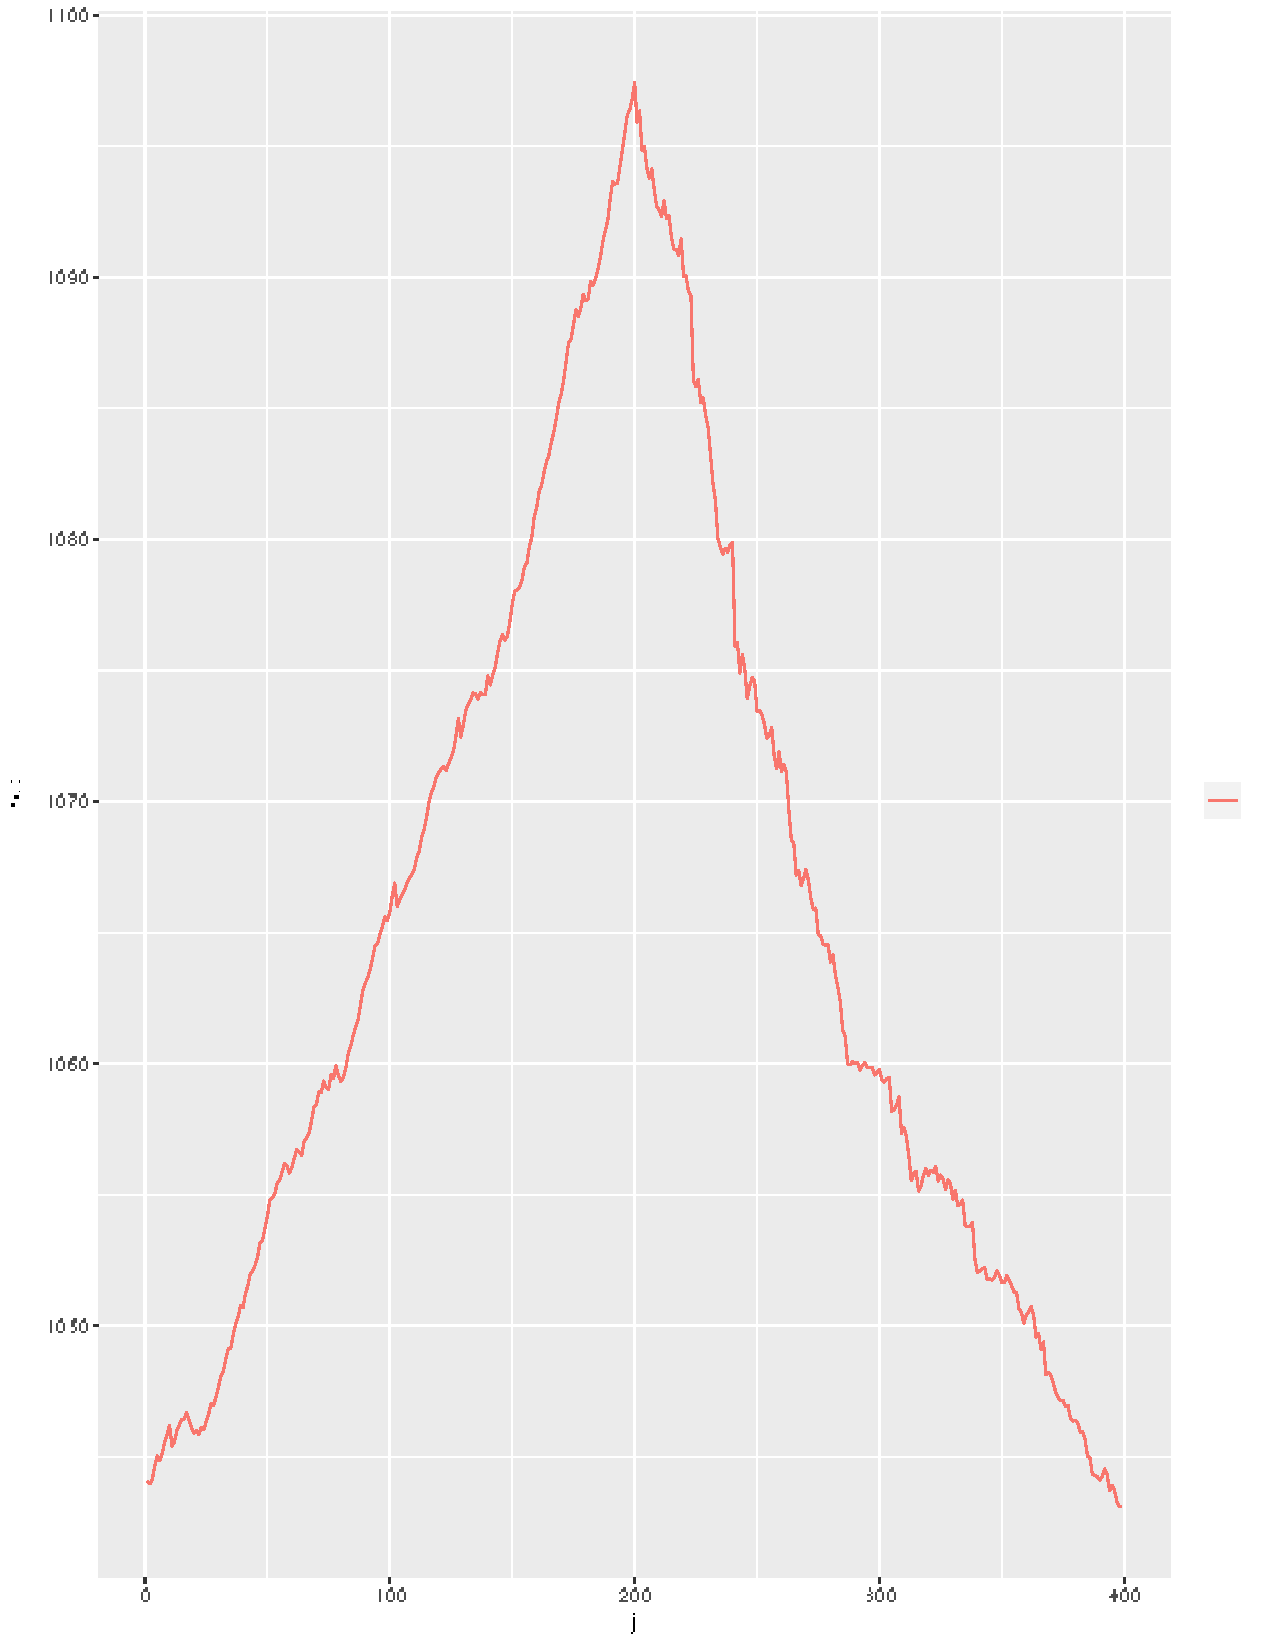
\includegraphics[width=0.32\linewidth]{grafico_l_gamf_2017_sigmahh_param_mu}}
     \caption{Distribuição produto de intensidades para diferentes L fixos e radial 35}
     \label{fig:pdf_prod_mag_flat}
   \end{figure}	


\subsubsection{Distribuição univariada razão de intensidades com L fixo}



    
\begin{figure}[hbt]
	\centering
     \subfloat[Canal $\text{hh}$ \label{fig:evid_bordas_l:1a}]{%
       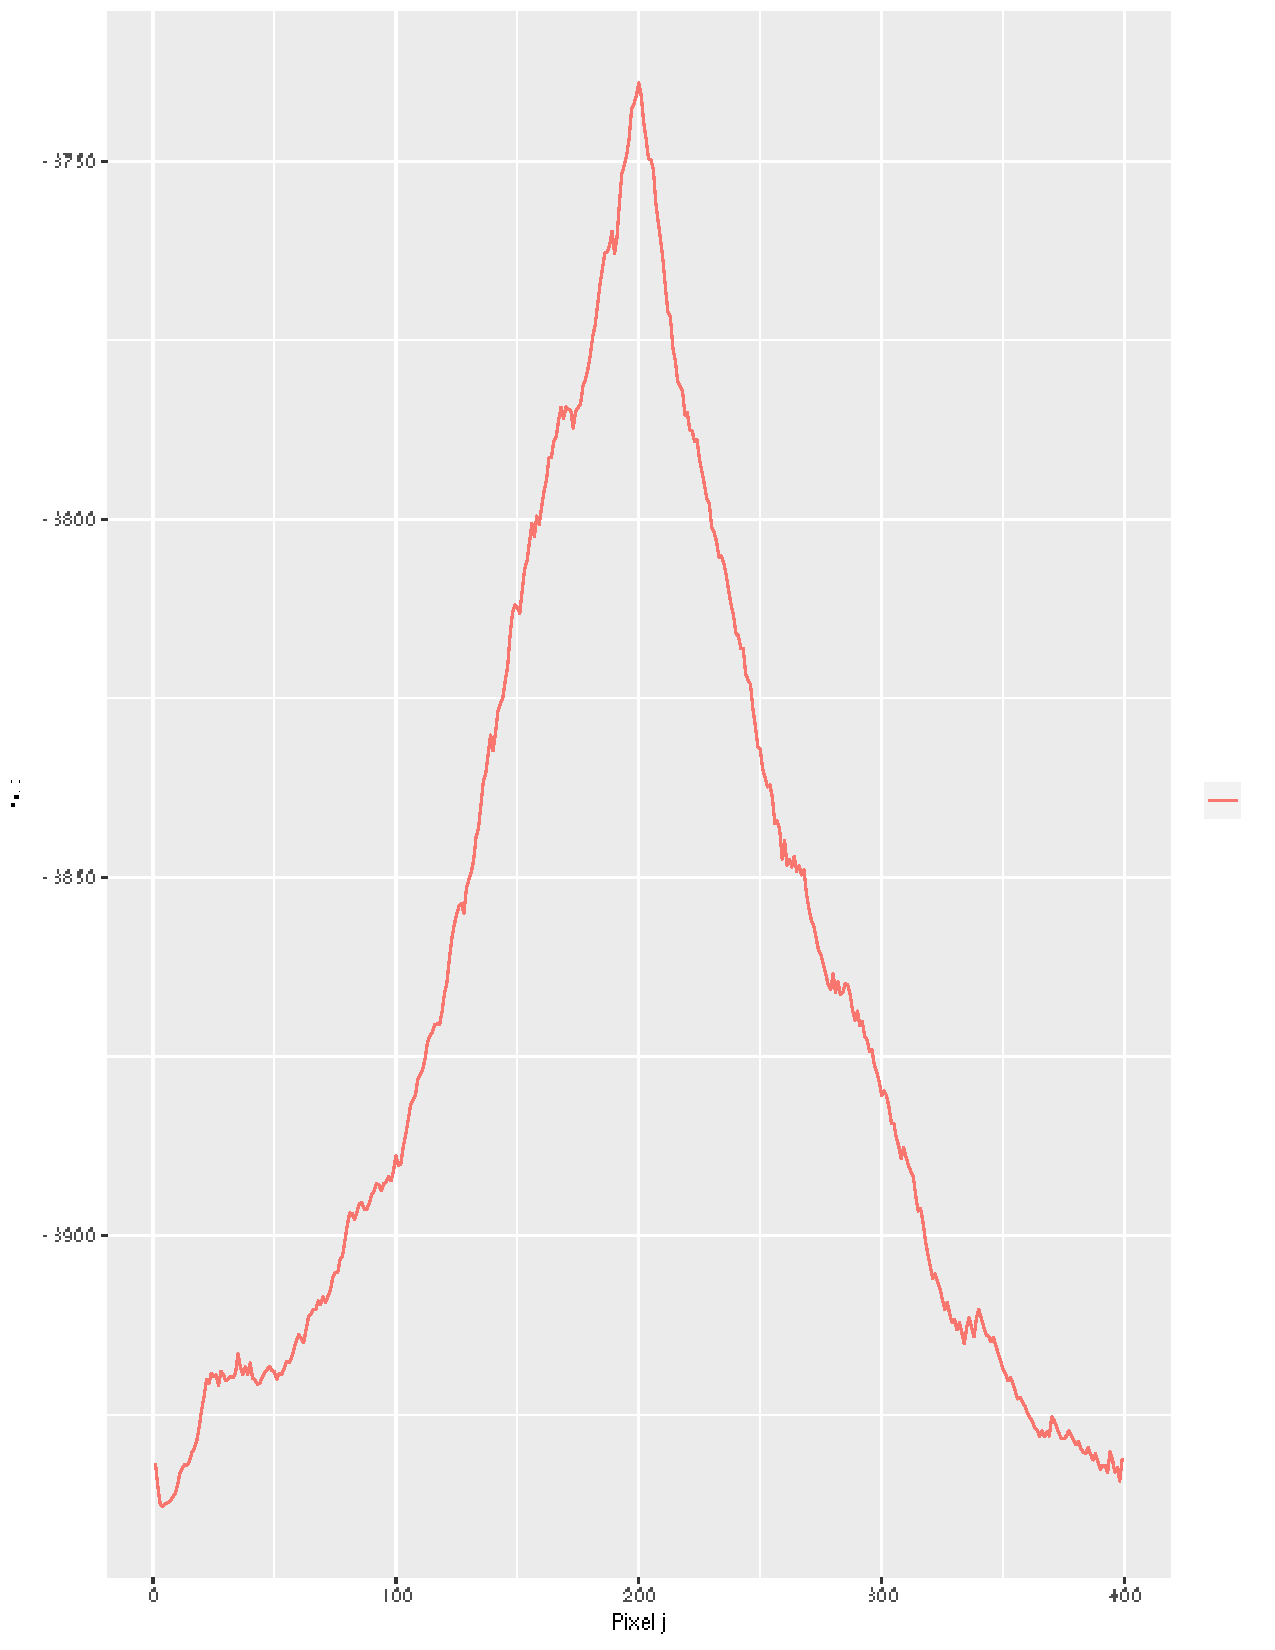
\includegraphics[width=0.32\linewidth]{grafico_l_gamf_razao_hh_hv_param_rho_tau}}
     \subfloat[Canal $\text{hv}$ \label{fig:evid_bordas_l:1b}]{%
       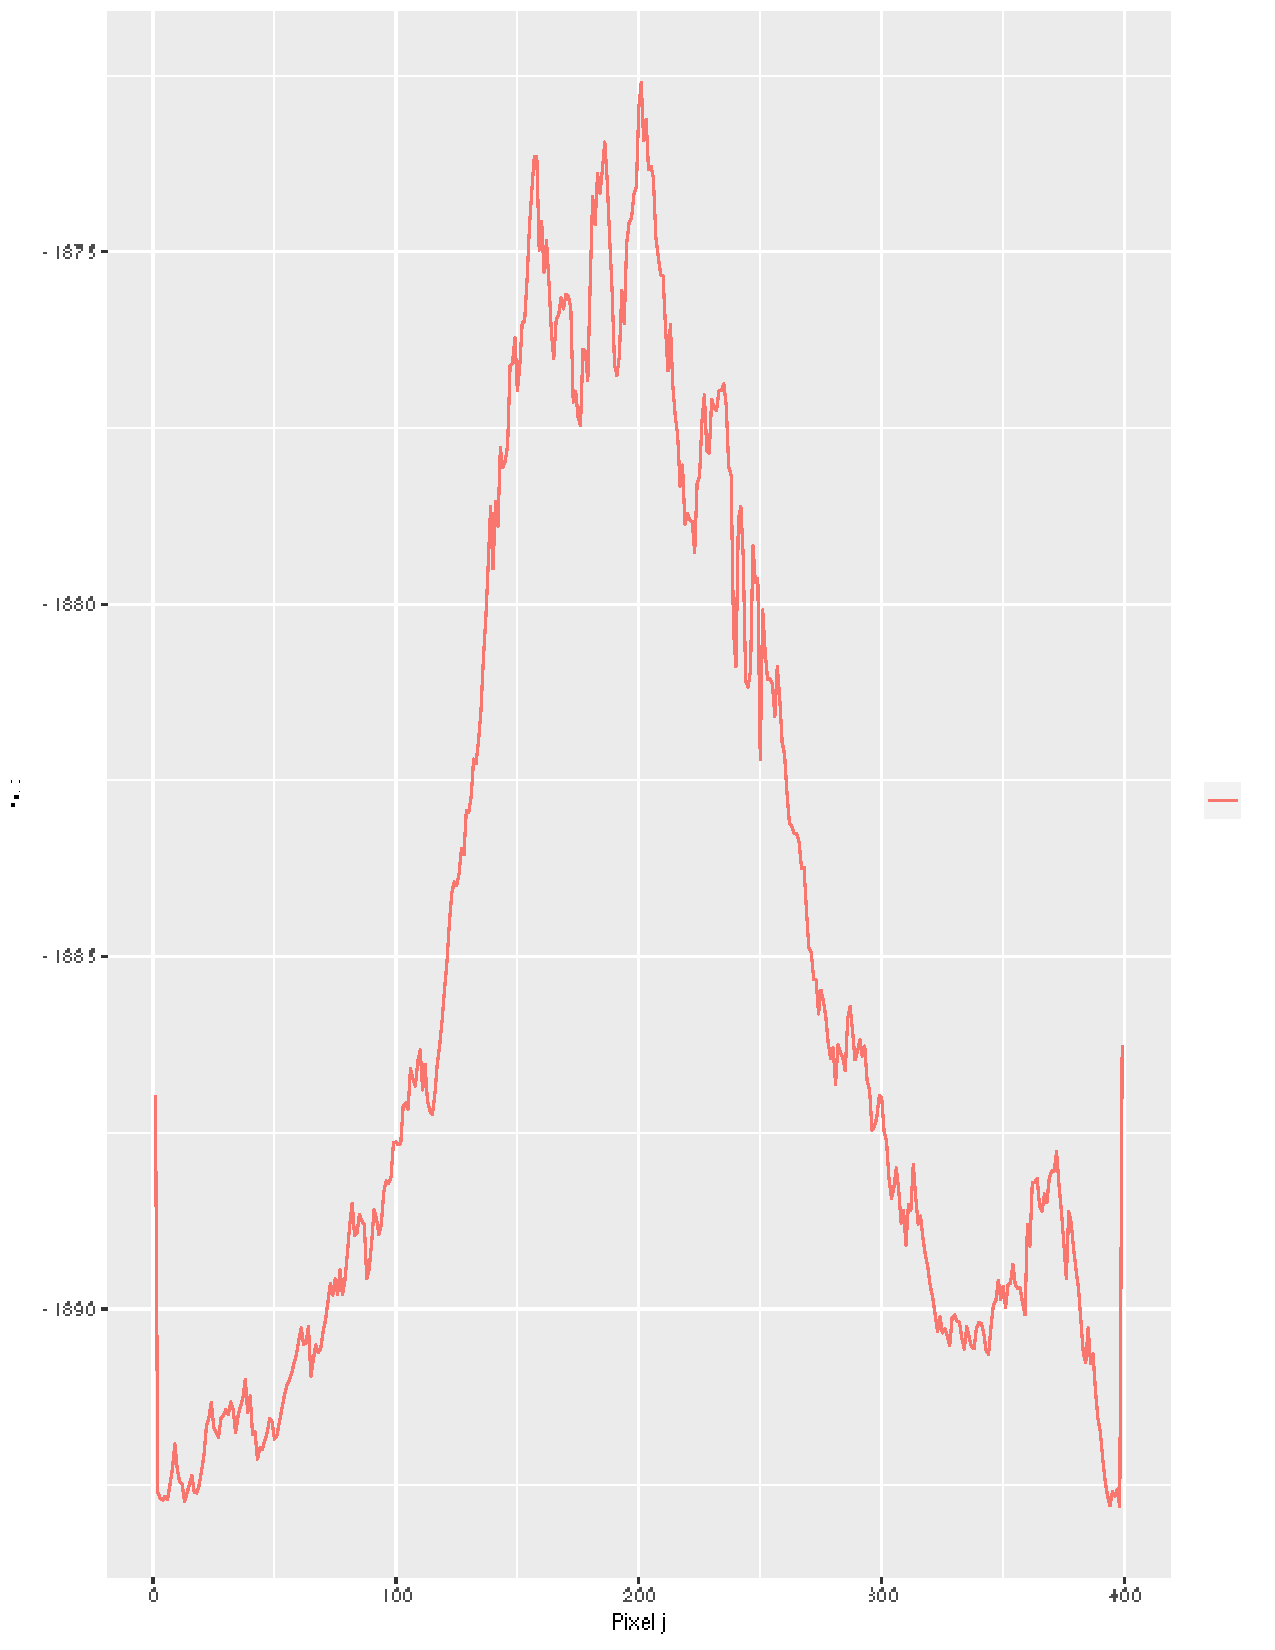
\includegraphics[width=0.32\linewidth]{grafico_l_gamf_razao_hh_vv_param_rho_tau}}
     \subfloat[Canal $\text{vv}$ \label{fig:evid_bordas_l:1c}]{%
       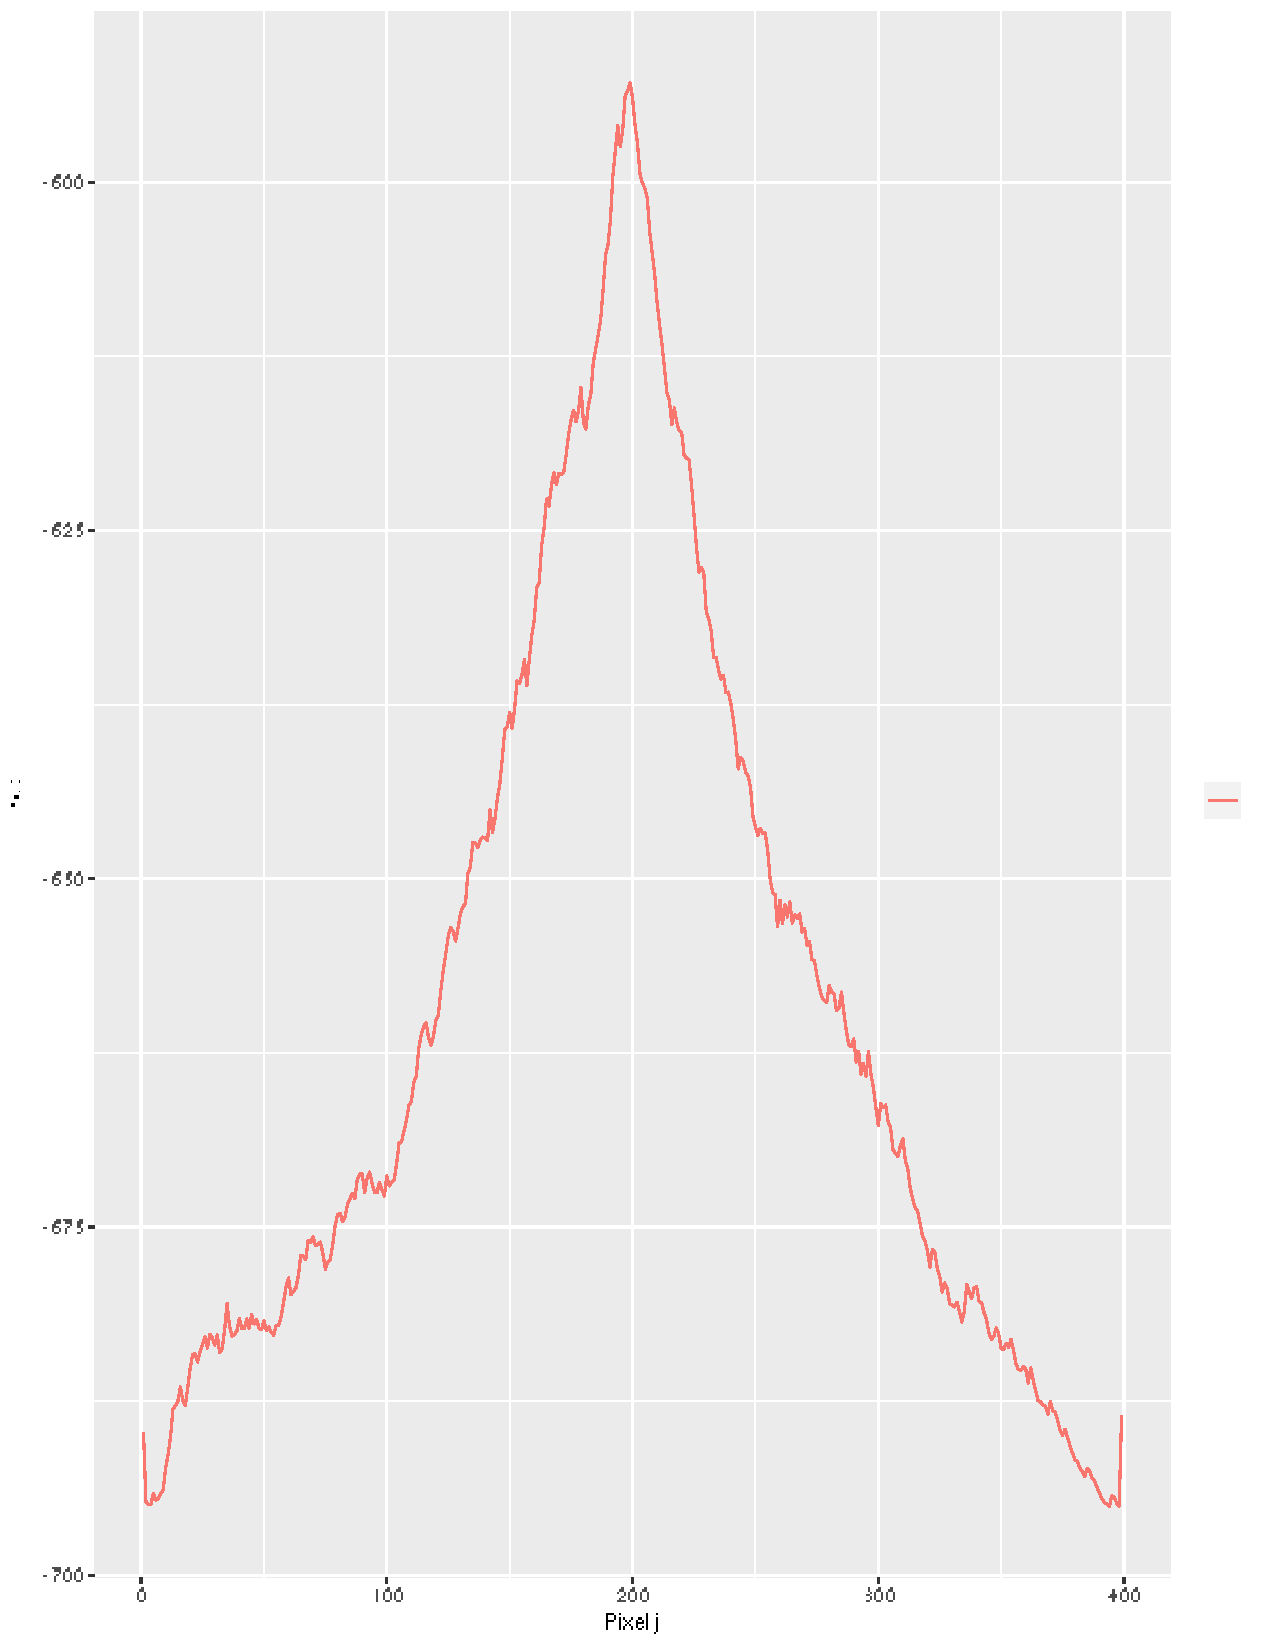
\includegraphics[width=0.32\linewidth]{grafico_l_gamf_razao_hv_vv_param_rho_tau}}
     \caption{Funções log-verossimilhanças para a radial 150}
     \label{fig:evid_bordas_l}
   \end{figure}	


\begin{figure*}[hbt]
	\centering
     \subfloat[Evidências no canal $\text{hh}$  \label{evidencias_hh_hv_vv_gamf_mu_estimado:a}]{%
       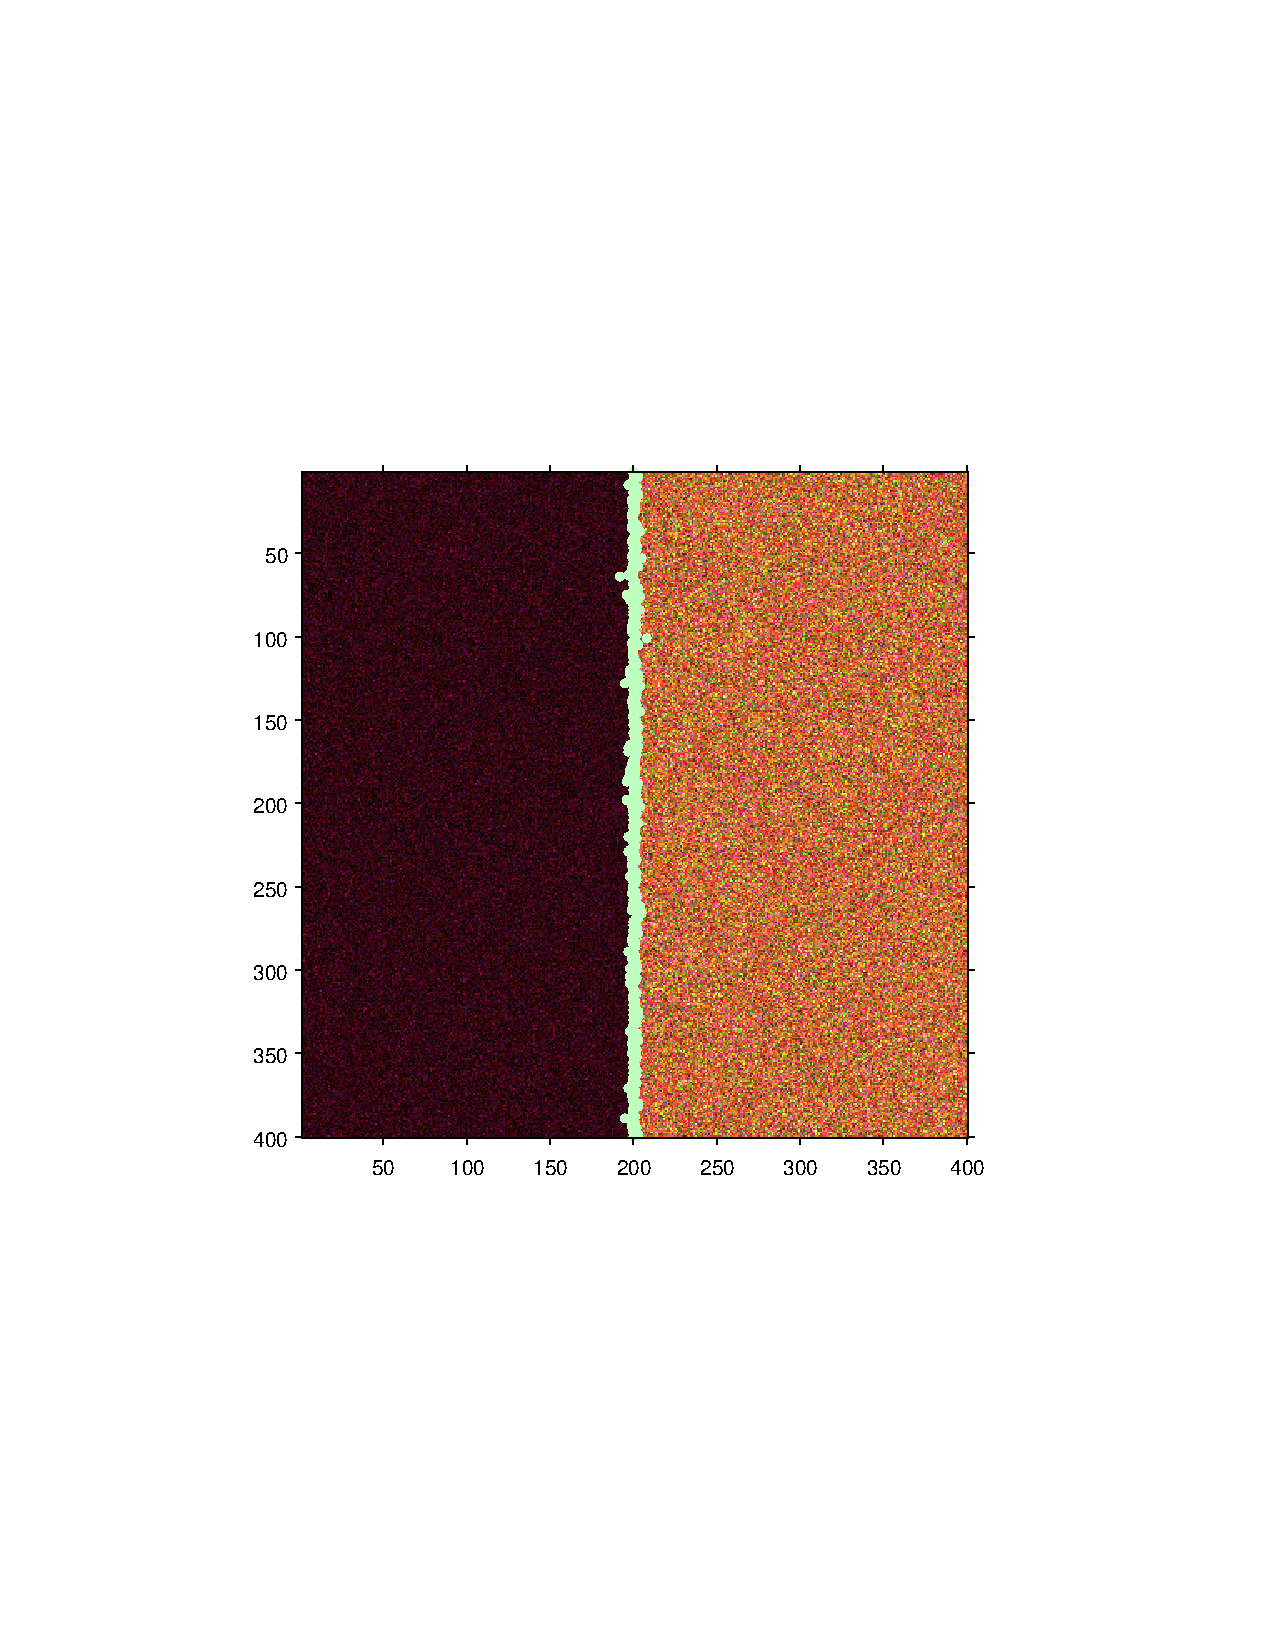
\includegraphics[width=0.35\linewidth]{im_sim_gamf_hh_hv_param_tau_rho_14_pixel}
     }
     \subfloat[Evidências no canal $\text{hv}$ \label{evidencias_hh_hv_vv_gamf_mu_estimado:b}]{%
       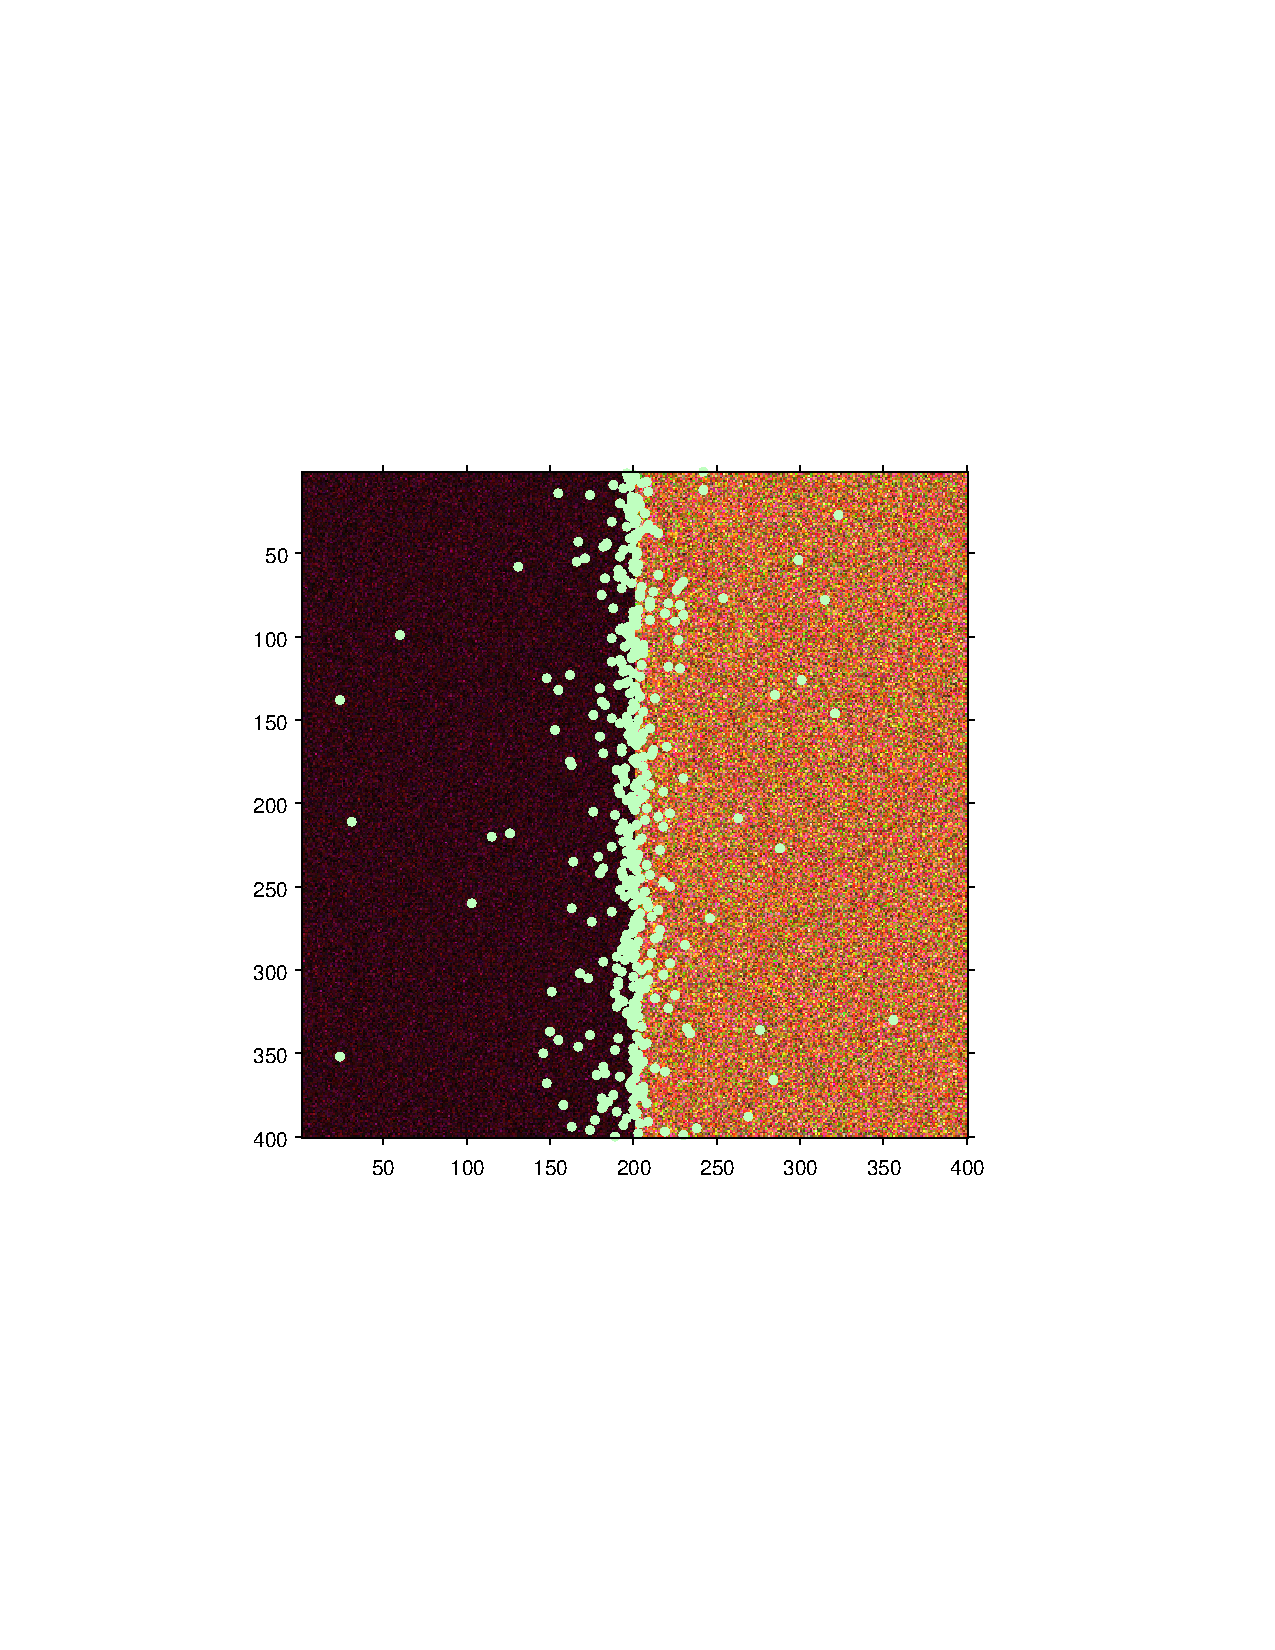
\includegraphics[width=0.35\linewidth]{im_sim_gamf_hh_vv_param_tau_rho_14_pixel}
     }      
     \subfloat[Evidências no canal $\text{vv}$ \label{evidencias_hh_hv_vv_gamf_mu_estimado:c}]{%
       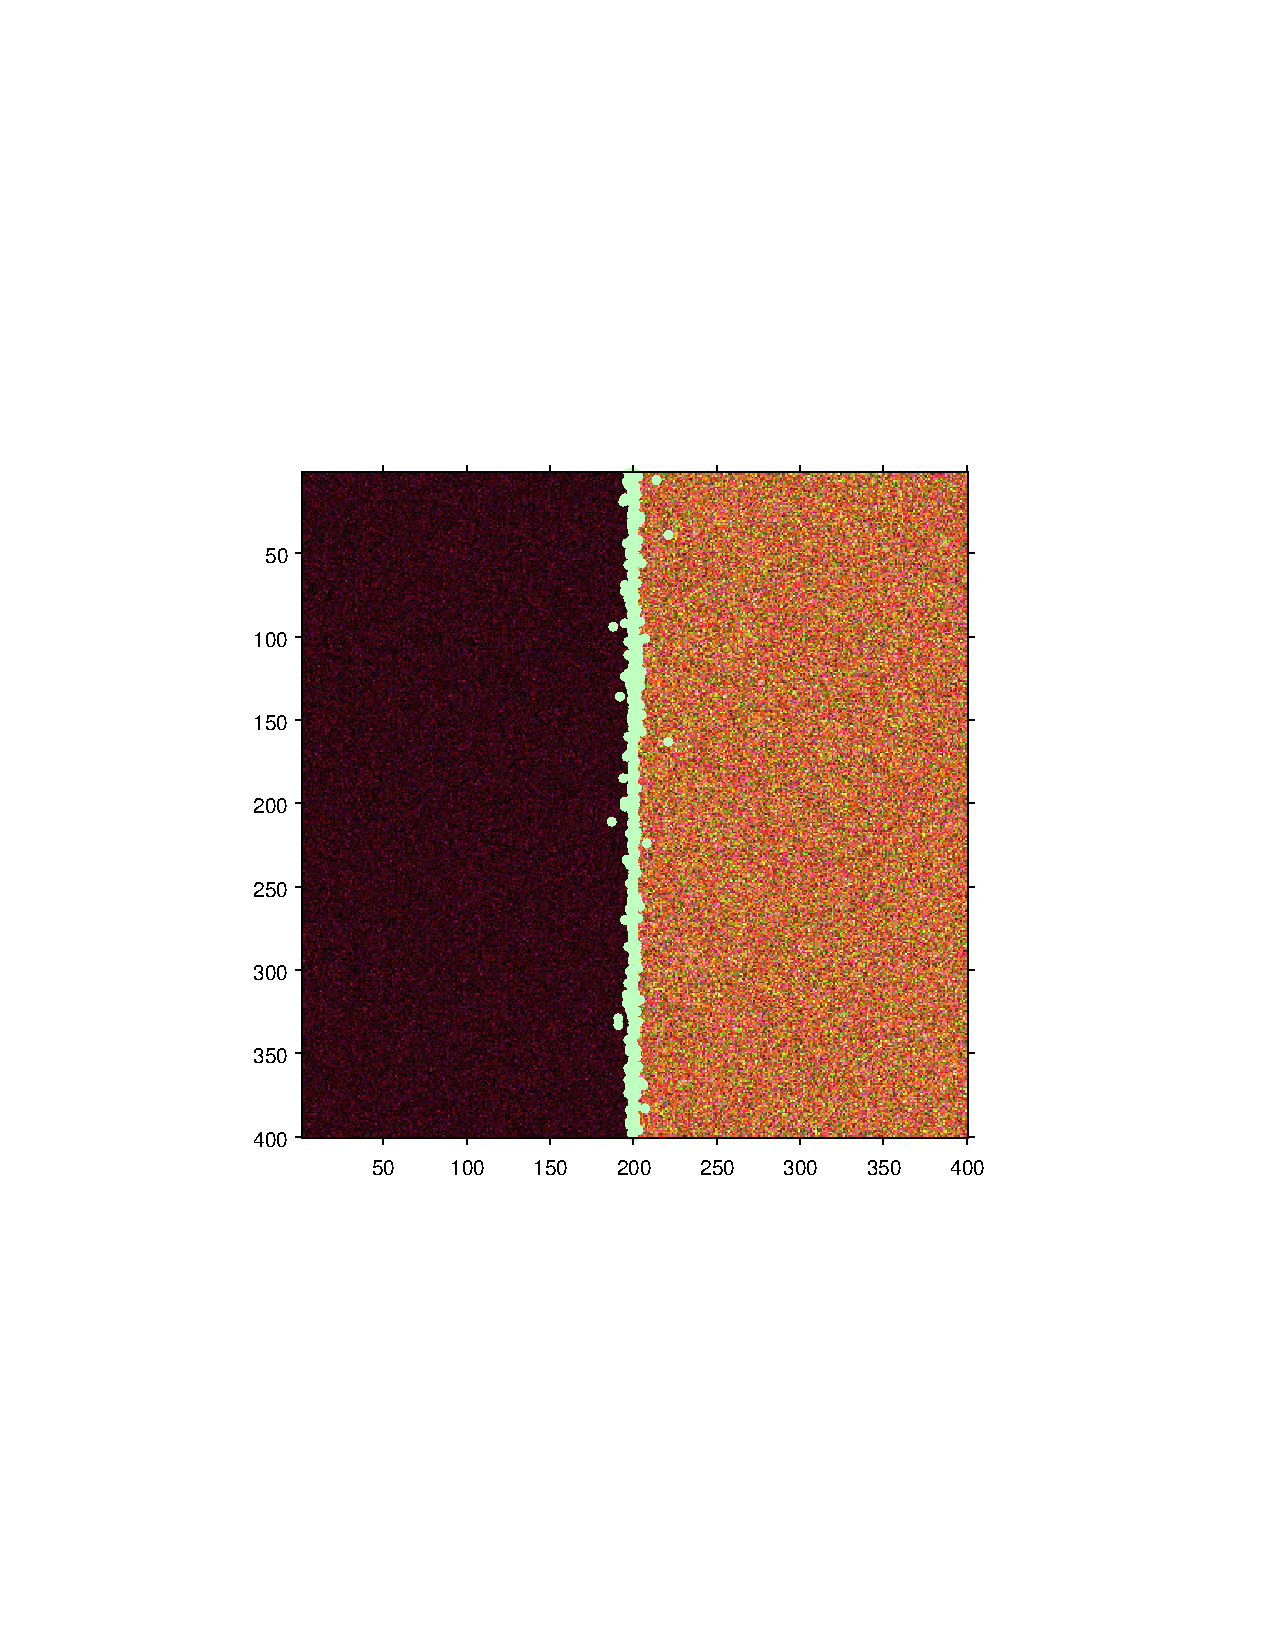
\includegraphics[width=0.35\linewidth]{im_sim_gamf_hv_vv_param_tau_rho_14_pixel}
     }
    \caption{Evidências de bordas para os três canais de intensidade com $\mu$ estimado.}
     \label{evidencias_hh_hv_vv_gamf} 
   \end{figure*}


\subsubsection{Distribuição bivariada produto de intensidades com L fixo}

%\begin{figure}[hbt]
%	\centering
%     \subfloat[Canal $\text{hh}$ \label{fig:evid_bordas_l:1a}]{%
%       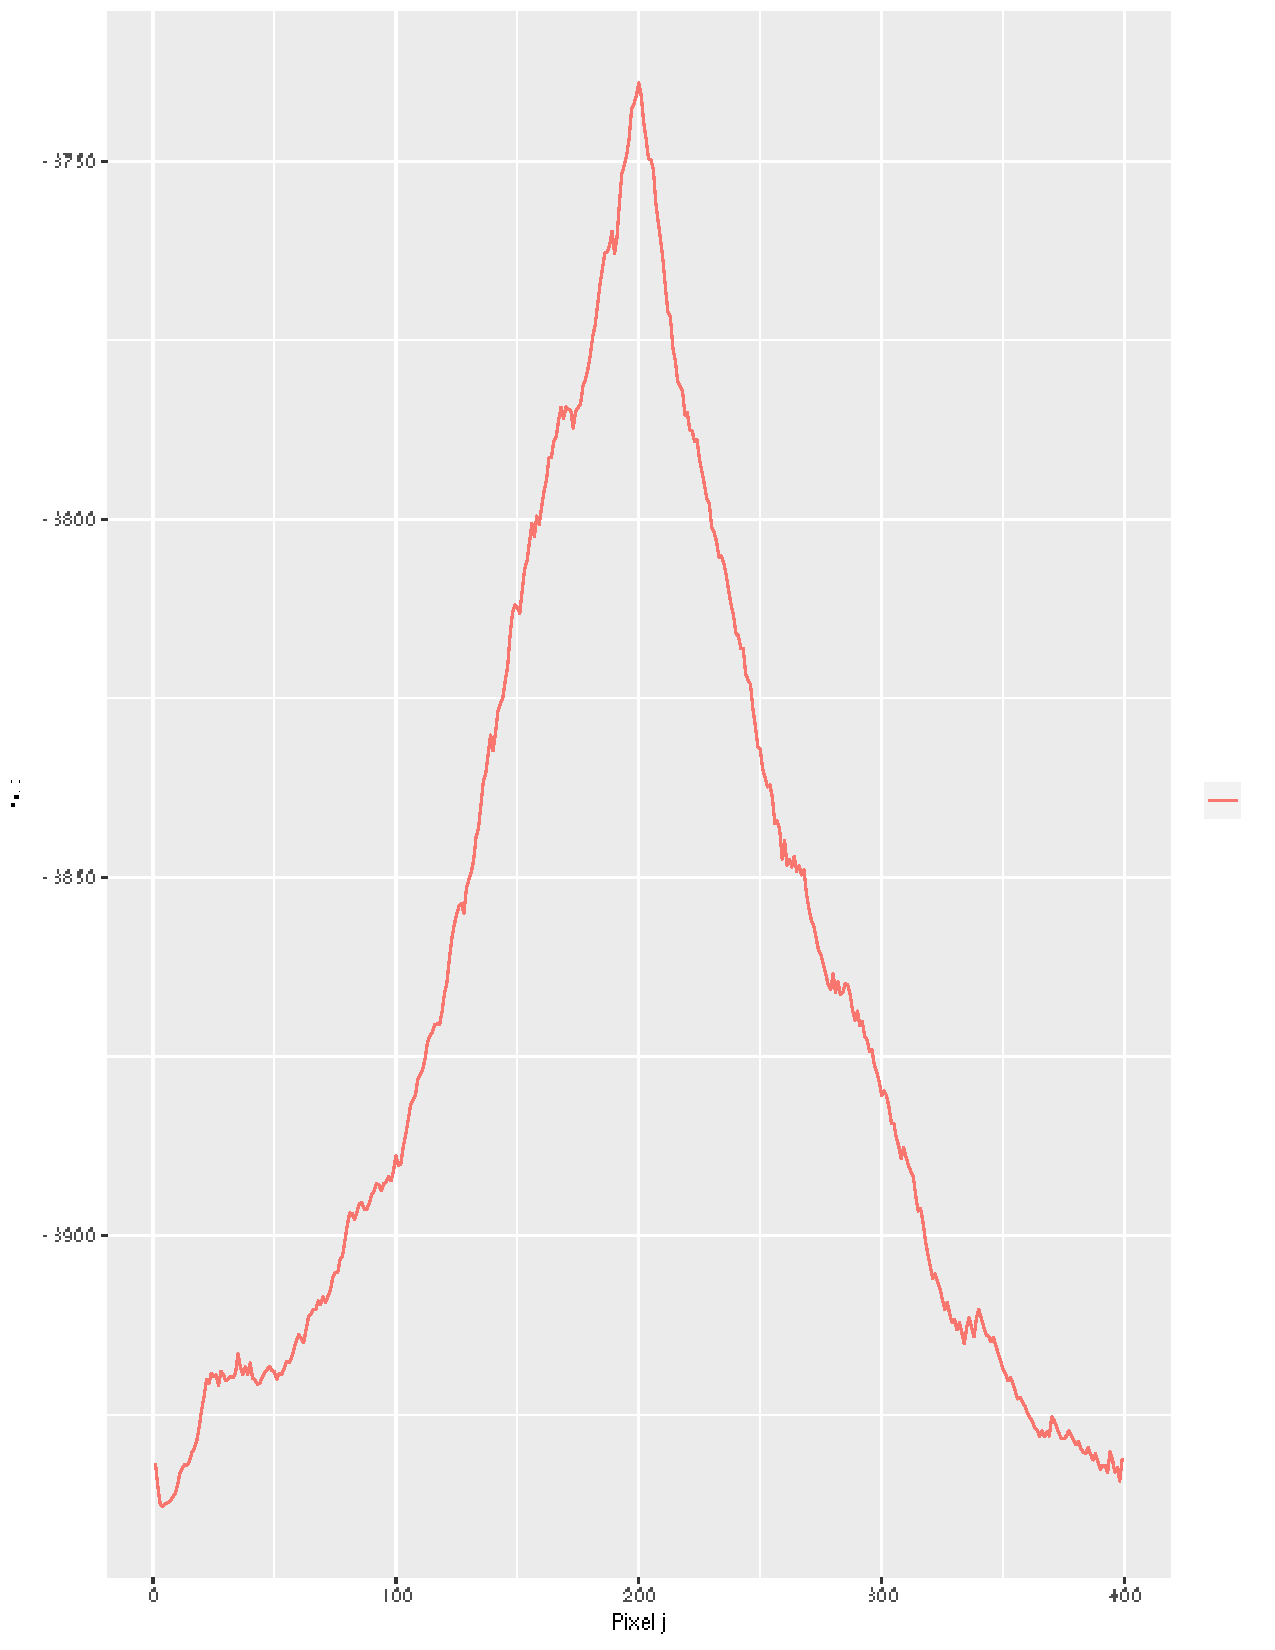
\includegraphics[width=0.32\linewidth]{grafico_l_gamf_razao_hh_hv_param_rho_tau}}
%     \subfloat[Canal $\text{hv}$ \label{fig:evid_bordas_l:1b}]{%
%       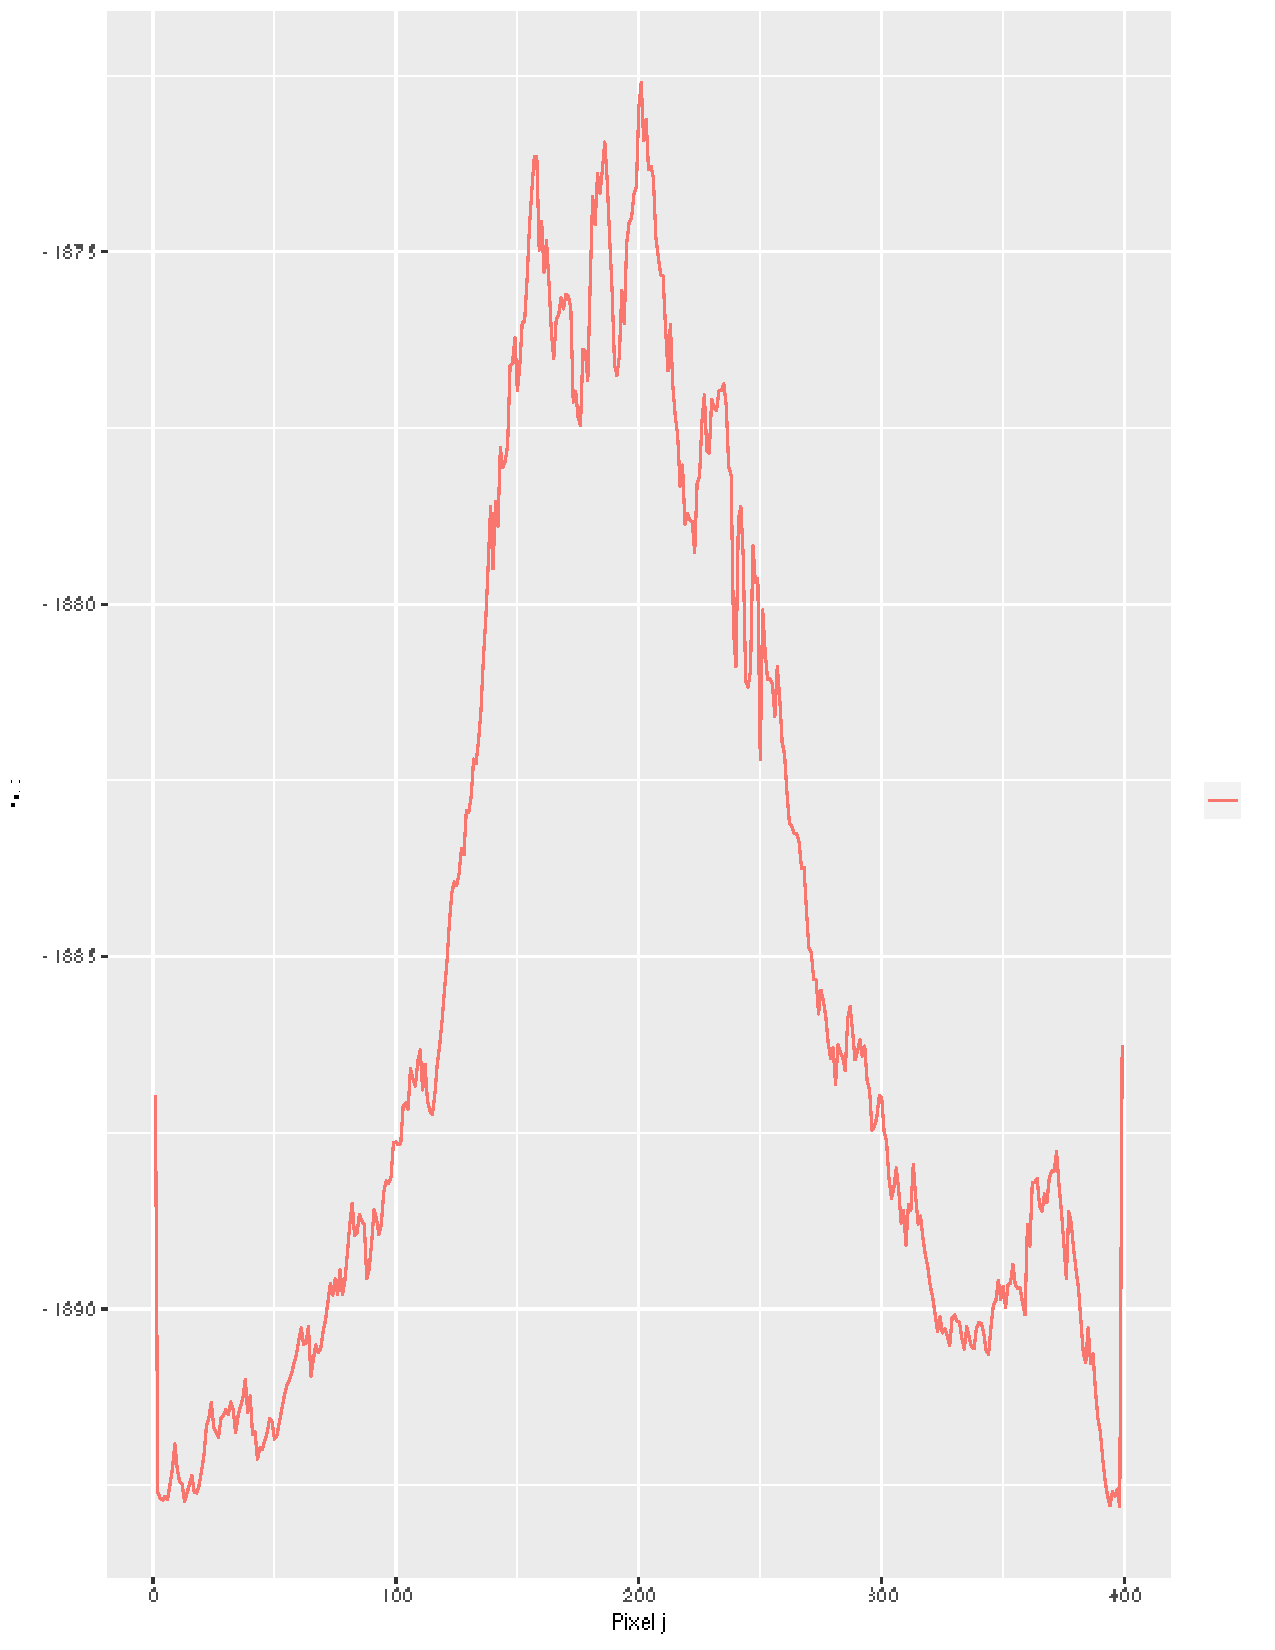
\includegraphics[width=0.32\linewidth]{grafico_l_gamf_razao_hh_vv_param_rho_tau}}
%     \subfloat[Canal $\text{vv}$ \label{fig:evid_bordas_l:1c}]{%
%       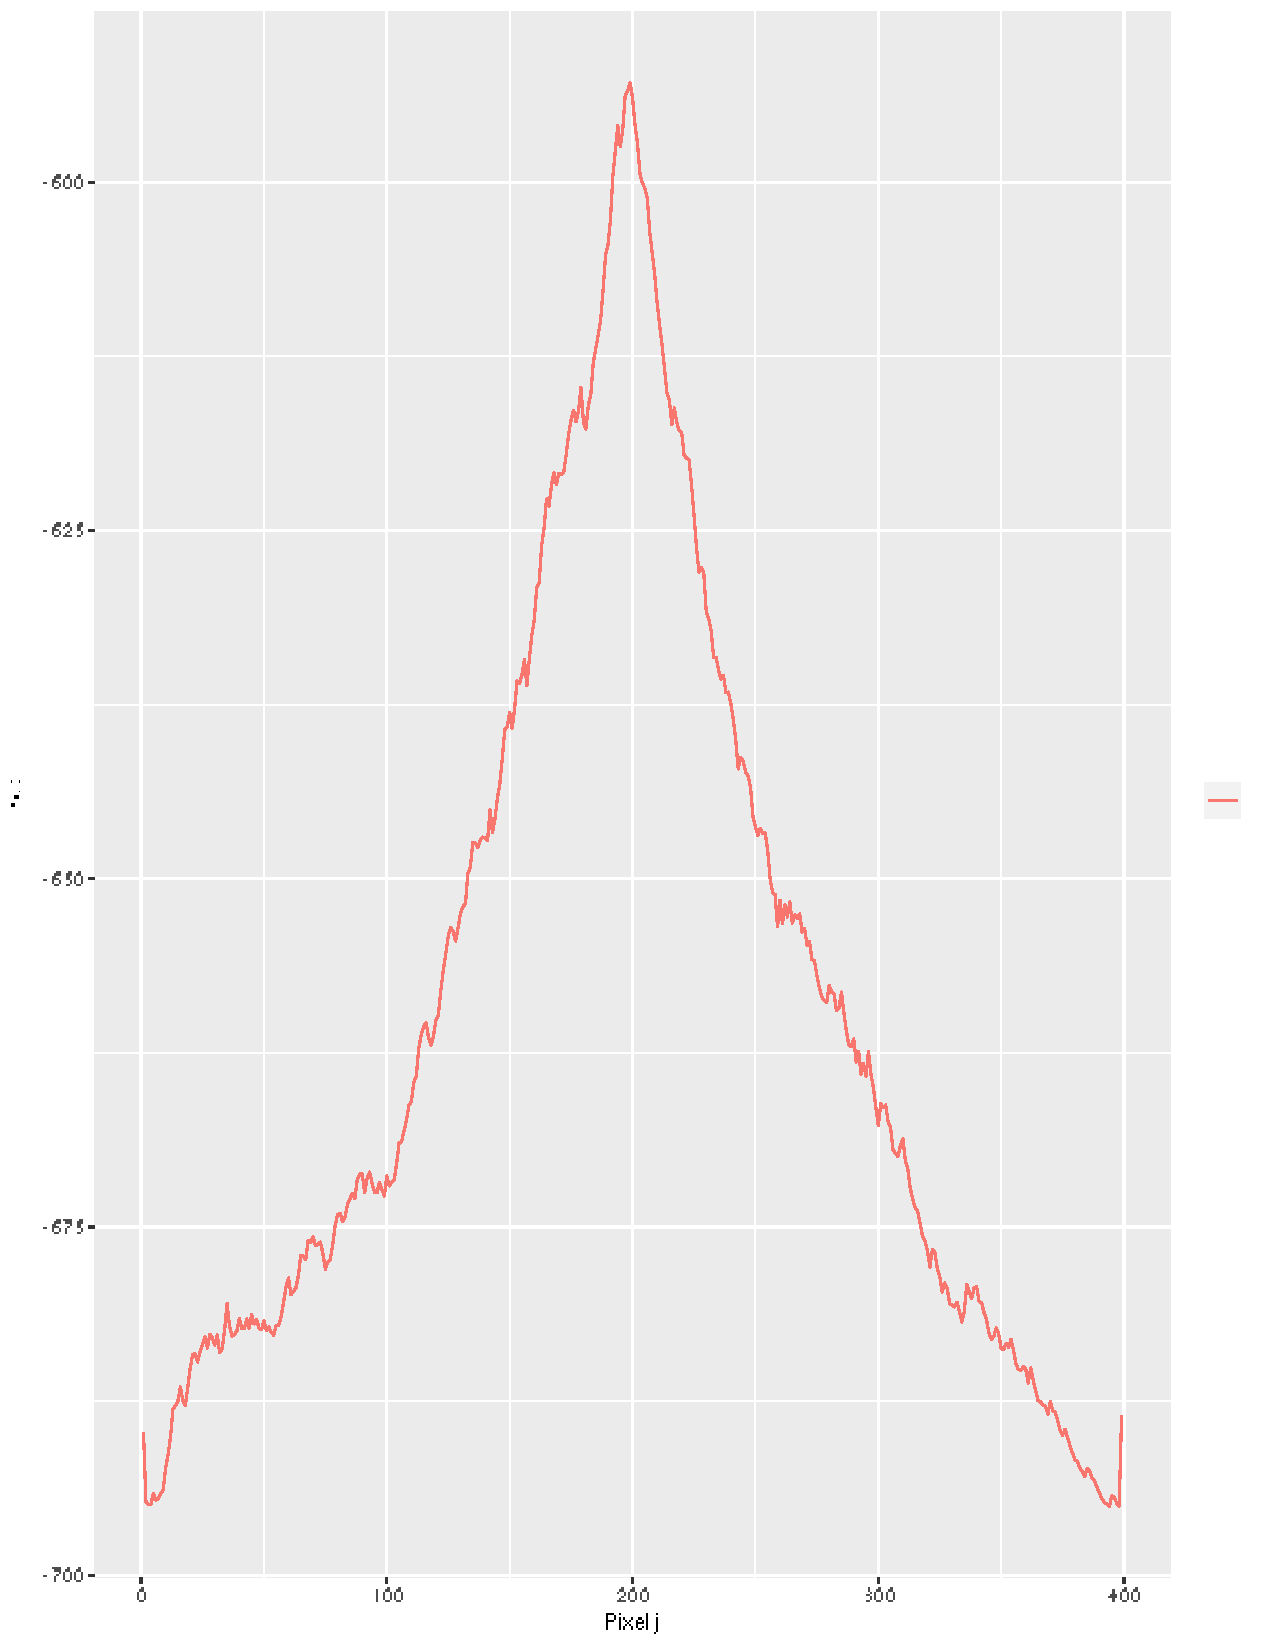
\includegraphics[width=0.32\linewidth]{grafico_l_gamf_razao_hv_vv_param_rho_tau}}
%     \caption{Funções log-verossimilhanças para a radial 150}
%     \label{fig:evid_bordas_l}
%   \end{figure}	
%
%
%\begin{figure*}[hbt]
%	\centering
%     \subfloat[Evidências no canal $\text{hh}$  \label{evidencias_hh_hv_vv_gamf_mu_estimado:a}]{%
%       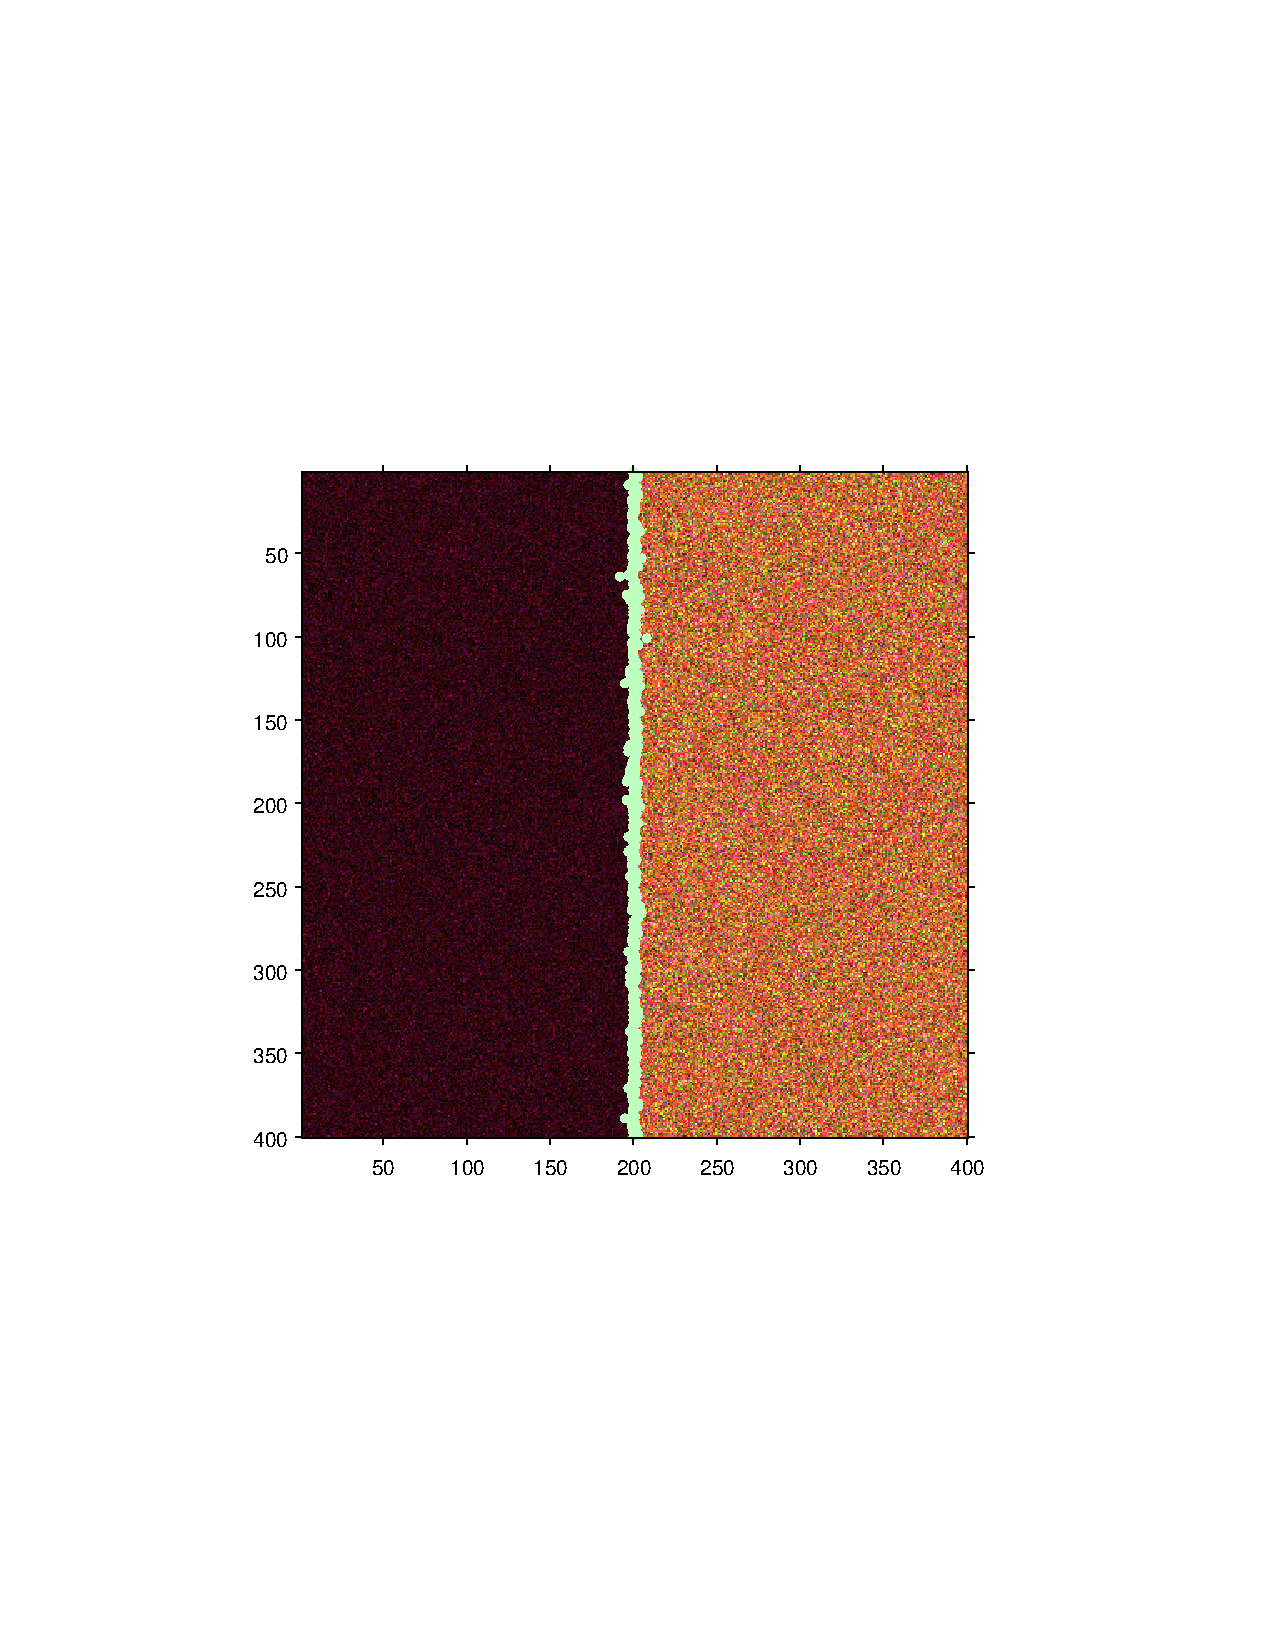
\includegraphics[width=0.35\linewidth]{im_sim_gamf_hh_hv_param_tau_rho_14_pixel}
%     }
%     \subfloat[Evidências no canal $\text{hv}$ \label{evidencias_hh_hv_vv_gamf_mu_estimado:b}]{%
%       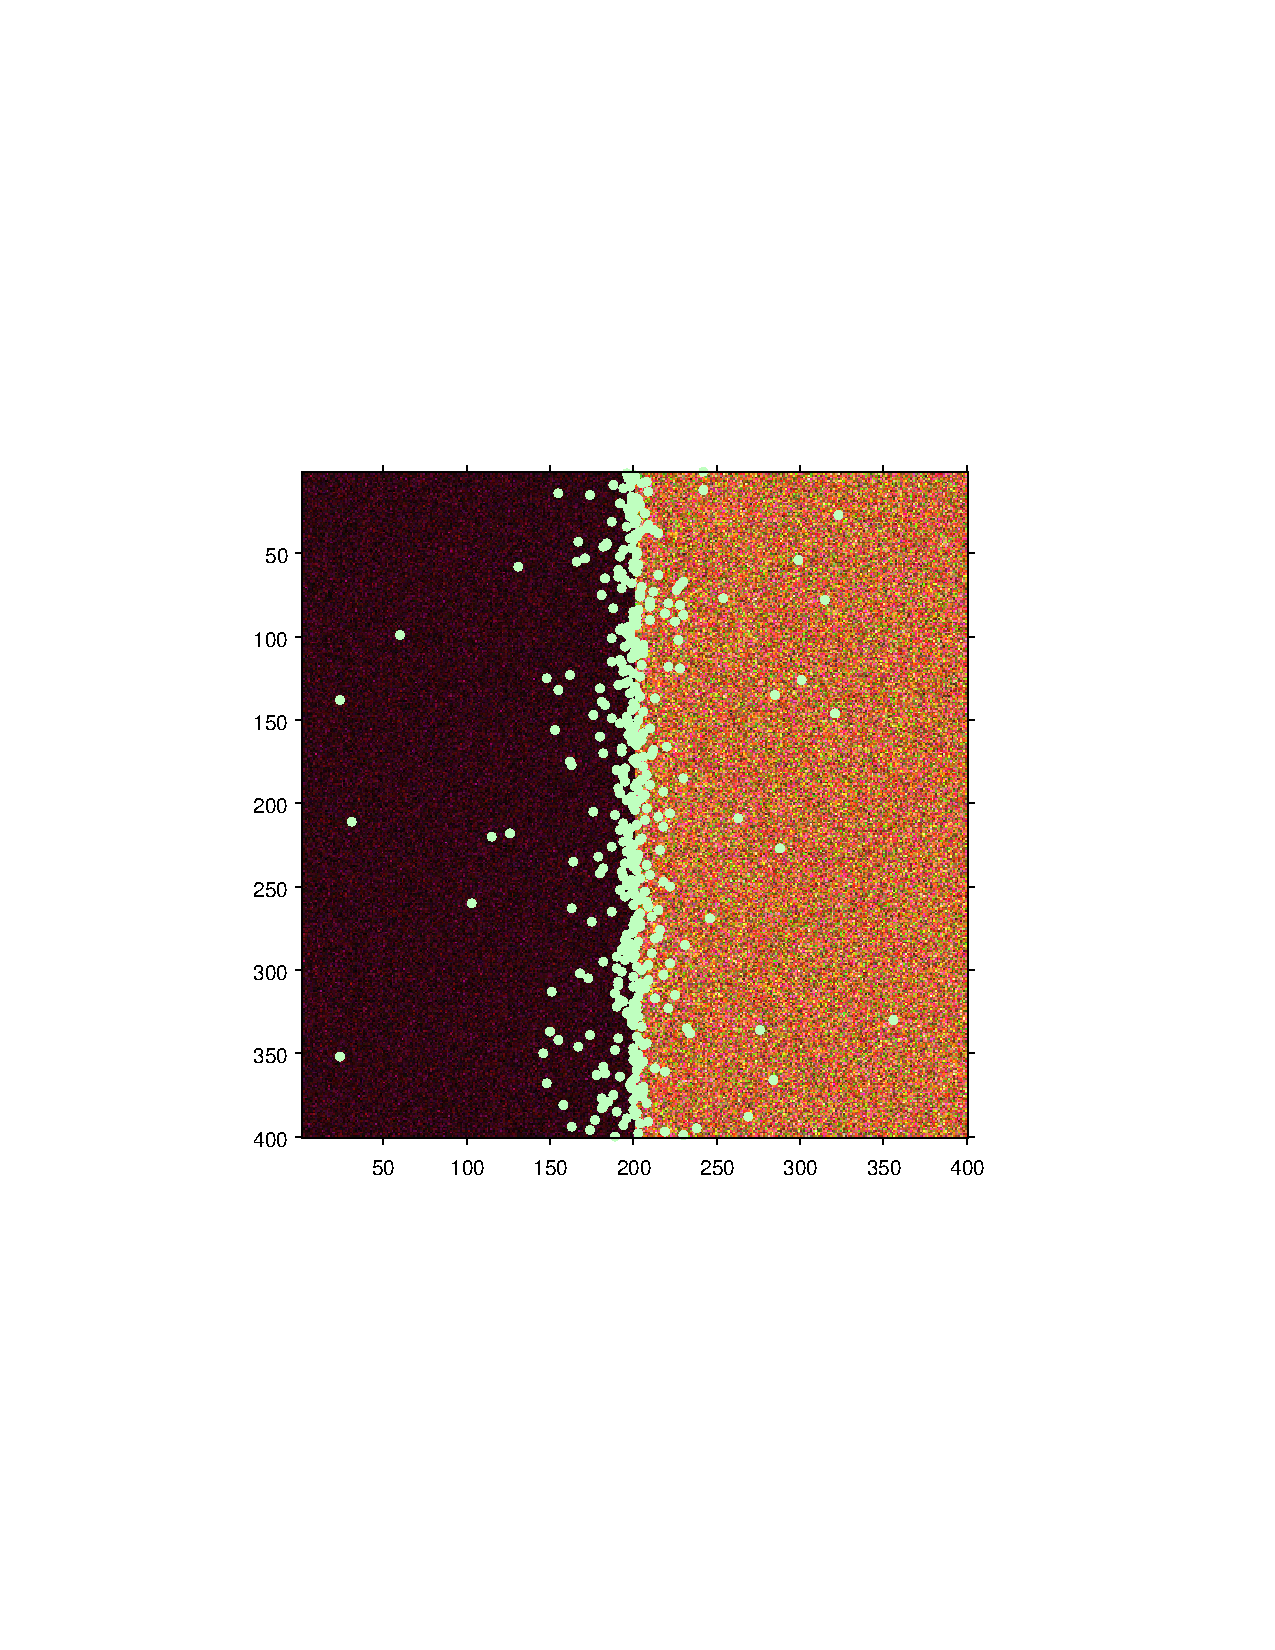
\includegraphics[width=0.35\linewidth]{im_sim_gamf_hh_vv_param_tau_rho_14_pixel}
%     }      
%     \subfloat[Evidências no canal $\text{vv}$ \label{evidencias_hh_hv_vv_gamf_mu_estimado:c}]{%
%       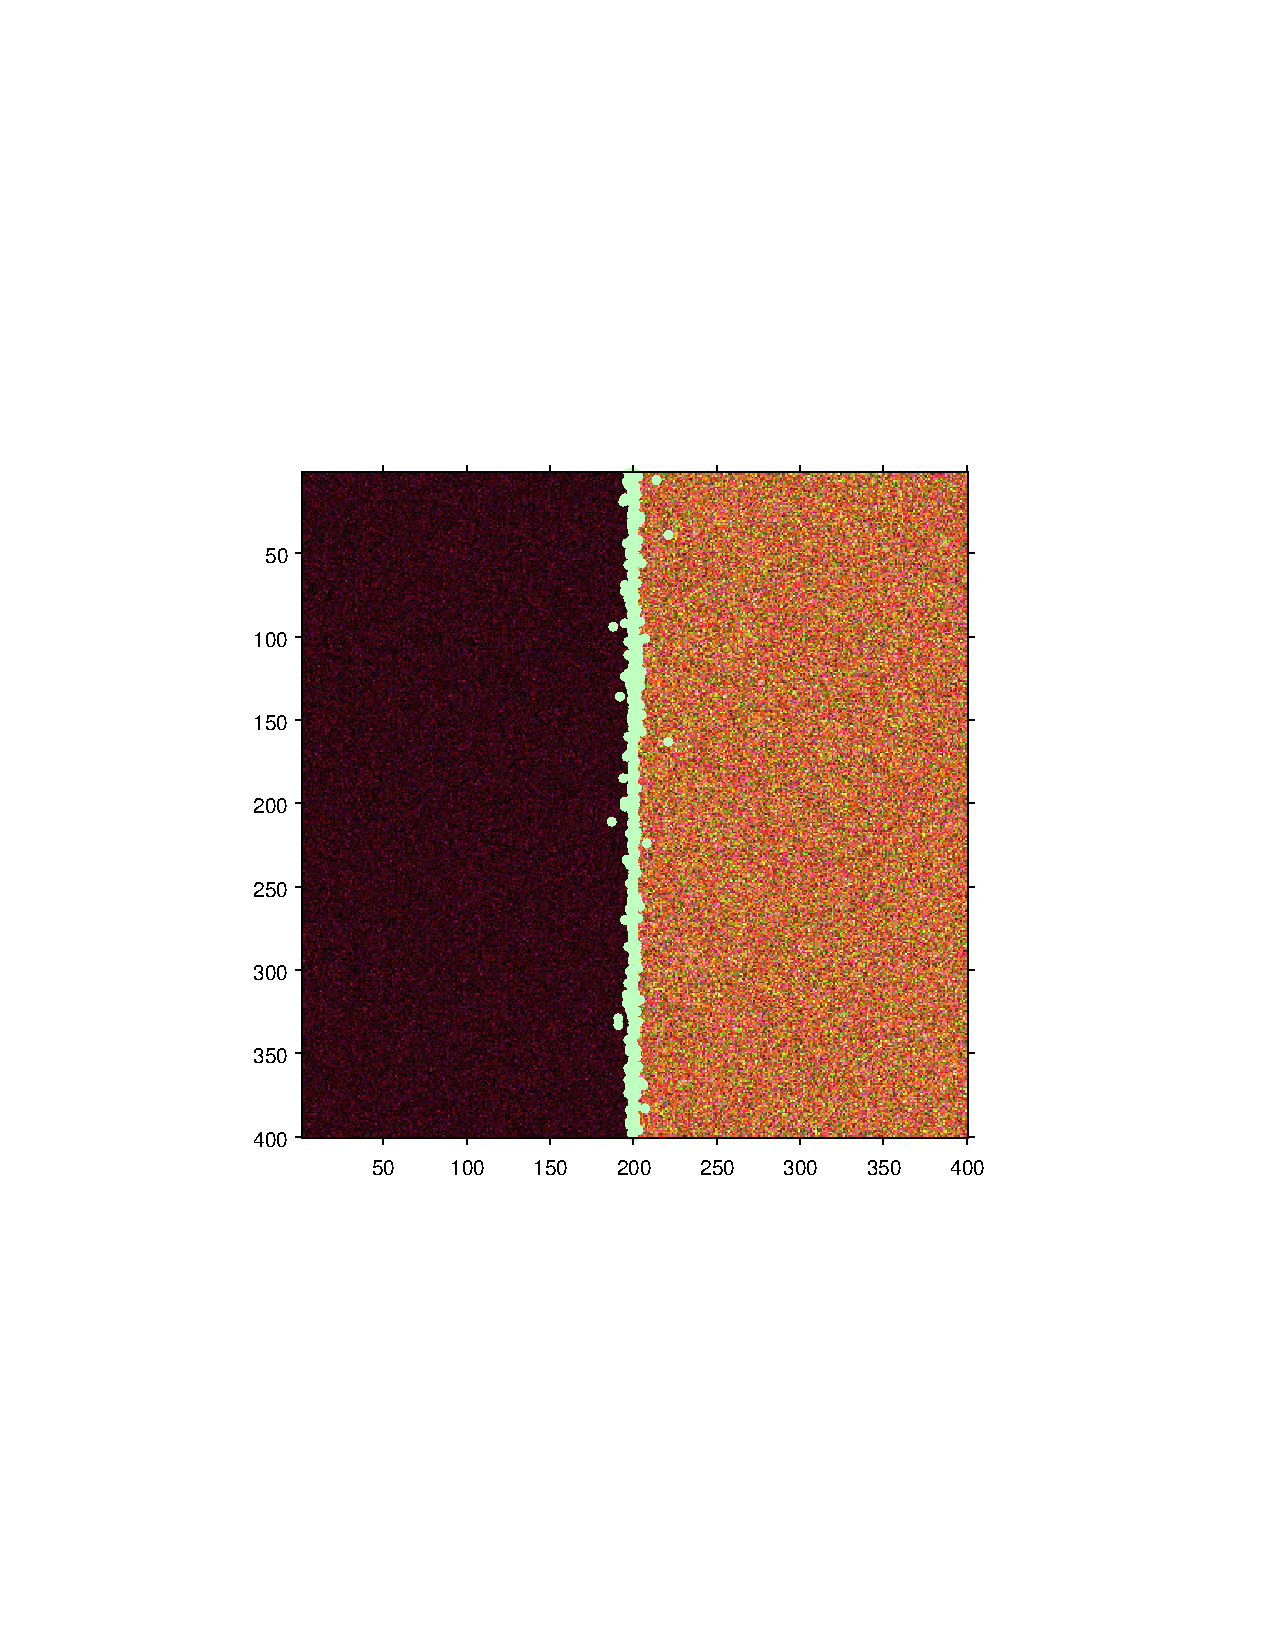
\includegraphics[width=0.35\linewidth]{im_sim_gamf_hv_vv_param_tau_rho_14_pixel}
%     }
%    \caption{Evidências de bordas para os três canais de intensidade com $\mu$ estimado.}
%     \label{evidencias_hh_hv_vv_gamf} 
%   \end{figure*}    
    
\subsubsection{Distribuição univariada span com L fixo}    
    
\begin{figure}[hbt]
	\centering
	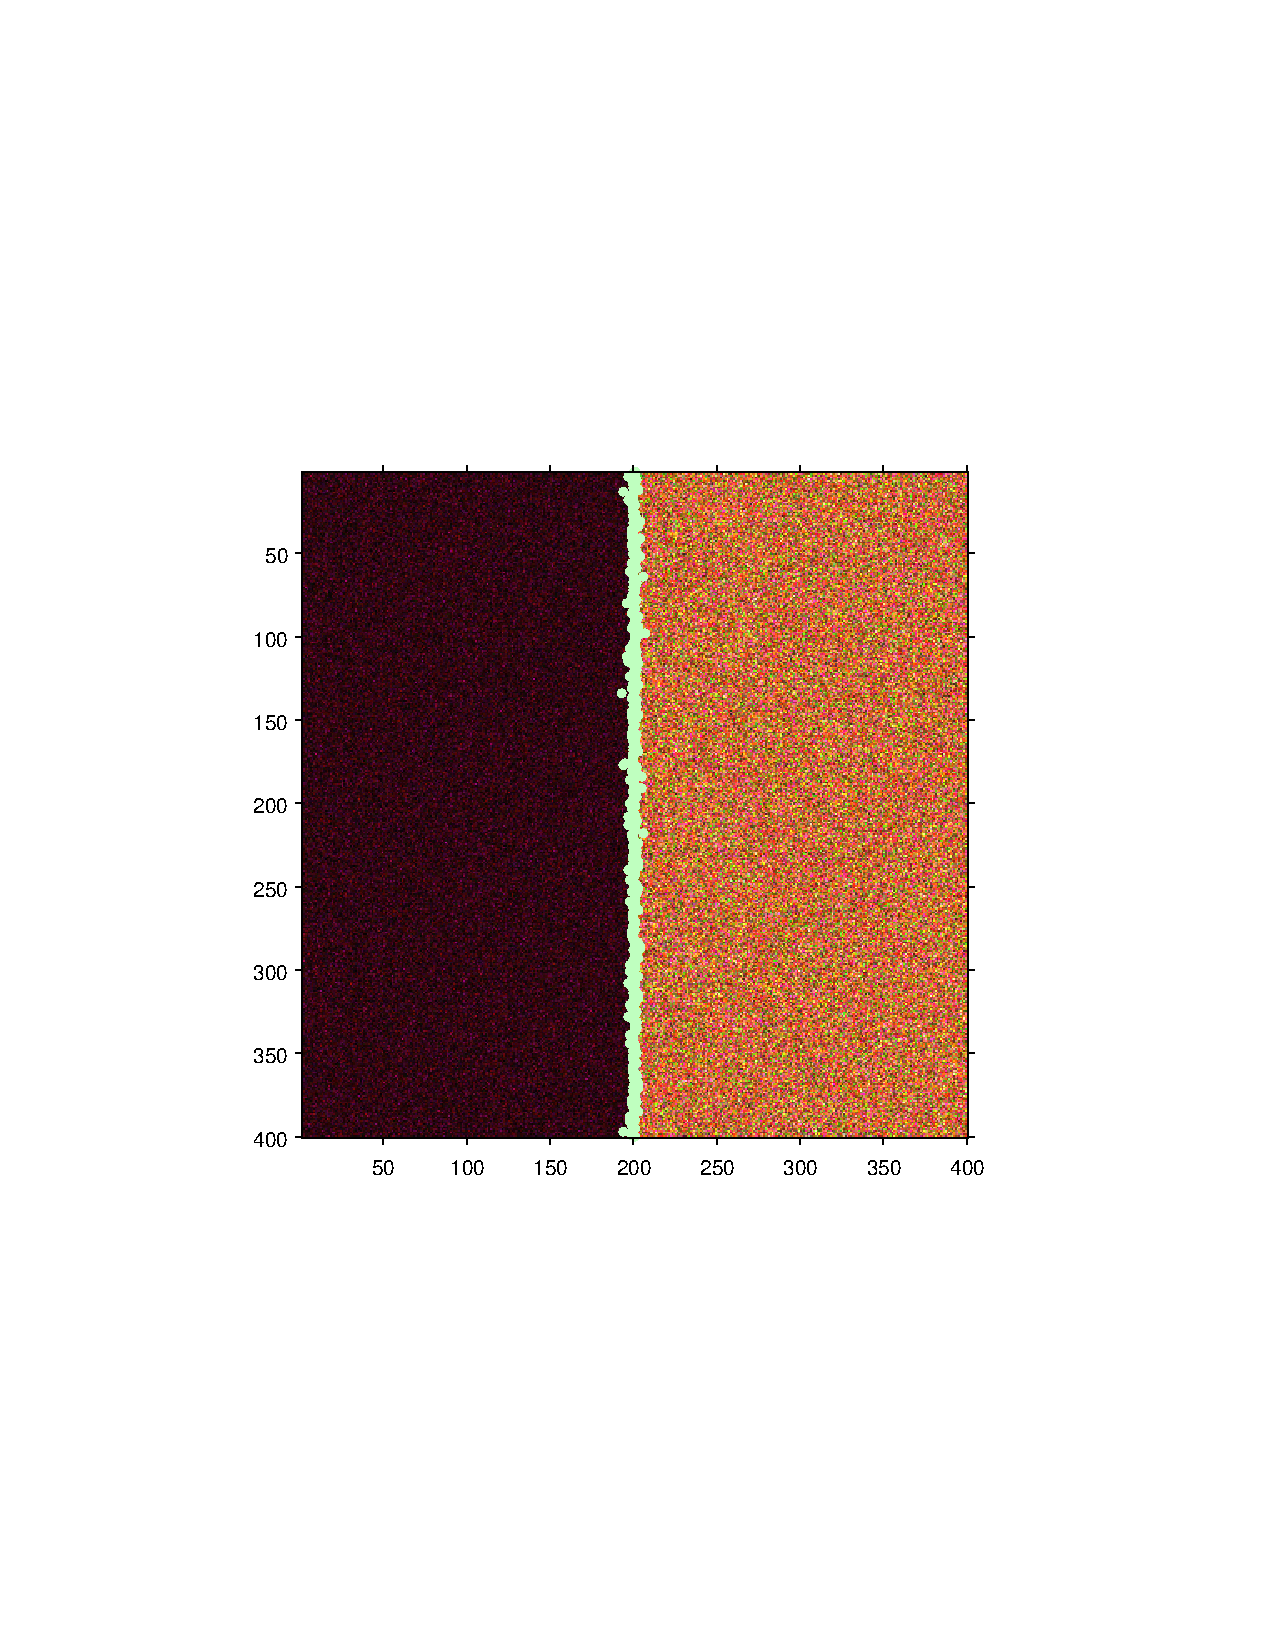
\includegraphics[width=.7\linewidth]{im_sim_gamf_span_param_mu_14_pixel}%
	\caption{Evidências de bordas para o span}
\label{fig:evidencias_span_gamf}
\end{figure}
    
    
    
\begin{figure}[hbt]
	\centering
	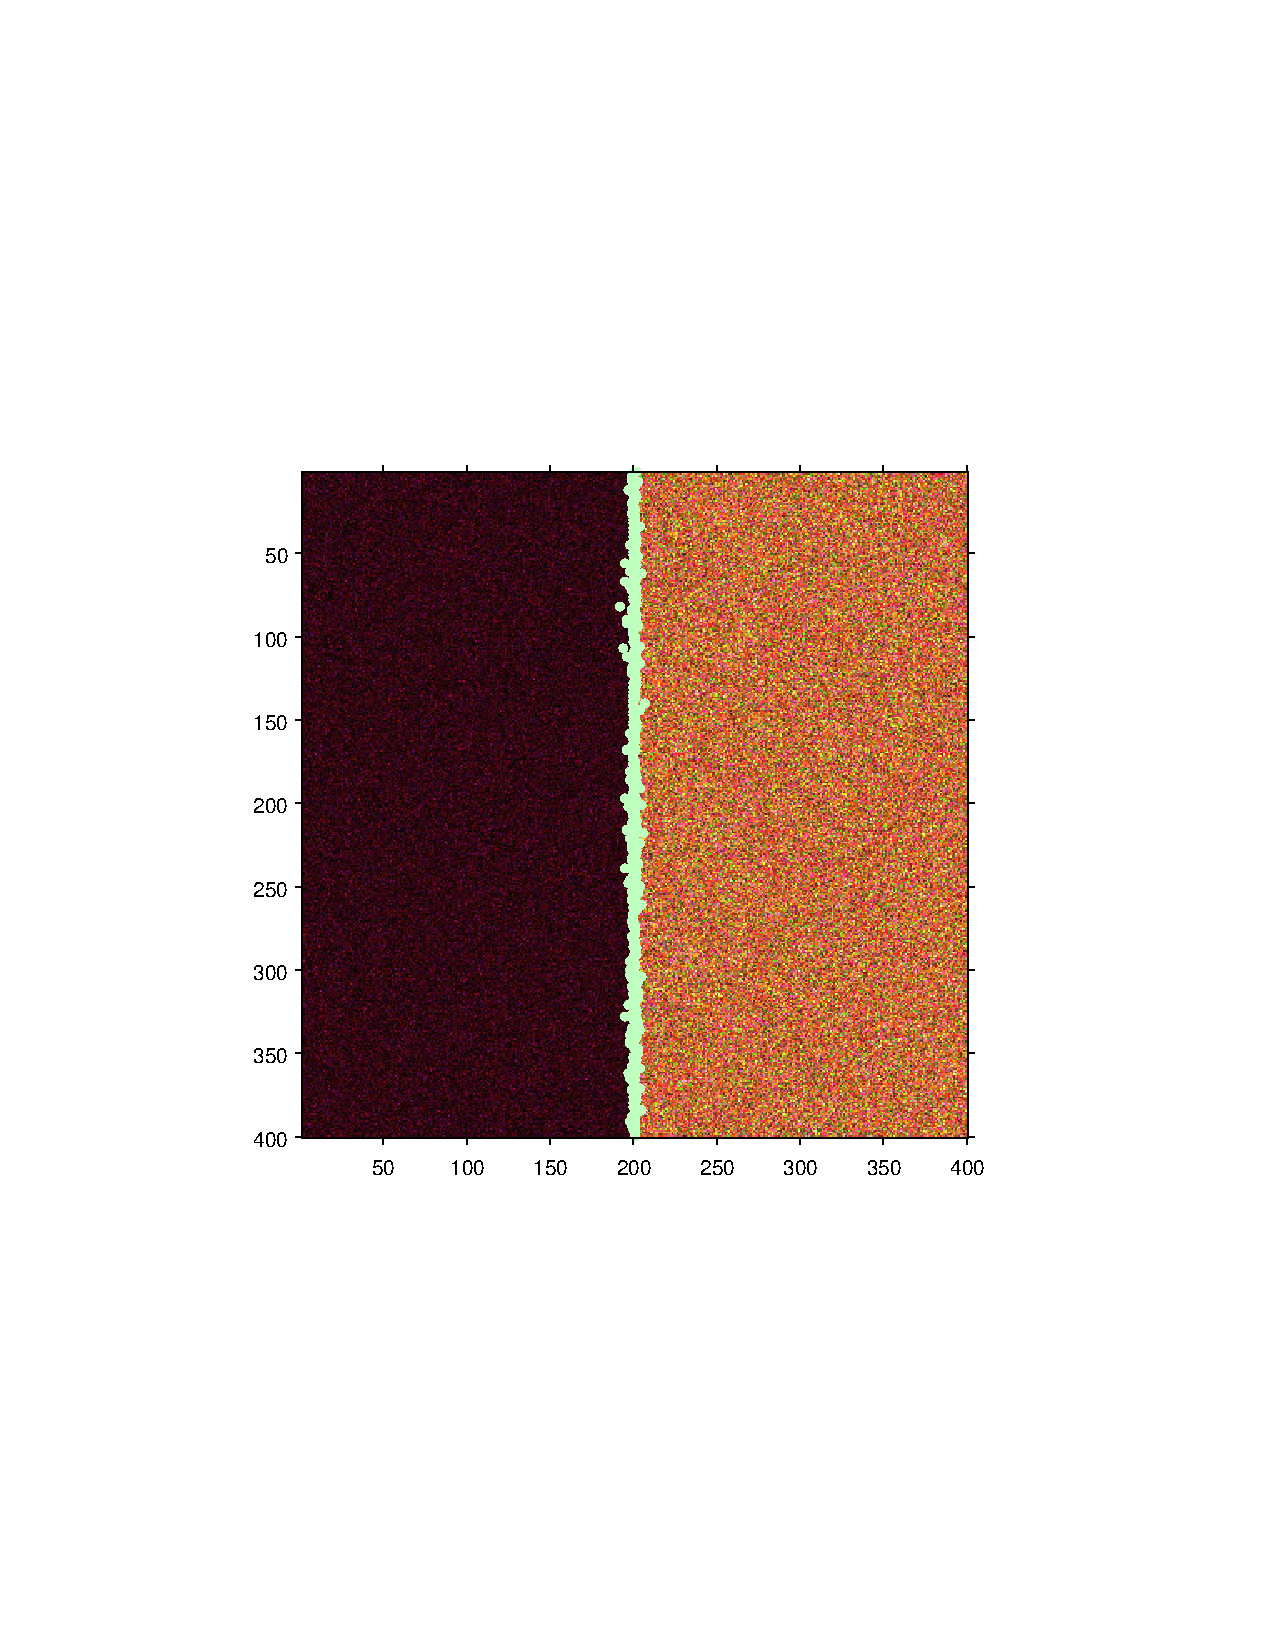
\includegraphics[width=.7\linewidth]{im_sim_gamf_span_media_mu_14_pixel}%
	\caption{Evidências de bordas para o span (media estimada)}
\label{fig:evidencias_span_gamf}
\end{figure}
    
    
    
%The error is measured simulating $400$ independent images and finding $\widehat\jmath$ in a line fixed.
%By construction, the vertical line $200$ is considered as the real edge in each replication, so the error for this replication is the absolute value of the difference between this point and the estimated value, and it is computed by $E(r) = |200 - \widehat{\jmath}(r)|$, $1\leq r \leq 400$.

%Relative frequencies to estimate the probability of having an error smaller than a number of pixels is used. 
%Denoting $H(k)$ the number of replications for which the error is less than $k$ pixels, an estimate of this probability is $f(k)=\frac{H(k)}{400}$. 
%In the tests performed in this section, $k$ varies between $1$ and $10$. 
%The algorithm is described in Ref.~\cite{fbgm}.
%Fig.~\ref{probability_edge_detc} shows these probabilities as computed in each channel $I_\text{hh}$, $I_\text{hv}$ and $I_{vv}$ of the image.

%




%A figura \eqref{fig:pdf_mag_prod} mostra a função densidade magnitude do produto com a variação das visadas $L=2,3,4$, e $8$, 
%\begin{figure}[hbt]
%\centering
%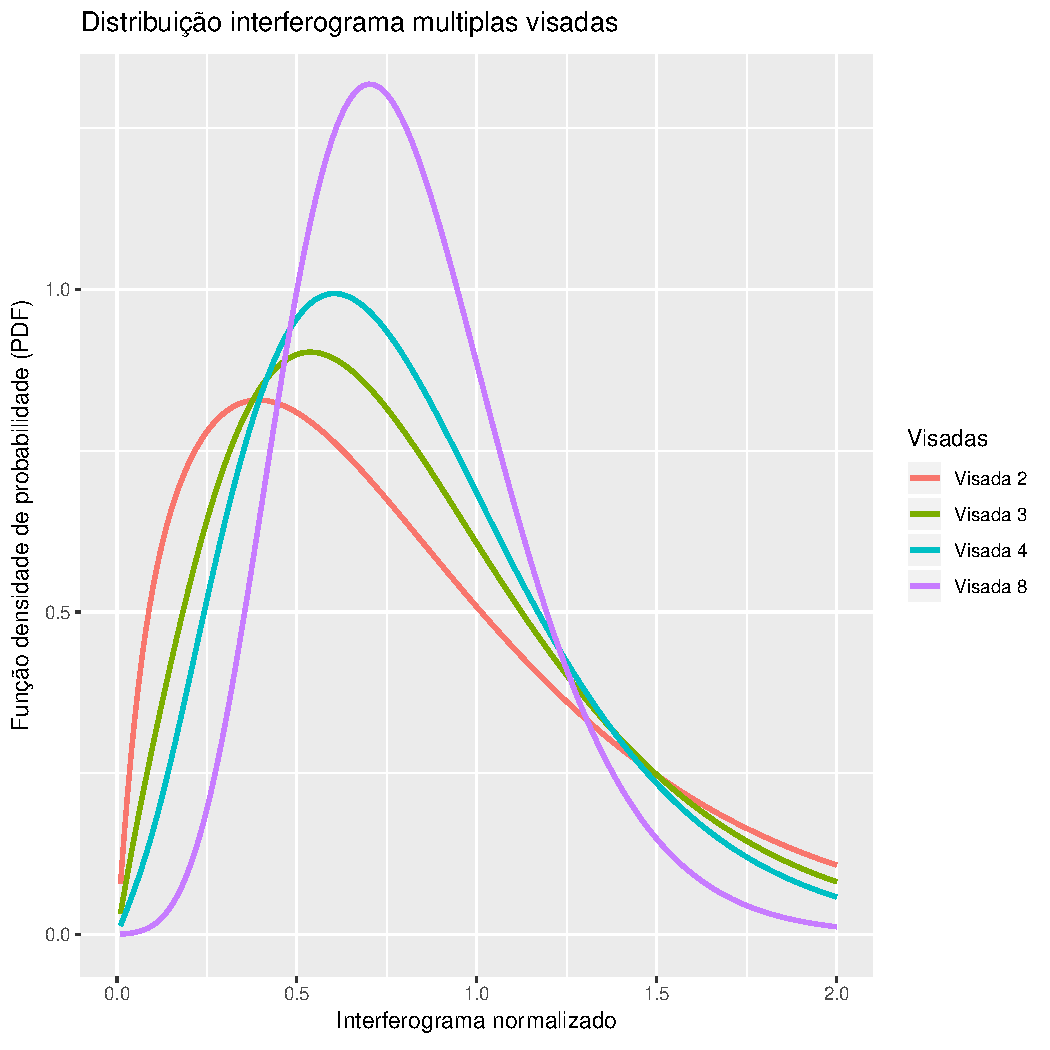
\includegraphics[width=4.0in]{dist_interferograma_multi_visadas.pdf}
%	\caption{Distribuição magnitude do produto múltiplas visadas.}
%\label{fig:pdf_mag_prod}
%\end{figure}


%
%As figuras \eqref{fig:prod_mag_l_50_r_35} até \eqref{fig:prod_mag_l_350_r_35} mostram a função de log-verossimilhança da pdf magnitude de produtos \eqref{eq:eq_log_vero_mag_prod_red} aplicada para a amostra de duas folhas simulada. No processo fixamos arbitrariamente a linha 35 da amostra e variamos o número de pixel entre 50, 150, 250 e 250. Desta maneira construímos duas funções $\ell{j}$, uma para cada lado da amostra.
% \begin{figure*}[hbt]
%	\centering
%     \subfloat[Pixel variando de 1 até 50 na linha 35.  \label{fig:prod_mag_l_rho_1_50}]{%
%       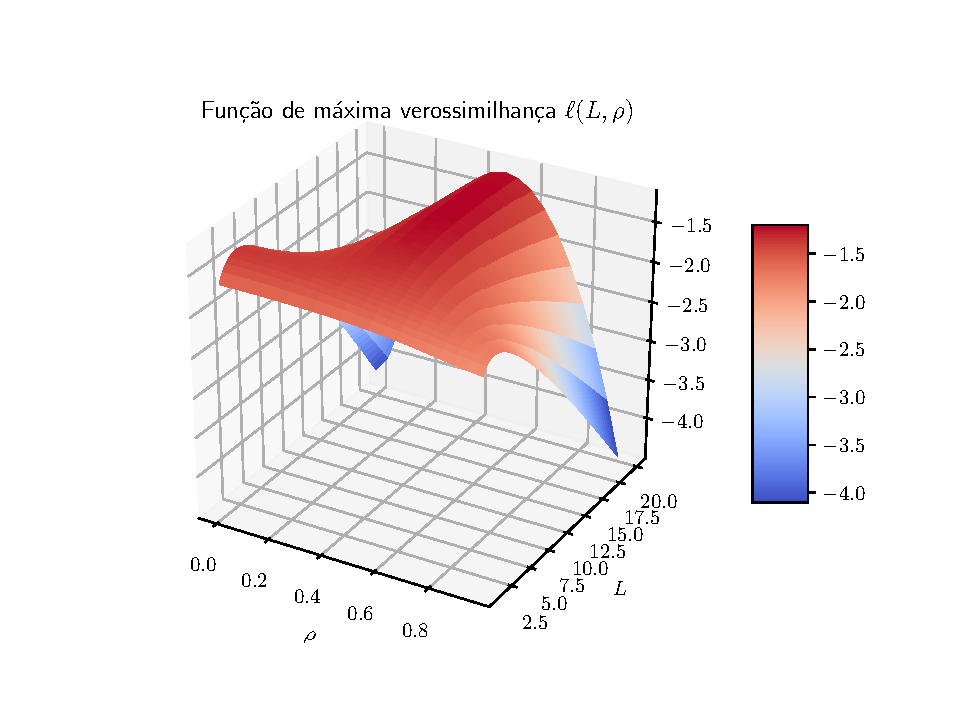
\includegraphics[width=0.50\linewidth]{fig_pdf_mag_prod_r_35_1_to_50}
%     }
%     \subfloat[Pixel variando de 51 até 400 na linha 35. \label{fig:prod_mag_l_rho_51_400}]{%
%       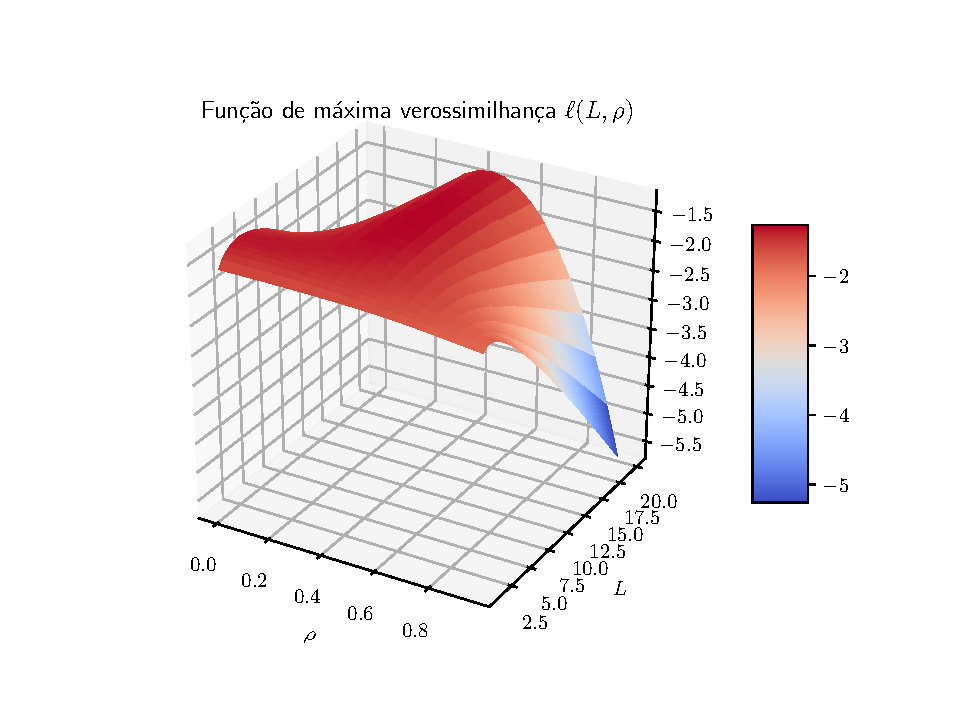
\includegraphics[width=0.50\linewidth]{fig_pdf_mag_prod_r_35_51_to_400}
%     }
%     \caption{Funções de máxima verossimilhança produto de magnitude com pixel fixo 50.}
%     \label{fig:prod_mag_l_50_r_35} 
%   \end{figure*}
%   
%   \begin{figure*}[hbt]
%	\centering
%     \subfloat[Pixel variando de 1 até 150 na linha 35.  \label{fig:prod_mag_l_rho_1_150}]{%
%       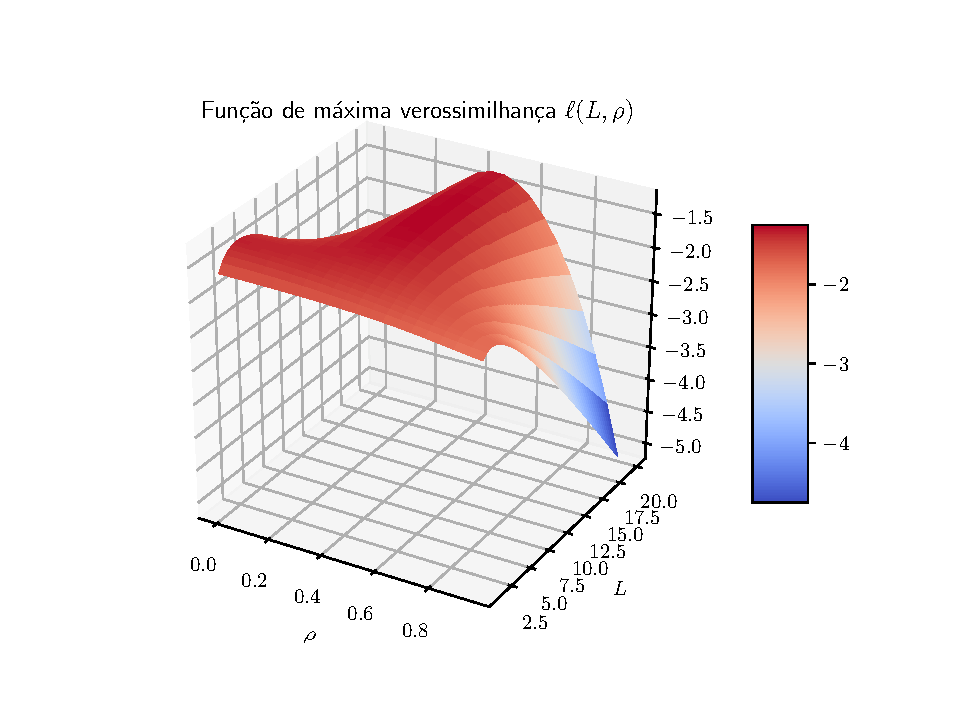
\includegraphics[width=0.50\linewidth]{fig_pdf_mag_prod_r_35_1_to_150}
%     }
%     \subfloat[Pixel variando de 151 até 400 na linha 35. \label{fig:prod_mag_l_rho_151_400}]{%
%       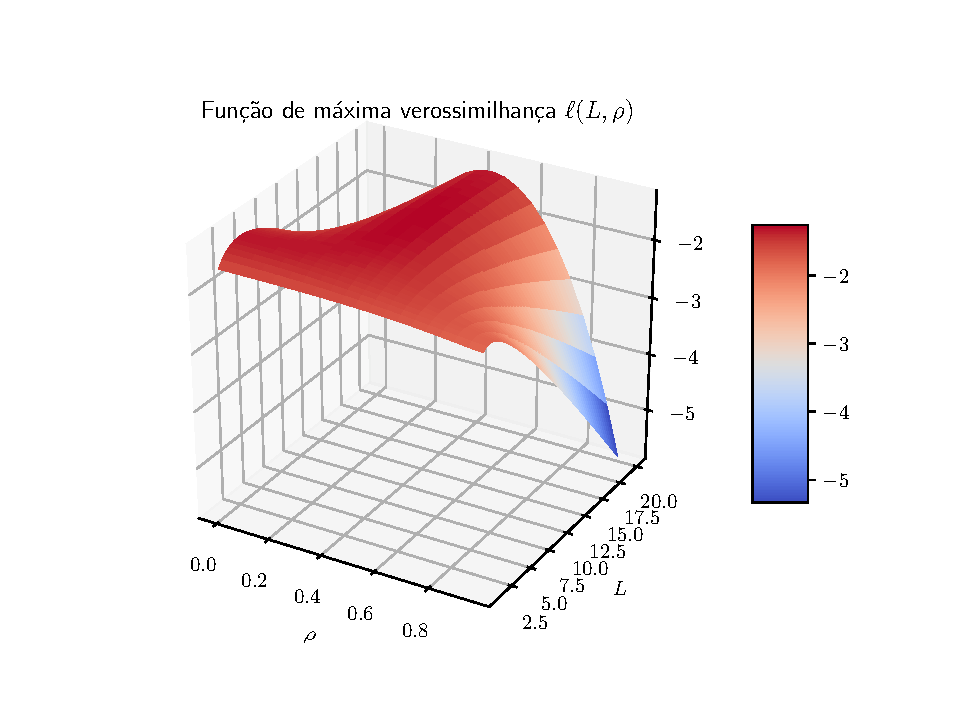
\includegraphics[width=0.50\linewidth]{fig_pdf_mag_prod_r_35_151_to_400}
%     }
%     \caption{Funções de máxima verossimilhança produto de magnitude com pixel fixo 150.}
%     \label{fig:prod_mag_l_150_r_35} 
%   \end{figure*}
%
%\begin{figure*}[hbt]
%	\centering
%     \subfloat[Pixel variando de 1 até 250 na linha 35.  \label{fig:prod_mag_l_rho_1_250}]{%
%       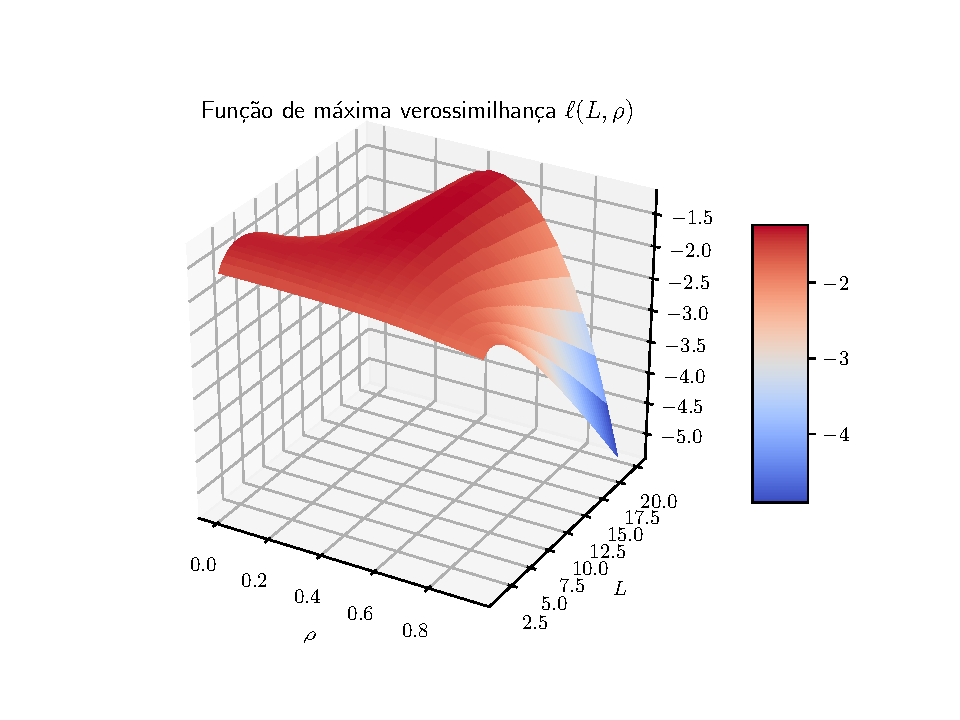
\includegraphics[width=0.50\linewidth]{fig_pdf_mag_prod_r_35_1_to_250}
%     }
%     \subfloat[Pixel variando de 251 até 400 na linha 35. \label{fig:prod_mag_l_rho_251_400}]{%
%       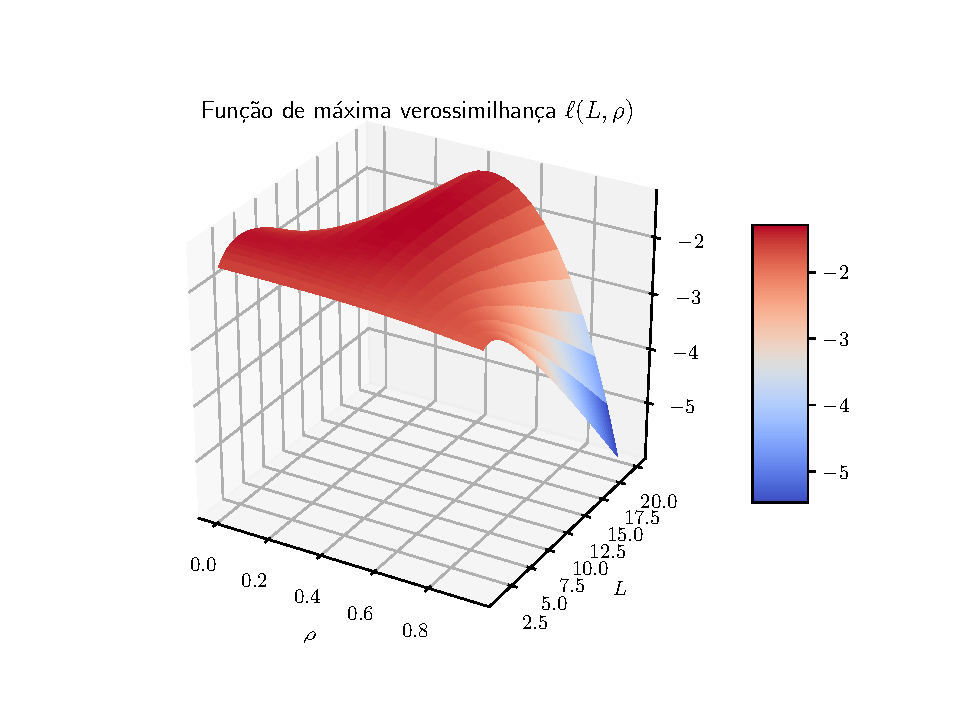
\includegraphics[width=0.50\linewidth]{fig_pdf_mag_prod_r_35_251_to_400}
%     }
%     \caption{Funções de máxima verossimilhança produto de magnitude com pixel fixo 250.}
%     \label{fig:prod_mag_l_250_r_35} 
%   \end{figure*}
%   \begin{figure*}[hbt]
%	\centering
%     \subfloat[Pixel variando de 1 até 350 na linha 35.  \label{fig:prod_mag_l_rho_1_350}]{%
%       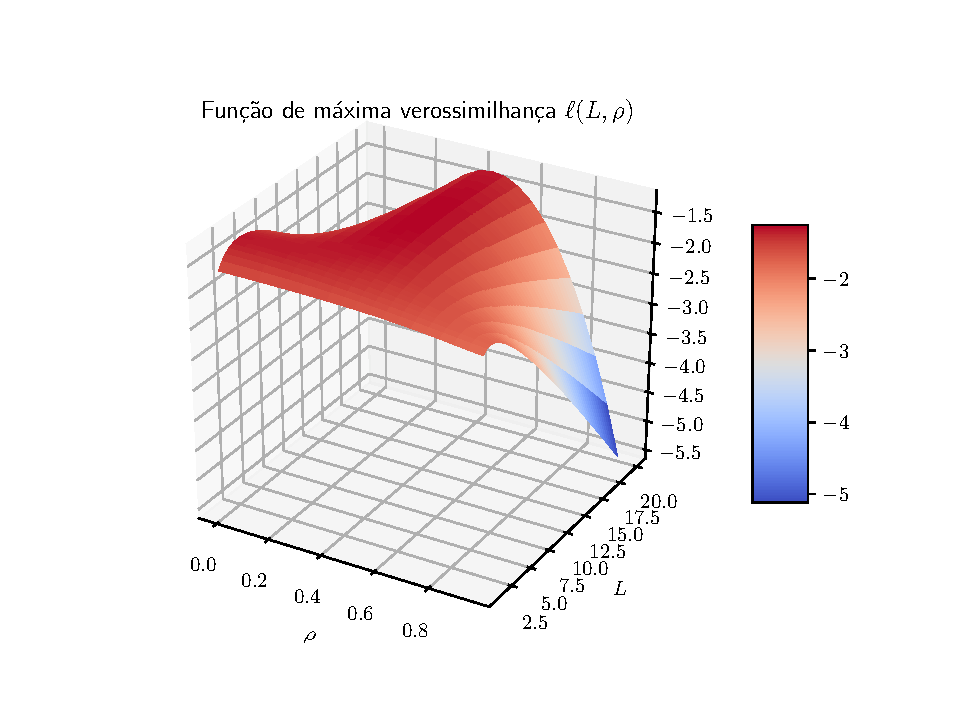
\includegraphics[width=0.50\linewidth]{fig_pdf_mag_prod_r_35_1_to_350}
%     }
%     \subfloat[Pixel variando de 351 até 400 na linha 35. \label{fig:prod_mag_l_rho_351_400}]{%
%       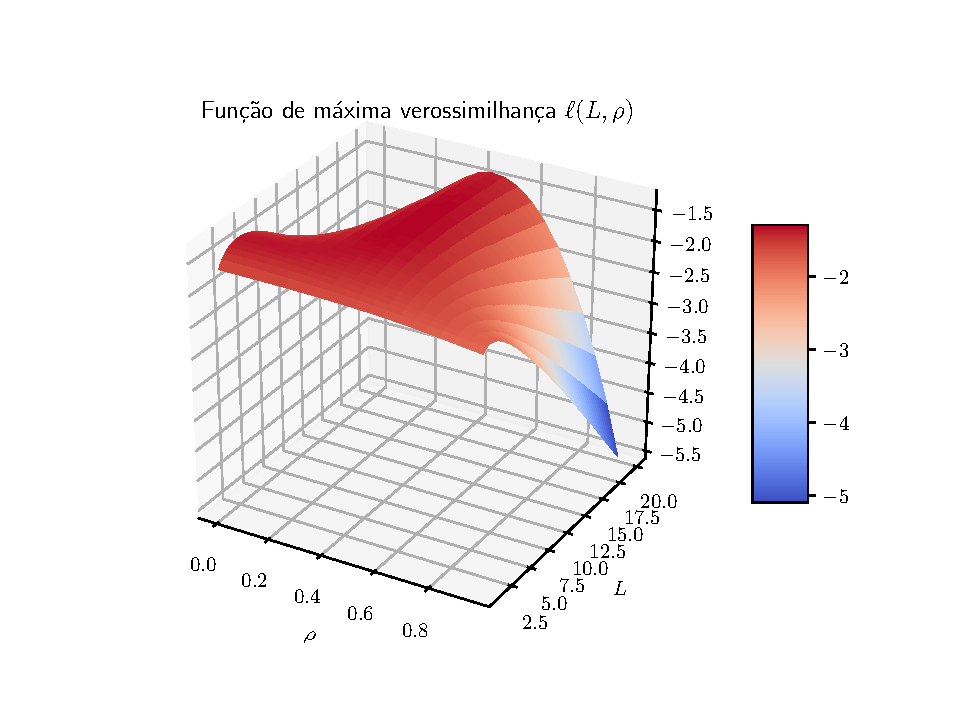
\includegraphics[width=0.50\linewidth]{fig_pdf_mag_prod_r_35_351_to_400}
%     }
%     \caption{Funções de máxima verossimilhança produto de magnitude com pixel fixo 350.}
%     \label{fig:prod_mag_l_350_r_35} 
%   \end{figure*}

%As figuras \eqref{fig:prod_mag_l_25_r_50_hh}, \eqref{fig:prod_mag_l_25_r_50_hv} e \eqref{fig:prod_mag_l_25_r_50_vv} mostram a função de log-verossimilhança da pdf magnitude de produtos \eqref{eq:eq_log_vero_mag_prod_red} aplicada na ROI da imagem de flevoland. No processo fixamos arbitrariamente a radial 50 da amostra e fixamos o número de pixel 50. Desta maneira construímos duas funções $\ell{j}$ em cada lado da radial. Os gráficos das funções foram gerados para os canais de intensidades.

%Na figura \eqref{fig:prod_mag_l_rho_1_25_hh} podemos identificar o problema da função ser plana dificultando muito o processo de encontrar o ponto de máximo gerando oscilação na função $\ell(j)$. Na \eqref{fig:prod_mag_l_rho_26_120_hh} ocorre o problema das funções de bessel serem infinitas quando seu argumento assume valores grande, também dificultando o cálculo do valor máximo.  

%\begin{figure*}[hbt]
%	\centering
%     \subfloat[Pixel variando de 1 até 25 na radial 50 no canal (hh).  \label{fig:prod_mag_l_rho_1_25_hh}]{%
%       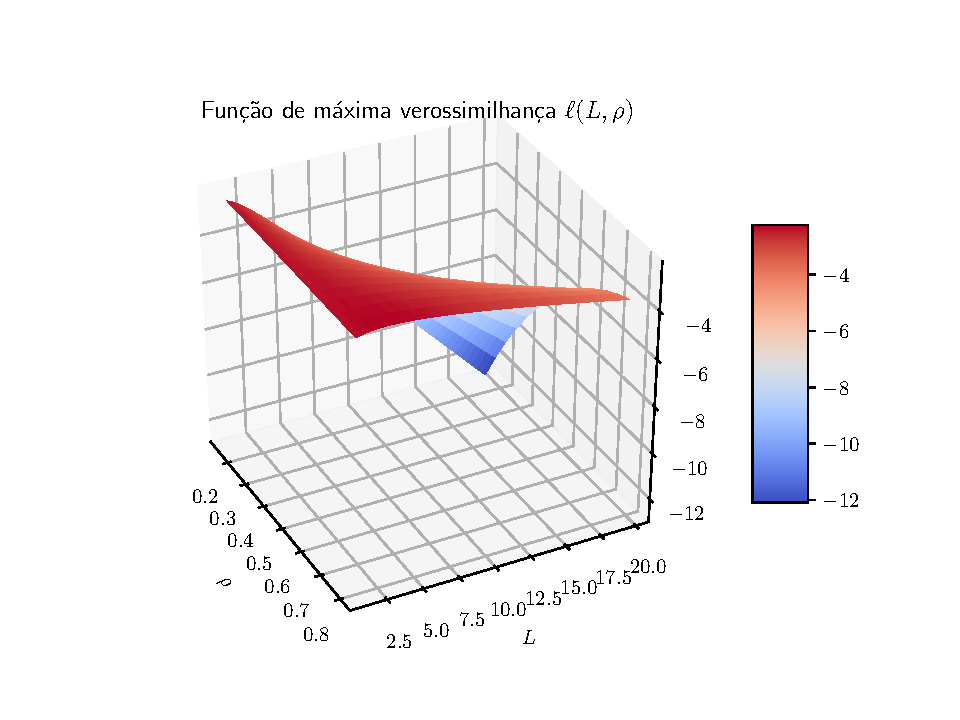
\includegraphics[width=0.50\linewidth]{fig_pdf_mag_prod_r_50_1_to_25_flev}
%     }
%     \subfloat[Pixel variando de 26 até 120 na radial 50 no canal (hh). \label{fig:prod_mag_l_rho_26_120_hh}]{%
%       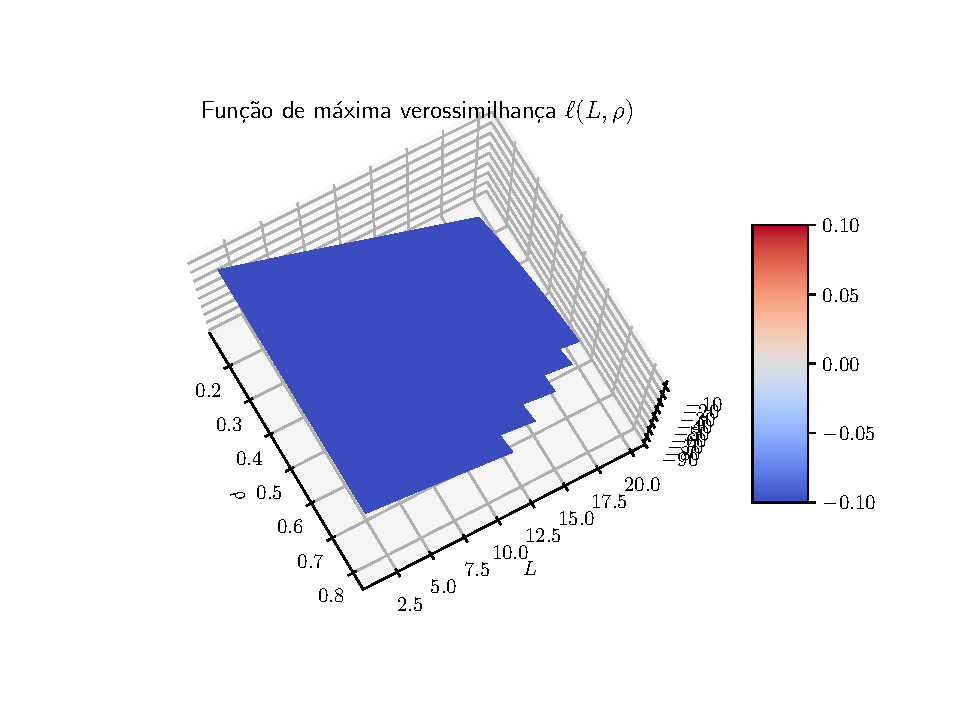
\includegraphics[width=0.50\linewidth]{fig_pdf_mag_prod_r_50_26_to_120_flev}
%     }
%     \caption{Funções de máxima verossimilhança produto de magnitude com pixel fixo 25 no canal (hh).}
%     \label{fig:prod_mag_l_25_r_50_hh} 
%   \end{figure*}
   
%Nas figuras de \eqref{fig:prod_mag_l_25_r_50_hv} destacamos o problema da função ser plana. Assim como em no gráfico da função \eqref{fig:prod_mag_l_rho_1_25_hh} 
%\begin{figure*}[hbt]
%	\centering
%     \subfloat[Pixel variando de 1 até 25 na radial 50 no canal (hv).  \label{fig:prod_mag_l_rho_1_25_hv}]{%
%       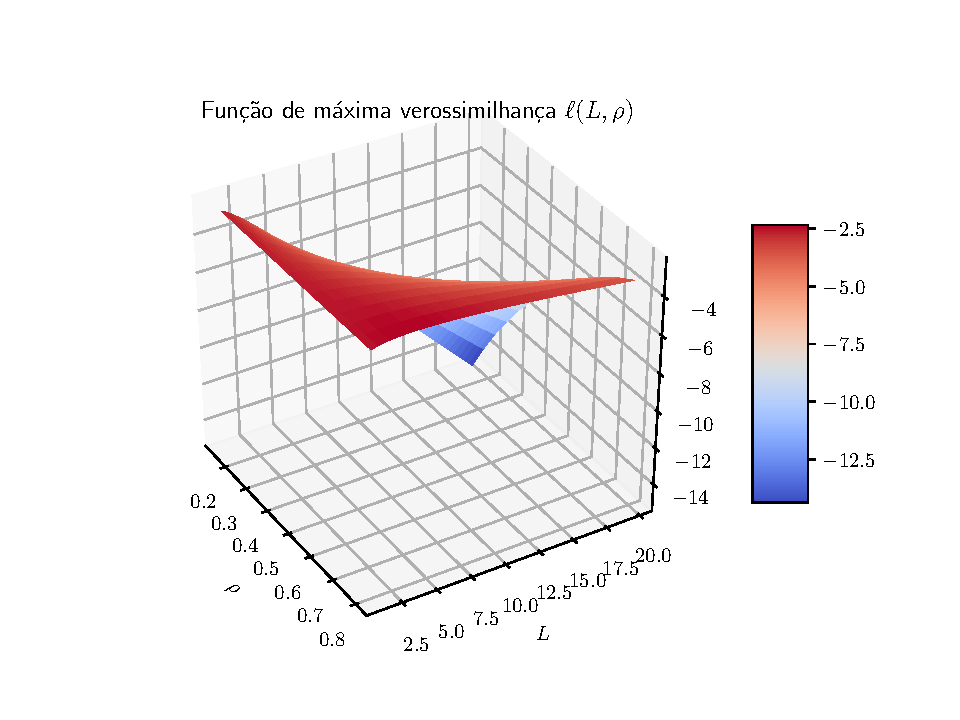
\includegraphics[width=0.50\linewidth]{fig_pdf_mag_prod_r_50_1_to_25_flev_hv}
%     }
%     \subfloat[Pixel variando de 26 até 120 na radial 50 no canal (hv). \label{fig:prod_mag_l_rho_26_120_hv}]{%
%       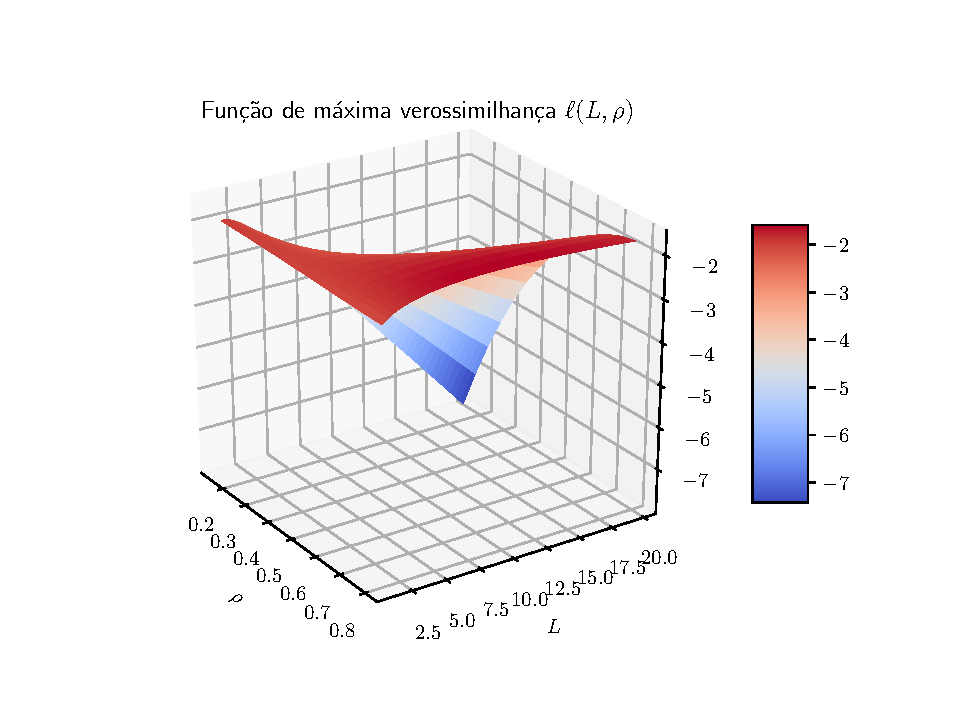
\includegraphics[width=0.50\linewidth]{fig_pdf_mag_prod_r_50_26_to_120_flev_hv}
%     }
%     \caption{Funções de máxima verossimilhança produto de magnitude com pixel fixo 25 no canal (hv).}
%     \label{fig:prod_mag_l_25_r_50_hv} 
%   \end{figure*}
%
%Nas figuras de \eqref{fig:prod_mag_l_25_r_50_vv} destacamos o problema da função ser plana. Assim como em no gráfico da função \eqref{fig:prod_mag_l_rho_1_25_hh} 
%
%\begin{figure*}[hbt]
%	\centering
%     \subfloat[Pixel variando de 1 até 25 na radial 50 no canal (vv).  \label{fig:prod_mag_l_rho_1_25_vv}]{%
%       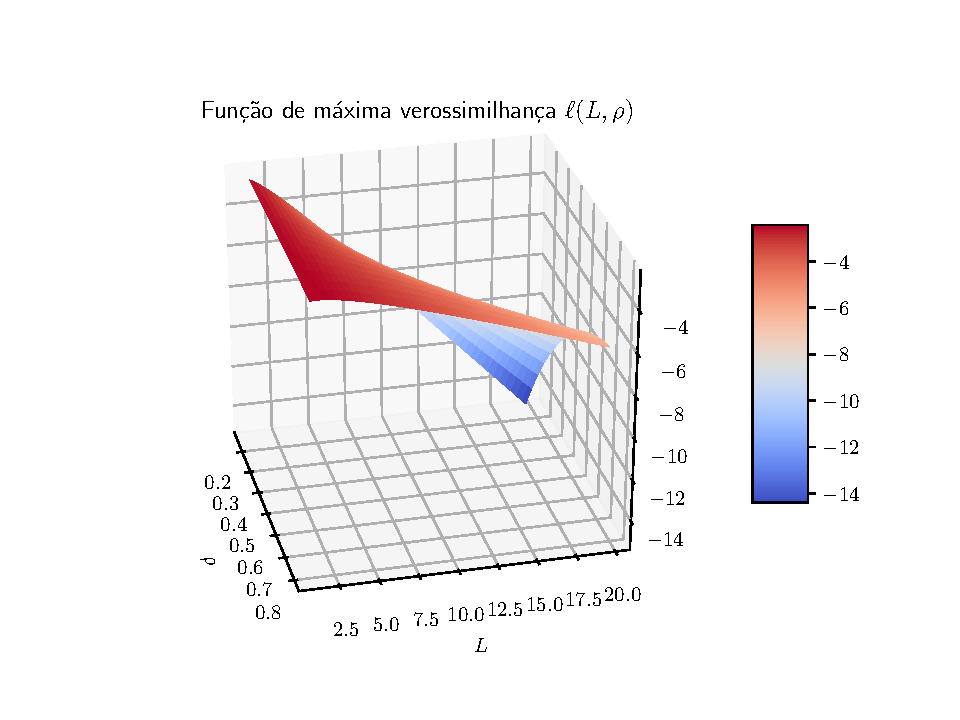
\includegraphics[width=0.50\linewidth]{fig_pdf_mag_prod_r_50_1_to_25_flev_vv}
%     }
%     \subfloat[Pixel variando de 26 até 120 na radial 50 no canal (vv). \label{fig:prod_mag_l_rho_26_120_vv}]{%
%       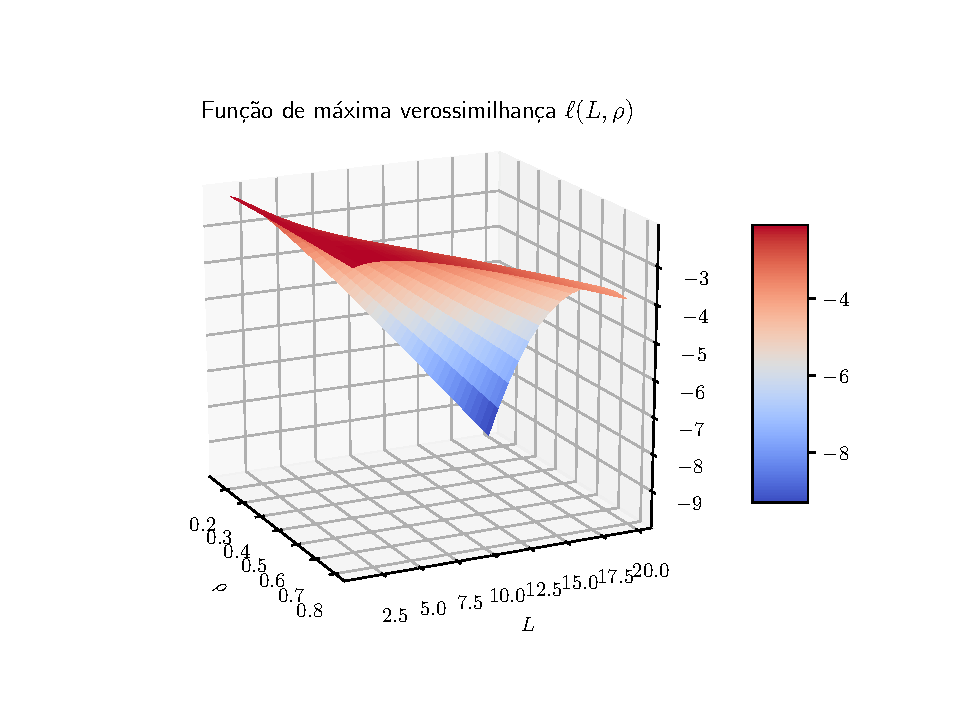
\includegraphics[width=0.50\linewidth]{fig_pdf_mag_prod_r_50_26_to_120_flev_vv}
%     }
%     \caption{Funções de máxima verossimilhança produto de magnitude com pixel fixo 25 no canal (vv).}
%     \label{fig:prod_mag_l_25_r_50_vv} 
%   \end{figure*}


%\subsubsection{Aplicação na imagem simulada com duas amostras}


%As figuras \eqref{fig:razao_tau_rho_1_50} até \eqref{fig:razao_tau_rho_51_400} mostram a função de log-verossimilhança da pdf razão de intensidades \eqref{eq:pdf_razao_intensidades_tau_w} aplicada na imagem de duas amostras simulada. No processo fixamos arbitrariamente a linha 80 da amostra e variamos o número de pixel entre 50, 150, 250 e 250. Desta maneira construímos duas funções $\ell{j}$, uma para cada lado da amostra. Nessas figuras fixamos o L = 4 e os canais (hh) e (vv).
% \begin{figure*}[hbt]
%	\centering
%     \subfloat[Pixel variando de 1 até 50 na linha 80.  \label{fig:razao_tau_rho_1_50}]{%
%       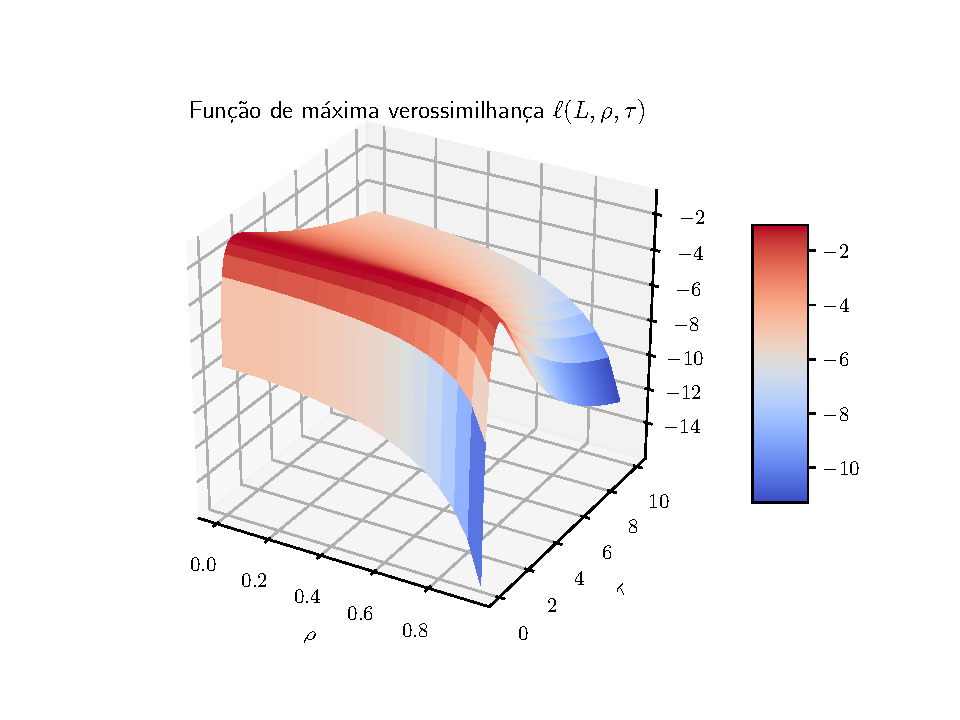
\includegraphics[width=0.50\linewidth]{fig_pdf_razao_r_80_1_to_50}
%     }
%     \subfloat[Pixel variando de 51 até 400 na linha 80. \label{fig:razao_tau_rho_51_400}]{%
%       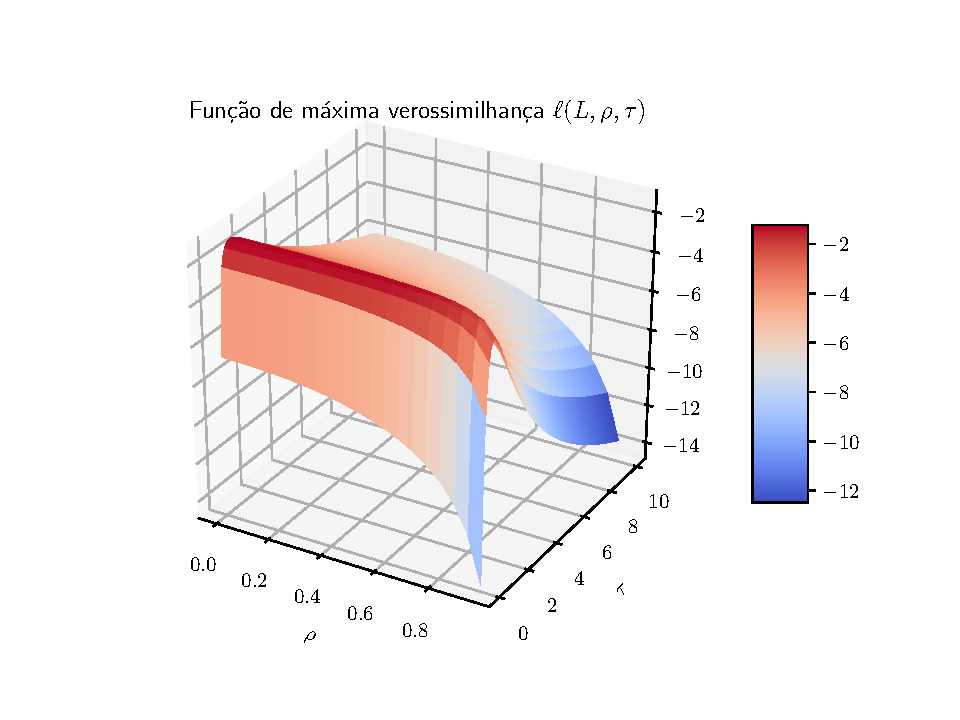
\includegraphics[width=0.50\linewidth]{fig_pdf_razao_r_80_50_to_400}
%     }
%     \caption{Funções de máxima verossimilhança razão de intensidades com pixel fixo 50.}
%     \label{fig:razao_l_50_r_80} 
%   \end{figure*}
%\begin{figure*}[hbt]
%	\centering
%     \subfloat[Pixel variando de 1 até 150 na linha 80.  \label{fig:razao_tau_rho_1_150}]{%
%       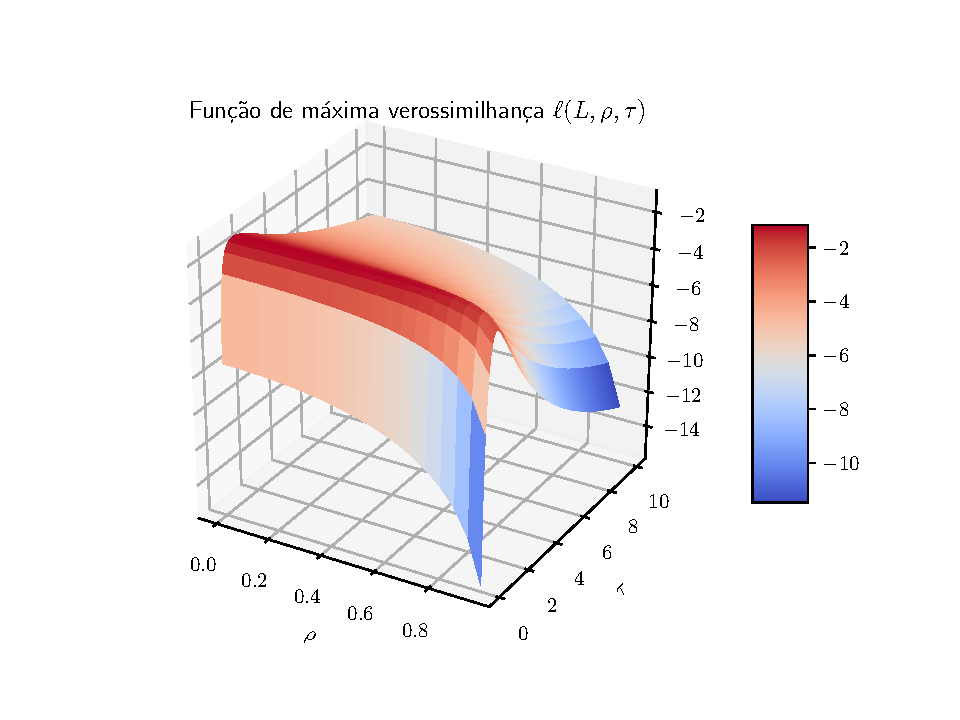
\includegraphics[width=0.50\linewidth]{fig_pdf_razao_r_80_1_to_150}
%     }
%     \subfloat[Pixel variando de 151 até 400 na linha 80. \label{fig:razao_tau_rho_151_400}]{%
%       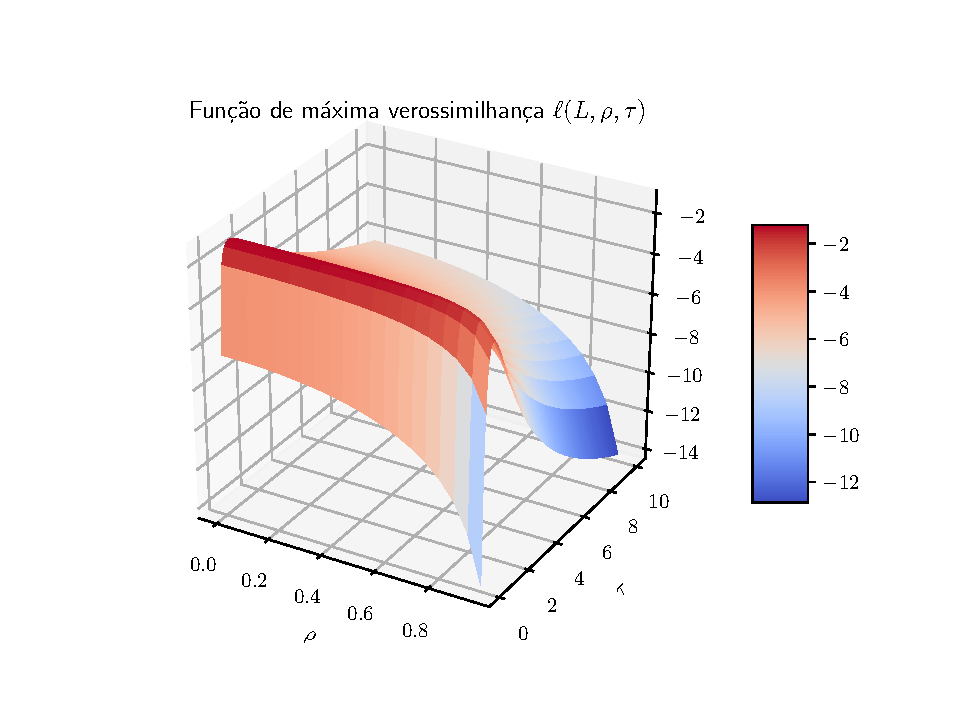
\includegraphics[width=0.50\linewidth]{fig_pdf_razao_r_80_150_to_400}
%     }
%     \caption{Funções de máxima verossimilhança razão de intensidades com pixel fixo 150.}
%     \label{fig:razao_l_150_r_80} 
%   \end{figure*}   
%   
%   \begin{figure*}[hbt]
%	\centering
%     \subfloat[Pixel variando de 1 até 250 na linha 80.  \label{fig:razao_tau_rho_1_250}]{%
%       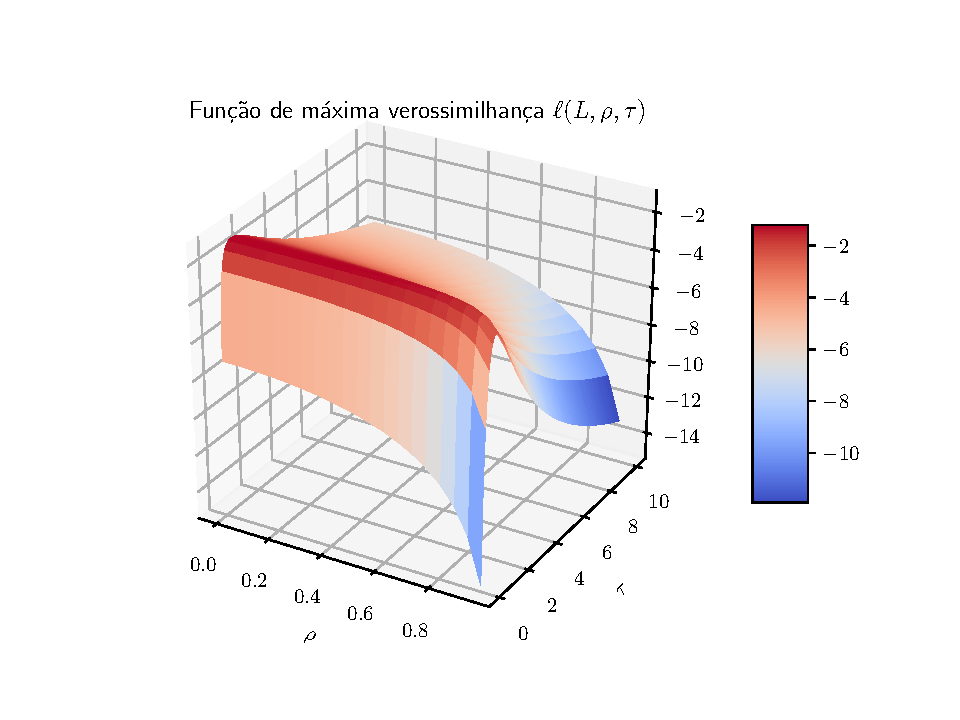
\includegraphics[width=0.50\linewidth]{fig_pdf_razao_r_80_1_to_250}
%     }
%     \subfloat[Pixel variando de 251 até 400 na linha 80. \label{fig:razao_tau_rho_251_400}]{%
%       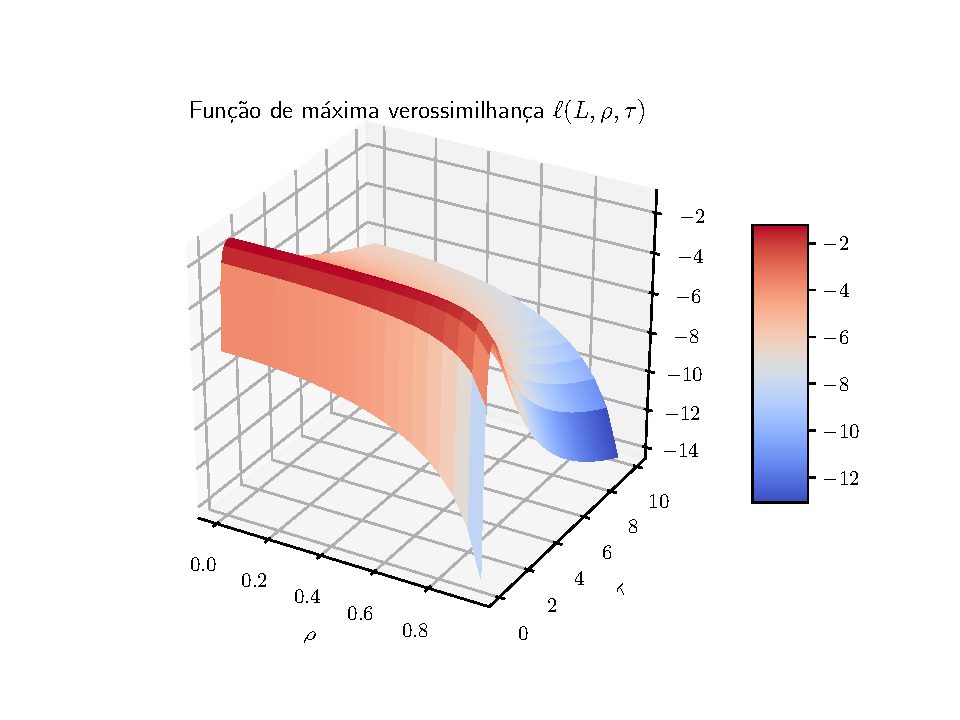
\includegraphics[width=0.50\linewidth]{fig_pdf_razao_r_80_250_to_400}
%     }
%     \caption{Funções de máxima verossimilhança razão de intensidades com pixel fixo 250.}
%     \label{fig:razao_l_250_r_80} 
%   \end{figure*}   
%   
%   \begin{figure*}[hbt]
%	\centering
%     \subfloat[Pixel variando de 1 até 350 na linha 80.  \label{fig:razao_tau_rho_1_350}]{%
%       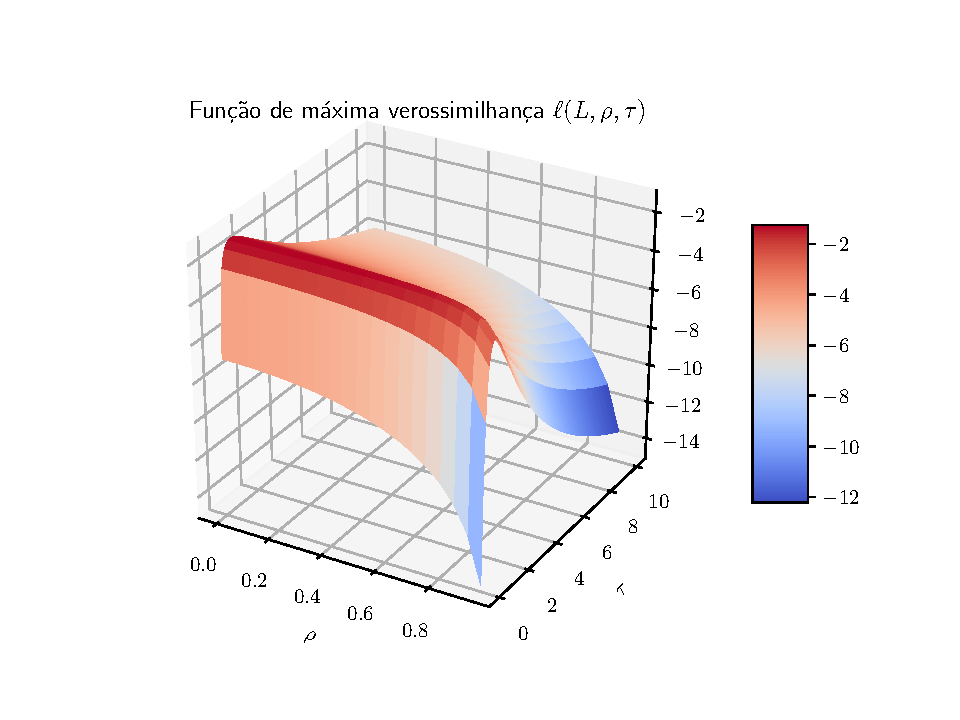
\includegraphics[width=0.50\linewidth]{fig_pdf_razao_r_80_1_to_350}
%     }
%     \subfloat[Pixel variando de 351 até 400 na linha 80. \label{fig:razao_tau_rho_351_400}]{%
%       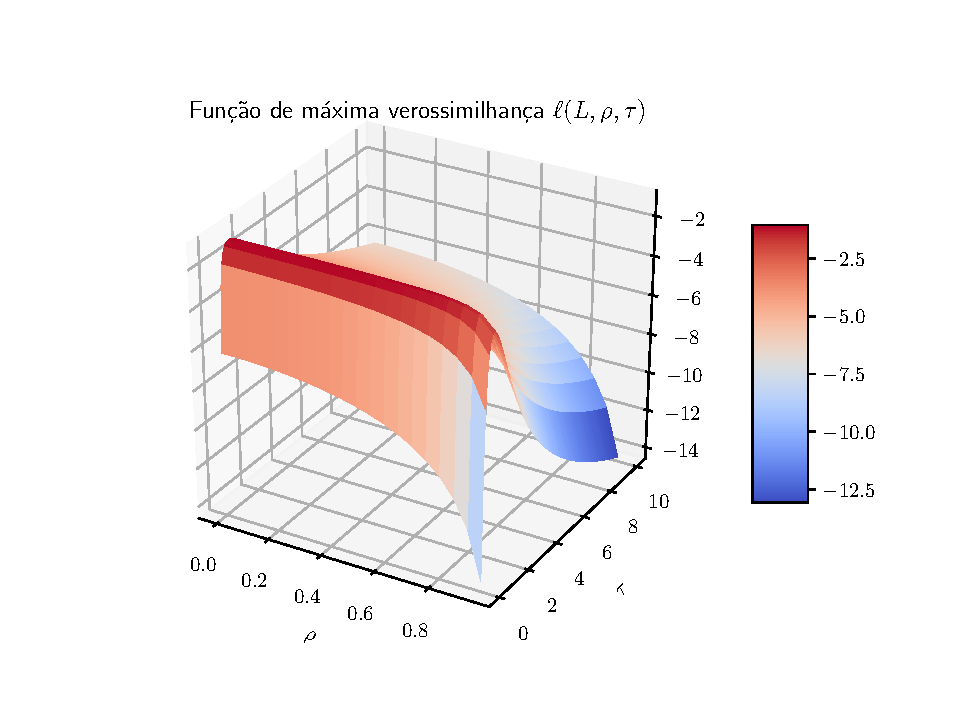
\includegraphics[width=0.50\linewidth]{fig_pdf_razao_r_80_350_to_400}
%     }
%     \caption{Funções de máxima verossimilhança razão de intensidades com pixel fixo 350.}
%     \label{fig:razao_l_250_r_80} 
%   \end{figure*}   
   

%O método da máxima verossimilhança \eqref{eq:TotalLogLikelihood} foi aplicado na imagem simulada com duas amostras, e as evidências de bordas estão mostradas na figura. \textcolor{red}{Base de dados gamf}
% \begin{figure*}[hbt]
%	\centering
%     \subfloat[Evidências no canal $\text{hh}$ \label{evidencias_hh_hv_vv_gamf:a}]{%
%       \includegraphics[width=0.5\linewidth]{im_sim_gamf_hh_hv_param_tau_rho_14_pixel}
%     }
%     \subfloat[xxxxxxxxxxxxxxxxxx $\text{hv}$ \label{evidencias_hh_hv_vv_gamf:b}]{%
%       \includegraphics[width=0.5\linewidth]{im_sim_gamf_hh_vv_param_tau_rho_14_pixel}
%     }      
%   %  \subfloat[Evidências no canal $\text{vv}$ \label{evidencias_hh_hv_vv_gamf:c}]{%
%    %   \includegraphics[width=0.5\linewidth]{im_sim_gamf_hh_evid_param_L_mu_14_pixel}
%    % }
%    \caption{Evidências de bordas para os três canais de intensidade}
%     \label{evidencias_hh_hv_vv_gamf} 
%   \end{figure*}
%   
%   \begin{figure*}[hbt]
%	\centering
%     \subfloat[Evidências no canal $\text{vv}$ \label{evidencias_hh_hv_vv_gamf:c}]{%
%       \includegraphics[width=0.5\linewidth]{im_sim_gamf_hv_vv_param_tau_rho_14_pixel}
%     }
%    \caption{Evidências de bordas para os três canais de intensidade}
%     \label{evidencias_hh_hv_vv_gamf} 
%   \end{figure*}   
   

%\section{Resultados numéricos para o método MLE aplicado em cada distribuíção}

%Usamos uma imagem AIRSAR PolSAR de Flevoland, banda L, de $750\times 1024$ pixels para os testes.  Fig.~\ref{flevoland_radial_4look} mostra o ROI, com as linhas radiais onde as bordas são detectadas. Fig.~\ref{flevoland_flevoland} mostra a referência do solo em vermelho.  
%  \begin{figure}[hbt]
%   \centering
%     \subfloat[Imagem, Região de Interesse (ROI), and radiais. \label{flevoland_radial_4look}]{%
%%       \includegraphics[viewport= 0 50 500 550, clip=true, width=0.23\textwidth]{flevoland_radial_4_look_black_crop}}      
%       \includegraphics[width=0.53\textwidth]{flevoland_radial_4_look_black_crop}}
%     \subfloat[Ground reference\label{gt_flevoland}]{%
%       \includegraphics[width=0.5\textwidth]{gt_flevoland_crop}
%     }
%    \caption{Decomposição de Pauli para a imagem de Flevoland, região de interesse, e referência \textit{ground}}
%    \label{roi_gt}
%\end{figure}

%\subsection{Método da verossimilhança aplicado na pdf univariada $\Gamma$.}
%Resolvendo o problema,
%$$
%\widehat{\jmath}= \arg\max\limits_{j\in [\min_s,N-\min_s]}\ell(j;\widehat{\rho}_I, \widehat{L}_I,\widehat{\rho}_E, \widehat{L}_E),
%$$

%Figs.~\ref{evidencias_hh_hv_vv}\subref{evidencias_hh_hv_vv:a},~\ref{evidencias_hh_hv_vv}\subref{evidencias_hh_hv_vv:b}, e~\ref{evidencias_hh_hv_vv:a}\subref{evidencias_hh_hv_vv:c}, mostram, respectivamente, as evidências de borda nos canais $\text{hh}$, $\text{hv}$ e $\text{vv}$ como obtidos pela MLE.

%Vale notar que a GenSA identificou com precisão o valor máximo de $\eqref{eq:TotalLogLikelihood}$, mesmo na presença de múltiplos máximos locais. 
%Uma avaliação visual leva à conclusão de que os melhores resultados são fornecidos por $\text{hv}$, embora com alguns pontos longe da borda real.

% \begin{figure*}[hbt]
%	\centering
%     \subfloat[Evidências no canal $\text{hh}$ \label{evidencias_hh_hv_vv:a}]{%
%       \includegraphics[width=0.32\linewidth]{flevoland_hh_evid_param_L_mu_14_pixel_crop}
%     }
%     \subfloat[Evidências no canal $\text{hv}$ \label{evidencias_hh_hv_vv:b}]{%
%       \includegraphics[width=0.32\linewidth]{flevoland_hv_evid_param_L_mu_14_pixel_crop}
%     }
%     \subfloat[Evidências no canal $\text{vv}$ \label{evidencias_hh_hv_vv:c}]{%
%       \includegraphics[width=0.32\linewidth]{flevoland_vv_evid_param_L_mu_14_pixel_crop}
%     }
%     \caption{Evidências de bordas para os três canais de intensidade}
%     \label{evidencias_hh_hv_vv} 
%   \end{figure*}

%\subsection{Método da verossimilhança aplicado na pdf magnitude do produto.}


% \begin{figure*}[hbt]
%	\centering
%     \subfloat[Evidências no canal $\text{hh}$ \label{evidencias_hh_hv_vv:a}]{%
%       \includegraphics[width=0.32\linewidth]{}
%     }
%     \subfloat[Evidências no canal $\text{hv}$ \label{evidencias_hh_hv_vv:b}]{%
%       \includegraphics[width=0.32\linewidth]{flevoland_hv_evid_param_L_mu_14_pixel_crop}
%     }
%     \subfloat[Evidências no canal $\text{vv}$ \label{evidencias_hh_hv_vv:c}]{%
%       \includegraphics[width=0.32\linewidth]{flevoland_vv_evid_param_L_mu_14_pixel_crop}
%     }
%     \caption{Evidências de bordas para os três canais de intensidade}
%     \label{evidencias_hh_hv_vv} 
%   \end{figure*}


%\begin{figure}[hbt]
%\minipage{0.5\textwidth}
%  \includegraphics[width=\linewidth]{funv_max_ver_j_10_flev_razao.pdf}
%  	\caption{$\sigma= 12.3426$.}\label{cap_acf_fig04}
%\endminipage\hfill
%\minipage{0.5\textwidth}
%  \includegraphics[width=\linewidth]{funv_max_ver_j_20_flev_razao.pdf}
%		\caption{$\sigma=2.1029 $.}\label{cap_acf_fig05}
%\endminipage\hfill
%\centering
%\minipage{0.5\textwidth}
%  \includegraphics[width=\linewidth]{funv_max_ver_j_30_flev_razao.pdf}
%  	\caption{$\sigma=1.4999 $.}\label{cap_acf_fig04}
%\endminipage\hfill
%\minipage{0.5\textwidth}
%  \includegraphics[width=\linewidth]{funv_max_ver_j_40_flev_razao.pdf}
%		\caption{$\sigma=12.6414 $.}\label{cap_acf_fig05}
%\endminipage\hfill
%\end{figure}
%\begin{figure}[hbt]
%\minipage{0.5\textwidth}
%  \includegraphics[width=\linewidth]{funv_max_ver_j_50_flev_razao.pdf}
%  	\caption{$\sigma=10.4523$.}\label{cap_acf_fig04}
%\endminipage\hfill
%\minipage{0.5\textwidth}
%  \includegraphics[width=\linewidth]{funv_max_ver_j_60_flev_razao.pdf}
%		\caption{$\sigma= 14.2156$.}\label{cap_acf_fig05}
%\endminipage\hfill
%\centering
%\minipage{0.5\textwidth}
%  \includegraphics[width=\linewidth]{funv_max_ver_j_70_flev_razao.pdf}
%  	\caption{$\sigma=9.8405 $.}\label{cap_acf_fig04}
%\endminipage\hfill
%\minipage{0.5\textwidth}
%  \includegraphics[width=\linewidth]{funv_max_ver_j_80_flev_razao.pdf}
%		\caption{$\sigma=13.1298 $.}\label{cap_acf_fig05}
%\endminipage\hfill
%\end{figure}
%\subsection{Distribuição univariada da magnitude do produto}
%A magnitude do produto $\mathbf{S}_i$ e $\mathbf{S}_j$ é uma importante medida para as imagem SAR polarimétrica. Definimos a magnitude normalizada por 
%
%\begin{equation}
%	\xi = \frac{\left|\frac{1}{L} \sum_{k=1}^L\mathbf{S}_i(k)\mathbf{S}_j^H(k) \right|}{\sqrt{E[|\mathbf{S}_i|^2]E[|\mathbf{S}_i|^2]}}=\frac{g}{h}.
%\end{equation}
%onde é definido por $g=|\mathbf{S}_i\mathbf{S}_j^H|$ e $h=\sqrt{E[|\mathbf{S}_i|^2]E[|\mathbf{S}_i|^2]}$.
%\begin{equation}
%\begin{array}{ccc}
%	f(\xi)&=&\frac{4L^{L+1}\xi^L}{\Gamma(L)(1-|\rho|^2)}I_0\left(\frac{2|\rho|L\xi}{1-|\rho|^2}\right)K_{L-1}\left(\frac{2L\xi}{1-|\rho|^2}\right).
%		\end{array}
%\end{equation}
%\begin{equation}
%\begin{array}{ccc}
%	\ln f(\xi)&=&\ln\left(\frac{4L^{L+1}\xi^L}{\Gamma(L)(1-|\rho|^2)}I_0\left(\frac{2|\rho|L\xi}{1-|\rho|^2}\right)K_{L-1}\left(\frac{2L\xi}{1-|\rho|^2}\right)\right).
%		\end{array}
%\end{equation}
%\begin{equation}
%\begin{array}{ccc}
%	\ln f(\xi)&=&\ln\left(\frac{4L^{L+1}\xi^L}{\Gamma(L)(1-|\rho|^2)}\right)+\ln I_0\left(\frac{2|\rho|L\xi}{1-|\rho|^2}\right)+ \ln K_{L-1}\left(\frac{2L\xi}{1-|\rho|^2}\right).
%		\end{array}
%\end{equation}
%
%\begin{equation}
%\begin{array}{ccc}
%	\ln f(\xi)&=&\ln (4L^{L+1}\xi^L)-\ln(\Gamma(L)(1-|\rho|^2))+\ln I_0\left(\frac{2|\rho|L\xi}{1-|\rho|^2}\right)+ \ln K_{L-1}\left(\frac{2L\xi}{1-|\rho|^2}\right).
%		\end{array}
%\end{equation}
%
%\begin{equation}
%\begin{array}{ccc}
%	\ln f(\xi)&=&\ln (4)+\ln L^{L+1}+\ln \xi^L-\ln\Gamma(L)-\ln(1-|\rho|^2)+\ln I_0\left(\frac{2|\rho|L\xi}{1-|\rho|^2}\right)+ \ln K_{L-1}\left(\frac{2L\xi}{1-|\rho|^2}\right).
%		\end{array}
%\end{equation}
%
%\begin{equation}
%\begin{array}{ccc}
%	\ln f(\xi)&=&\ln (4)+(L+1)\ln L+L\ln \xi-\ln\Gamma(L)-\ln(1-|\rho|^2)+\ln I_0\left(\frac{2|\rho|L\xi}{1-|\rho|^2}\right)+ \ln K_{L-1}\left(\frac{2L\xi}{1-|\rho|^2}\right).
%		\end{array}
%\end{equation}
%
%\begin{figure}[hbt]
%\minipage{0.5\textwidth}
%  \includegraphics[width=\linewidth]{funv_max_ver_j_10_flev_produto.pdf}
%  	\caption{$\sigma= 0.0001241$.}\label{cap_acf_fig04}
%\endminipage\hfill
%\minipage{0.5\textwidth}
%  \includegraphics[width=\linewidth]{funv_max_ver_j_20_flev_produto.pdf}
%		\caption{$\sigma= 0.0021969$.}\label{cap_acf_fig05}
%\endminipage\hfill
%\centering
%\minipage{0.5\textwidth}
%  \includegraphics[width=\linewidth]{funv_max_ver_j_30_flev_produto.pdf}
%  	\caption{$\sigma=0.0047520 $.}\label{cap_acf_fig04}
%\endminipage\hfill
%\minipage{0.5\textwidth}
%  \includegraphics[width=\linewidth]{funv_max_ver_j_40_flev_produto.pdf}
%		\caption{$\sigma= 0.0123943$.}\label{cap_acf_fig05}
%\endminipage\hfill
%\end{figure}
%\begin{figure}[hbt]
%\minipage{0.5\textwidth}
%  \includegraphics[width=\linewidth]{funv_max_ver_j_50_flev_produto.pdf}
%  	\caption{$\sigma= 0.0002715$.}\label{cap_acf_fig04}
%\endminipage\hfill
%\minipage{0.5\textwidth}
%  \includegraphics[width=\linewidth]{funv_max_ver_j_60_flev_produto.pdf}
%		\caption{$\sigma= 0.0001922$.}\label{cap_acf_fig05}
%\endminipage\hfill
%\centering
%\minipage{0.5\textwidth}
%  \includegraphics[width=\linewidth]{funv_max_ver_j_70_flev_produto.pdf}
%  	\caption{$\sigma= 0.0004329$.}\label{cap_acf_fig04}
%\endminipage\hfill
%\minipage{0.5\textwidth}
%  \includegraphics[width=\linewidth]{funv_max_ver_j_80_flev_produto.pdf}
%		\caption{$\sigma= 0.0002790$.}\label{cap_acf_fig05}
%\endminipage\hfill
%\end{figure}


%\subsection{Distribuição bivariada produto de intensidades - Lee } 
%
%O $PDF$ conjunto retorna de dois canais correlacionados dos radares polarimétricos e interferométricos são importantes. As $PDF's$ conjuntas conduzem a derivação da intensidade e amplitude razão $PDF's$. Da equação (\ref{eqn42}) temos que as intensidades {\it multilook} sejam 
%
%\begin{equation}\label{eqn59}
%\begin{array}{ccccc}
%	R_1&=&\frac{1}{n}\sum_{k=1}^{n}|S_i(k)|^2&=&\frac{B_1C_{11}}{n}\\
%	R_2&=&\frac{1}{n}\sum_{k=1}^{n}|S_j(k)|^2&=&\frac{B_2C_{22}}{n}\\
%\end{array}
%\end{equation}
%
%Integrando a equação (\ref{eqn52}) em relação a $\eta$ e $\psi$. A $PDF$ é
%
%\begin{equation}\label{eqn60}
%	p(B_1,B_2)=\frac{\left(B_1B_2\right)^{\frac{n-1}{2}}\exp\left(-\frac{B_1+B_2}{1-|\rho_c|^2}\right)}{\Gamma(n)(1-|\rho_c|^2)|\rho_c|^{n-1}}I_{n-1}\left(2\sqrt{B_1B_2}\frac{|\rho_c|}{1-|\rho_c|^2}\right)
%\end{equation}

%Sendo
%\begin{equation}\label{eqn61}
%	I_{\mu}(Z)=\frac{(\frac{z}{2})^{\mu}}{\Gamma(\mu+1)} F_{1}^{0}[-;\mu+1;\frac{z^2}{4}]
%\end{equation}
%
%\begin{equation}\label{eqn62}
%	p(B_1,B_2)=\frac{n^{n+1}\left(R_1R_2\right)^{\frac{n-1}{2}}\exp\left(-\frac{n(\frac{R_1}{C_{11}}+\frac{R_2}{C_{22}})}{1-|\rho_c|^2}\right)}{(C_{11}C_{22})^{\frac{n+1}{2}}\Gamma(n)(1-|\rho_c|^2)|\rho_c|^{n-1}}I_{n-1}\left(2n\sqrt{\frac{R_1R_2}{C_{11}C_{22}}}\frac{|\rho_c|}{1-|\rho_c|^2}\right)
%\end{equation}
%\subsection{Distribuição $\Gamma$ trivariada - Hagedorn }
%\begin{equation}\label{eqn62}
%\begin{array}{ccc}
%	p(I_1,I_2,I_3)&=& \frac{\exp(-\frac{1}{2}(a_1I_1+b_1I_2+c_1I_3))}{8(n-1)|C|^{\frac{n}{2}}(d_1d_2d_3)^{n-1}}\sum_{k=n-1}^{\infty}k(-1)^{k-n+1}C_{k-n+1}^{n-1}(cos(\gamma))\\
%	&&I_k(d_1\sqrt{I_1I_2})I_k(d_2\sqrt{I_2I_3})I_k(d_3\sqrt{I_1I_3})
%\end{array}
%\end{equation}
%
%
%
%Para cada $i$:
%  
%Estimar $(\mu_i, L_i )$ por $(\hat{\mu}_i, \hat{L}_i)(Z_I)$ em uma primeira metade da faixa de dados.
%
%Estimar $(\mu_i, L_i )$ por $(\hat{\mu}_i, \hat{L}_i)(Z_E)$ em uma segunda metade da faixa de dados.
%
%Usando o estimador de máxima verossimilhança, 
%\begin{equation}\label{cap_acf_16}
%    (\hat{\mu}_i, \hat{L}_i)(Z_{\bigodot})= \text{arg}\,\max\limits_{(\mu, L)\in \mathbb{R}^{+}\times \mathbb{R}^{+}}%\ell(\mu,L;Z_i).\\
%\end{equation}
%Assim
%\begin{equation}\label{cap_acf_16}
%\begin{array}{ccc}
% \ell(\mu, L)&=&\ln\left(\prod_{k=1}^{n}f_{Z_{i}}(Z_{k};\mu,L)\right)\\
%  \ell(\mu, L)&=&\sum_{k=1}^{n}\ln\left(f_{Z_{i}}(Z_{k};\mu,L)\right)
% \end{array}
% \end{equation}
%Temos duas amostras
%\begin{equation}\label{cap_acf_16}
% \begin{array}{lll}
%\ell(\mu_I, L_I,\mu_E, L_E, j)&=&\sum_{k=1}^{j}     \left[   L_I\ln L_I +(L_I   - 1) \ln Z_{i}-L_I \ln \mu_I-\ln \Gamma(L_i) -%\frac{L_I}{\mu_I} Z_i \right]\\
%                                               &+&\sum_{k=j+1}^{N}\left[   L_E\ln L_E +(L_E - 1) \ln Z_{i}-L_E \ln \mu_E-\ln \Gamma(L_E) -\frac{L_E}{\mu_E} Z_i \right]\\
%\ell(\mu_I, L_I,\mu_E, L_E, j)&=&  L_I\ln L_I \sum_{k=1}^{j} 1 +(L_I   - 1) \sum_{k=1}^{j}  \ln Z_{i}-L_I \ln \mu_I\sum_{k=1}^{j} 1-\ln \Gamma(L_i) \sum_{k=1}^{j} 1  -\frac{L_I}{\mu_I} \sum_{k=1}^{j}   Z_i \\
%                                               &+&  L_E\ln L_E \sum_{k=j+1}^{N}1+(L_E - 1) \sum_{k=j+1}^{N}\ln Z_{i}- \ln %\mu_E\sum_{k=j+1}^{N}1-\ln \Gamma(L_E)\sum_{k=j+1}^{N} 1-\frac{L_E}{\mu_E} \sum_{k=j+1}^{N}Z_i \\
%\ell(\mu_I, L_I,\mu_E, L_E, j)&=&  L_I\ln L_I j-L_I \ln \mu_I j-\ln \Gamma(L_i) j \\
%&+& (L_I  - 1) \sum_{k=1}^{j}  \ln Z_{i}  -\frac{L_I}{\mu_I} \sum_{k=1}^{j}   Z_i \\
%                                               &+&  L_E\ln L_E (N-j)-L_E \ln \mu_E(N-j)-\ln \Gamma(L_E)(N-j)- \\
%                                               &+& (L_E - 1) \sum_{k=j+1}^{N}\ln Z_{i}-\frac{L_E}{\mu_E} \sum_{k=j+1}^{N}Z_i \\
%                                                \end{array}
% \end{equation}
%
%
%\section{Imagens PolSAR reais}
%\begin{figure}[hbt]
%\centering
%\includegraphics[width=4.0in]{grafico_pdf_lee_1994_razao_amplitude.pdf}
%	\caption{Distribuição razão de amplitudes {\it L- visadas}.}
%\label{fig2}
%\end{figure}
%\begin{figure}[hbt]
%\centering
%	\includegraphics[width=4.0in]{sf_amostras_b_r_y.pdf}
%	\vspace{-2.5cm}
%	\caption{Regiões de interesses (ROIs).}
%\label{fig2}
%\end{figure}
% A tabela mostra os coeficientes de correlação para as regiões destacadas na figura. Os coeficientes correlacionam os canais $(hh-hv)$, $(hh-vv)$ e $(vv-hv)$ respectivamente para o mar ( ROI azul), floresta (ROI vermelho) e zona urbana (ROI amarelo).
%\begin{table}[hbt]
%	\centering
%	\caption{Coeficientes de correlação.}\label{cap_acf_tab04}
%\begin{tabular}{@{}lccc@{}} \toprule
%	Coeficiente de correlação & Mar  & Floresta & Zona urbana \\ \midrule
%	$(hh-hv)$ & 0.5548 & 0.7024 &  0.7177 \\ 
%	$(hh-vv)$ & 0.8743 & 0.6633 &  0.6483\\ 
%	$(vv-hv)$ & 0.5128 & 0.6065 &  0.6175\\ \bottomrule
%\end{tabular}
%\end{table}
%
%A figura acima mostra a baía de San Francisco ($450 \times 600$) com três regiões de interesses destacadas oceâno, floresta e zona urbana respectivamente nas cores azul, vermelho e amarelo. As ROI's têm dimensão ($50 \times 50$) adquirindo dados nos três canais de intensidade. O histograma e as pdf's teóricas são mostradas na figura abaixo. No cálculo das pdf's foi usado a equação 
%\begin{equation}\label{cap_acf_23}
%	f_{Z_{i}}(Z_{i};\frac{L}{\sigma_{i}^2},L)=\frac{L^{L}Z_{i}^{L-1}}{\sigma_{i}^{2L}\Gamma(L)} \exp(-L\frac{Z_{i}}{\sigma_{i}^2}), \\
%\end{equation}
%sendo $L=\{2,3,4\}$ e $\sigma_{i}^2$ a média de todos as entradas das respectivas regiões de interesses conforme \cite{nhfc}.
%
%\begin{figure}[hbt]
%\centering
%	\includegraphics[width=4.0in]{graf_pdf_roi_mar_hh.pdf}
%	\caption{Regiões de interesses (ROIs).}
%\label{fig2}
%\end{figure}
%\textcolor{red}{OBS: Tem algo errado no gráfico, provavelmente a estimativa de $\sigma_{i}$.}
% ****************************************************************
